% !Mode:: "TeX:UTF-8"
% !TeX program = latexmk
% !TeX options = -pdf -xelatex -outdir=tmp -synctex=1 -interaction=nonstopmode -file-line-error
\documentclass[bachelor,openany,oneside,color,AutoFakeBold=true]{buaathesis}

% 参考文献
\usepackage{gbt7714}
\usepackage{float}
% 参考文献输出方式，numerical为按照出现顺序，authoryear为按照作者姓名和年份
\citestyle{numerical}
% \citestyle{authoryear}

% 目录、引用及文中超链接颜色统一为黑色
\hypersetup{
  colorlinks=true,
  linkcolor=black,
  citecolor=black,
  urlcolor=black,
  filecolor=black
}

\begin{document}

% 用户信息
% !Mode:: "TeX:UTF-8"

% 学院中英文名，中文不需要“学院”二字
% 院系英文名可从以下导航页面进入各个学院的主页查看
% https://www.buaa.edu.cn/jgsz/yxsz.htm
\school
{计算机}{School of Computer Science and Engineering}

% 专业中英文名
\major
{计算机科学与技术}{Computer Science and Technology}

% 论文中英文标题
\thesistitle
{面向资源受限场景的大模型微调存算调度技术研究}
{}
{Research on Memory-Compute Scheduling for Large Model Fine-Tuning in Resource-Constrained Scenarios}
{}

% 作者中英文名
\thesisauthor
{曾华旭}{Zeng Huaxu}

% 导师中英文名
\teacher
{廖晓坚}{Liao Xiaojian}
% 副导师中英文名
% 注：慎用‘副导师’，见北航研究生毕业论文规范
%\subteacher{(副导师姓名)}{(Name of Subteacher)}

% 中图分类号，可在 http://www.ztflh.com/ 查询
\category{TP302}

% 本科生为毕设开始时间；研究生为学习开始时间
\thesisbegin{(年)}{(月)}{(日)}

% 本科生为毕设结束时间；研究生为学习结束时间
\thesisend{(年)}{(月)}{(日)}

% 毕设答辩时间
\defense{(年)}{(月)}{(日)}

% 中文摘要关键字
\ckeyword{北航开源俱乐部，\LaTeX{}，论文}

% 英文摘要关键字
\ekeyword{BHOSC, \LaTeX{}, Thesis}

\include{data/bachelor/bachelor_info}

% 页眉页脚样式
\pagestyle{mainmatter}
% 封面
\maketitle
% 摘要
\include{data/abstract}
% 目录
\tableofcontents

% 正文页码样式
\mainmatter

\chapter{绪论}
\section{选题背景与研究意义}
以 Transformer 架构为基座的大模型是当前人工智能模型的
主流基础模型，其在机器翻译、智能问答、代码生成、
多模态理解与生成等任务取得领先效果，并成为行业应用与智能助手的技术基础\upcite{vaswani2017attention}。

大模型能力的获得依赖训练。训练可分为预训练和后训练两个阶段。
其中预训练用海量语料，通过自监督学习使模型具备基本的语言能力和泛化能力；
后训练则是在预训练模型的基础上通过指令微调、偏好优化等途径，
使模型在具体下游任务、安全性和与人类偏好对齐等方面有更好的表现。

其中，微调是使得预训练基座模型具有解决特定任务能力的重要后训练阶段。
其目标通常是使用较少但高质量、面向特定任务的数据集，
使得模型适应特定领域或特定应用场景。在实际应用中，
在人工智能产业中下游各领域的应用企业和广大科研工作者为了提升模型在特定领域的效果，
或者满足其业务需求，需要对大模型进行微调。然而，
这类使用者通常难以获得充足的计算和存储资源，
这一资源约束来源于模型规模不断增长与硬件资源增长有限之间的矛盾。

大语言模型能力的持续提升，依赖于模型参数规模的增长。
相关研究指出模型的能力与参数量、数据量和计算量呈幂律关系\upcite{kaplan2020scaling}。
大语言模型的参数规模持续增长，GPT-2 系列模型为 15 亿，
GPT-3 已经达 1750 亿，开源模型如 Meta Llama 3.1
的参数量达到 405B\upcite{brown2020gpt3,llama3herd2024}。不断增长的模型参数量给存储资源提出了很高的要求
。例如 Meta Llama 3.1 模型的参数量是 405B，
在 Megatron 框架中，如果使用 BF16 混合精度和 Adam 优化器进行预训练或微调，仅参数、梯度和优化器状态就需要占用 8.1T 存储，
此外还有激活值、通信缓冲区等存储占用。

\begin{figure}[!htbp]
  \centering
  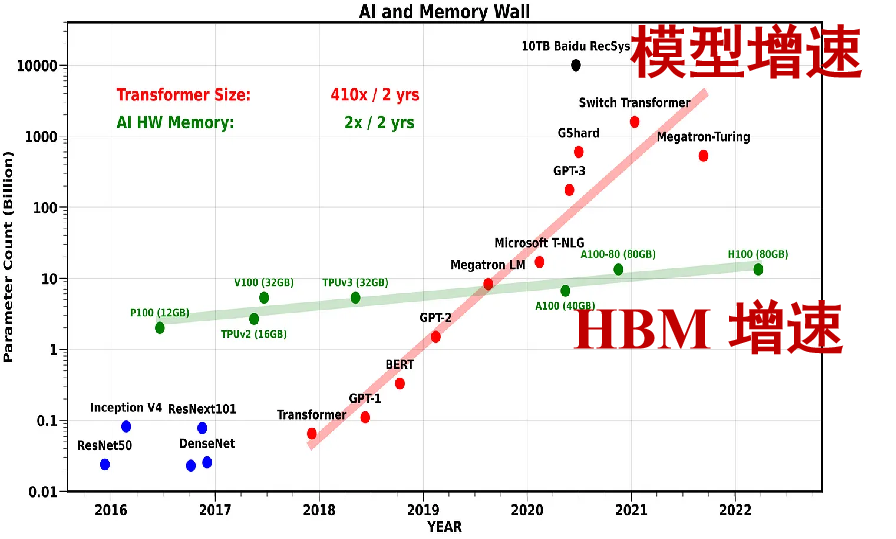
\includegraphics[width=0.8\textwidth]{figure/memory_wall.png}
  \caption{模型参数量增长速度和 HBM 容量增长速度对比}
  \label{fig:memory-wall}
\end{figure}


HBM 作为高带宽访问的存储介质，
是在现代 AI 加速器直接访问的存储资源，在通用高效大模型训练框架中，
需要容纳训练过程中的所有状态，
因此 HBM 容量决定了加速器可训练的模型规模上限。
然而相对于指数级增长的模型规模，HBM 容量增长相对缓慢。
因此单卡 HBM 容量不能够支撑大参数量模型的训练，
主流大模型研发厂商需要用千卡乃至万卡集群进行模型训练。
例如 Meta Llama 3.1 405B 的训练使用了 16384 张 H100 GPU\upcite{meta_llama31_blog}。

相比于预训练，微调虽然总数据量较小，总计算量和训练时间较少，
但是 AI 加速器端仍承受较大的存储压力。全量微调场景下，模型参数、
梯度和优化器状态等都需要完整存储，中间激活也需要保存，
这会占用大量的 HBM 资源。上述情况意味着在资源有限的情况下，
微调受限于在训练过程中存储资源能否容纳训练的状态，
以及状态在训练迭代过程中能否高吞吐地访问和迁移。

本文所关注的企业和研究者等资源受限微调任务需求者
通常难以部署大规模计算集群来完成微调任务，仅能够负担少量节点。
对于这些使用者，需要保证模型能够完成微调，
且微调速度、收敛稳定性处于可接受范围。

与此同时，自主可控的国产计算平台逐渐成为重要的基础设施。
例如华为昇腾面向训练、推理提供了较为完整的软硬件体系，
Atlas 系列服务器被运用于 AI 训练、后训练和推理场景。
MindSpeed 框架支持大模型的预训练和微调流程。
平台形成了围绕 AI 处理器、主机 CPU、CANN 软件包
的全栈生态，能支撑模型的微调。
但与国际先进 AI 加速卡相比，
华为加速卡在 HBM 容量上存在更明显限制，
例如相比于英伟达 Blackwell 架构加速卡达 192GB 的 HBM 容量，
Ascend 910B 的单卡容量仅为 64GB。因此，
在国产计算平台上进行大模型的微调，
HBM 容量的限制更严峻。

硬件资源的限制问题，通过系统软件侧存算调度技术能有效缓解。
通过在计算和存储之间进行权衡和合理的调度能降低训练过程中对 HBM 的需求。
通过在计算与数据迁移之间进行协调，
在不同层级的存储介质之间对模型状态和激活值进行合理的分片与迁移，
就能够在可接受的性能损失下降低对 HBM 容量的依赖。
特别是对于后训练中的微调场景，面对相对有限的数据量和固定的模型结构，
存储扩展和计算通信重合具有较好的收益。

基于以上认识，
本文围绕国产昇腾平台，在资源受限的场景下展开大模型微调存算调度技术的研究。
该研究具有如下意义：

降低大模型微调中异构存储张量迁移的显式开销。
传统的执行模式要求所有模型状态必须驻留在 HBM 中，制约了可微调的模型规模。
本文分析计算强度与传输带宽之间的定量关系，
探索异构存储层级间的张量迁移，
构建异构存储间的流水线重叠方案。
本文方案为分布式系统下的存算解耦提供了参考，
说明在有限 HBM 约束下，通过合理的调度和时序控制，
可以提升模型微调规模
并取得比现有存算调度系统更高的微调性能。

有助于挖掘国产算力平台的功能和性能潜力。
本文基于国产算力平台，参照其性能参数进行系统设计，
基于其生态进行系统实现，在平台上进行专门性能优化和实验验证。
最终实现了大模型微调存算调度系统原型。
研究期间经验和实现的原型有助于后续其他研究者对国产算力平台的进一步探索。

有助于中小企业及科研单位利用国产设备进行模型微调。
当前，人工智能正成为驱动产业升级的引擎，而大模型是该引擎的关键环节。
随着自主可控要求的不断提升，构建基于国产算力底座的大模型微调能力具有现实需求。
然而，国产计算卡的存储资源相对稀缺，同时企业和研究机构也无法得到足够资源。
本文的研究工作探索了降低对高昂硬件资源依赖的方法，
使得在有限的算力节点上开展千亿级参数模型的微调成为可能。
有助于中小企业及科研单位利用国产设备进行特定领域知识学习、安全性对齐以及
行业场景适配。


\section{国内外研究现状}
在资源受限的场景下，存算调度技术涵盖
分布式任务调度和异构设备利用
等多层面方案。

由于模型参数量增长，单张人工智能加速卡所有的存储容量和算力
不能满足大模型微调需求，
因此微调时需要将模型分布在多张加速卡上。
分布式并行策略包括数据并行（DP）、
张量并行（TP）、流水并行（PP），针对长序列的序列并行（CP）和针对混合专家模型的模型并行（EP）。
这些并行策略分别从样本、张量、模型深度、序列和专家网络等维度切分训练负载，
是当前大模型训练系统扩展规模的基础。

数据并行作为基础的并行方式，在每张加速卡上复制一份模型参数，
并将每一批次训练数据分散到不同加速卡上，在每一轮次结束时通过通信原语进行同步，
此并行方式充分利用了算力\upcite{sapio2021switchml}。

在算力资源受限的背景下，针对传统数据并行无法实现存储节省的问题，
微软提出的 ZeRO 技术通过将参数、
梯度和优化器等模型状态进行分片，使其分布在不同的加速卡中，从而消除冗余，
减少HBM占用\upcite{rajbhandari2020zero}。该技术分为ZeRO-1/2/3三种模式，分别分片优化器状态、优化器状态与梯度，
以及整个模型状态，不同程度地节省了单卡HBM。

流水并行、张量并行和专家并行方案沿着参数的不同维度
将模型的切分并分配到不同计算卡上，使得
每张计算卡只需要存储和计算模型的某个部分。
流水并行按深度切分模型，切分后的模型块输出是另一个模型
块输入。该方案需要采用特定调度方式减少流水线气泡
\upcite{huang2019gpipe,harlap2019pipedream}。
张量并行则将单层内的矩阵乘法和不同注意力头切分
到不同设备中。对于稀疏激发的混合专家模型，
专家并行则将不同的专家子网络分布在不同设备上，
根据路由机制将数据动态分发至对应的专家所在的设备进行计算，
从而在不显著增加计算量的同时极大扩展了模型的参数规模。

针对长序列输入带来的存储占用，
序列并行通过在序列维度上对输入数据进行切分，
通常使用环形注意力的实现解决注意力计算的卡间依赖，
将注意力存储占用分散至多卡。
该方法支持了超长上下文训练\upcite{liu2024ringattention}。

在实际的大模型训练中，通常会根据硬件拓扑和模型特性，
采用上述多种方式的混合并行策略以实现效率最大化\upcite{shoeybi2019megatron,narayanan2021megatron}。
图\ref{fig:5d-parallel}概括了多种并行策略在多维并行中各自切分的维度。

\begin{figure}[!htbp]
  \centering
  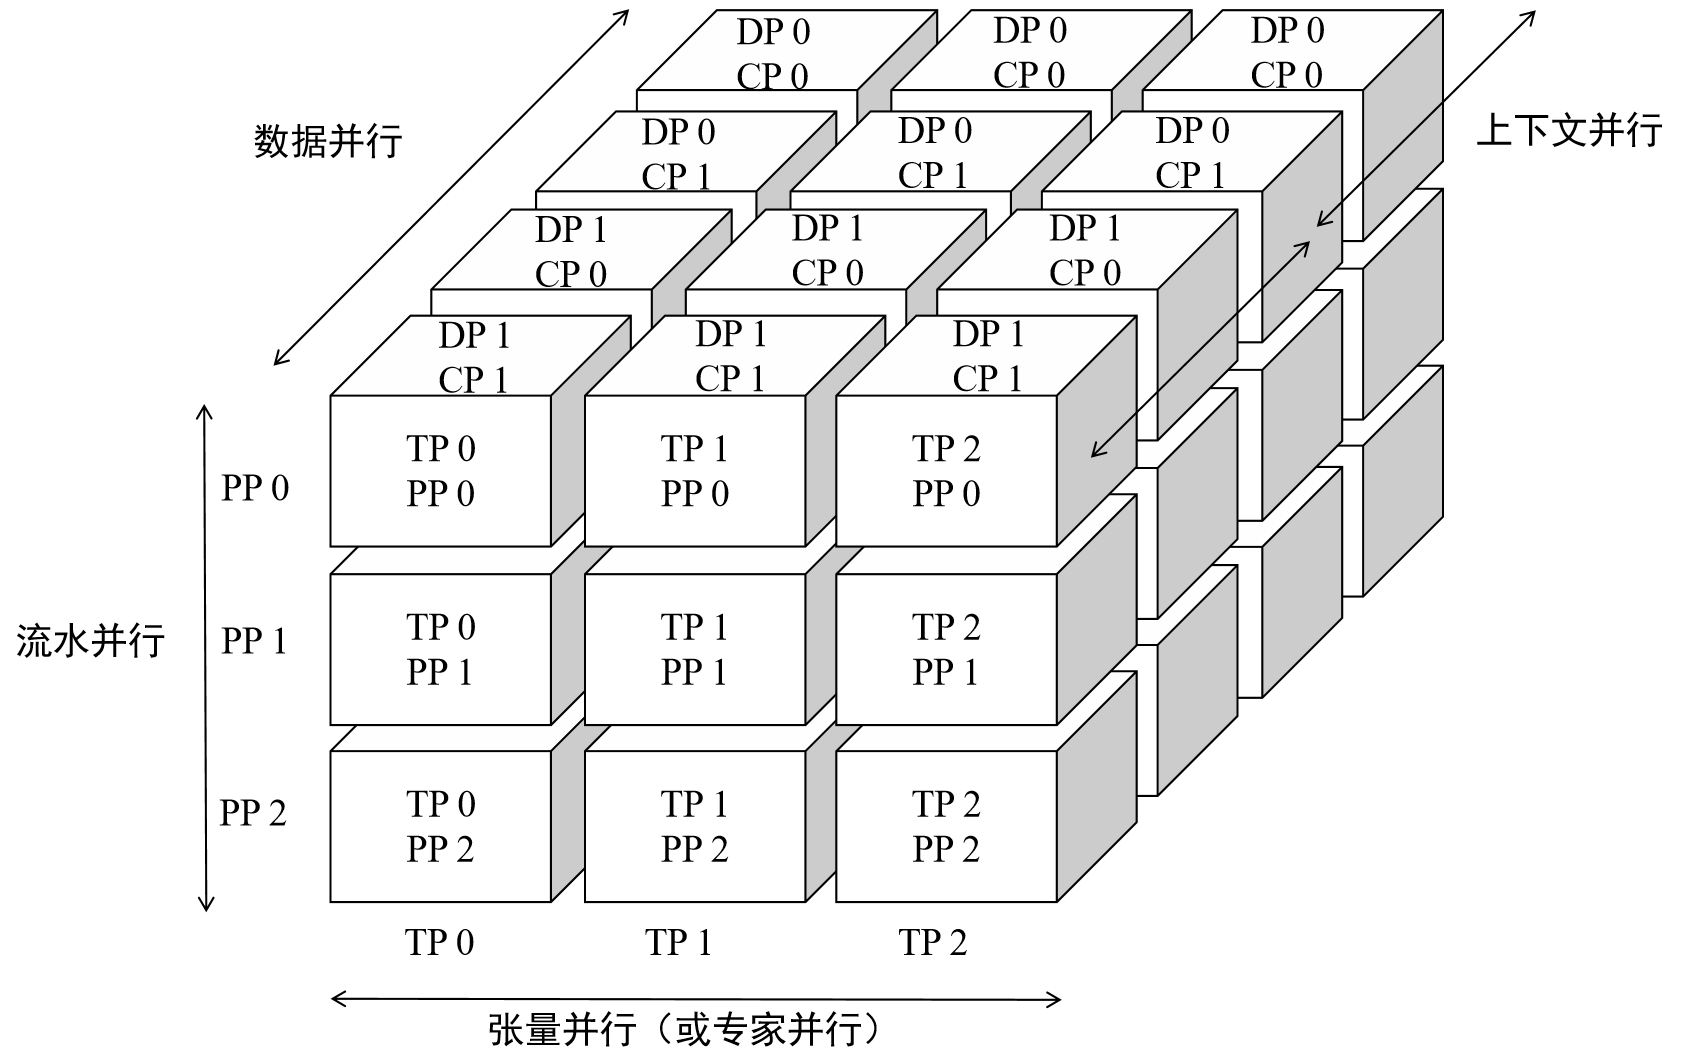
\includegraphics[width=0.85\textwidth]{figure/5D_para.png}
  \caption{五维并行策略示意图}
  \label{fig:5d-parallel}
\end{figure}

但在微调超大模型或HBM极度受限的场景下，即便使用了 ZeRO-3 全分片或使用 TP-PP 组合的并行方式，
单卡存储仍可能不足以容纳分片后的状态。此时就需要在异构设备利用层面进行存算调度，即使用模型卸载技术。
卸载技术针对利用异构存储层级如主机CPU内存、NVMe SSD
等来扩展HBM容量以解决静态的模型状态导致的HBM溢出问题。
ZeRO-Offload 是该领域的代表性工作，其基于ZeRO实现\upcite{ren2021zerooffload}，
将优化器状态以及梯度更新计算常驻主机 CPU 内存中执行。在训练的前向传播和反向传播阶段，
它只将当前层所需的模型参数从 CPU 动态加载至 GPU HBM，计算完成后立即释放或写回，
而梯度则在反向传播过程中被累积并同步传回 CPU。
该技术显著提高了单张加速卡所能训练的模型参数量，使得在有限资源下训练百亿参数模型成为可能。

为了进一步突破 CPU 内存的容量限制，ZeRO-Infinity
引入了 NVMe SSD 作为更底层的存储介质，构建了一个包含 GPU HBM、CPU 
内存和 NVMe SSD 的调度机制\upcite{rajbhandari2021zeroinfinity}。

\section{问题与挑战}
模型卸载技术是解决本研究面对的资源受限场景的大模型微调问题的良好技术路线，
但现有的技术存在两大问题。
其一是扩展性问题，上述卸载技术多基于 DeepSpeed 框架进行开发，
其对张量并行和流水并行等并行方式支持不足，
通常仅支持使用 DP 方式进行扩展\upcite{rasley2020deepspeed}。
因此，这类系统难以充分结合张量并行、流水线并行等分布式任务调度策略。
其二是生态受限问题，一些卸载技术如
LoHan，以及 ZeRO 系列的 Superoffload 是基于 CUDA 生态的原型系统，
其中 Superoffload 还依赖于硬件特性，
在国产环境中难以直接使用\upcite{liao2024lohan,yin2025greedysnake}。

因此，本工作拟基于国产设备特性独立设计与实现新的存算调度机制，
从而达到在可微调的参数量上大于国产平台的原生系统。

尽管模型卸载技术能够扩展存储边界、提升可微调规模，
但在资源受限的国产计算环境下，
要与张量并行、流水线并行等策略共同工作并保持较高吞吐，
仍面临多重挑战。

(TODO 挑战还需润色)
（要搞清楚为什么 zero 比我慢。）

首先是多层存储系统的设计和管理存在挑战。
需要在可微调规模和运行性能之间做出权衡，
既要能够增大可微调的模型参数规模，又要使得
微调执行效率足够。将张量迁移到主存乃至
外存，可以扩展微调规模，但频繁的迁移或不恰当的向外存的迁移
会引入数据传输开销，从而影响微调效率。
因此需要决定微调过程中的各种张量
的生命周期进行建模和追踪，并设计其在不同时间点
的驻留位置。同时还
需要张量的统一管理机制，否则容易引发
张量由不同层级软件栈被重复管理导致内存未能及时释放
、内存碎片或设备迁移时对齐约束不满足等问题。


其次是流水线设计和由引入的
异步流与异构算力间的同步存在挑战。
需要合理设计流水线来实现高效计算数据传输重叠，
而不是需要了再取。
另外预取和流水线下，卸载、加载、计算和缓冲复用存在复杂依赖关系，
使用 NPU 和 CPU 协同计算也有依赖关系。

最后是多维混合并行策略下张量生命周期追踪复杂性增加。
在融合分布式并行策略如结合张量并行、流水线并行时，
模型计算顺序由流水线并行
调度策略决定，同一时刻系统存储中可能需要驻留
多个微批次的激活值，同一模块可能在同一步骤中
重复出现。这需要系统构建统一的张量索引
进行张量定位，根据运行时信息进行张量迁移，以保证系统的正确性。


\section{研究目标和内容}

本工作面向资源受限环境研究大模型微调的存算调度技术，
针对国产昇腾计算平台的存储层次结构与带宽特性，
研究并实现一套兼容分布式并行，
以模型卸载为核心模块的存算调度系统。
系统整体目标是在严格受限的存储条件下，
同时提升可支持的模型规模、
维持较高微调性能，
并保证大规模微调任务稳定完成。

在规模方面，
本工作的核心目标是在单节点环境中
支持参数规模不低于千亿级别的大模型
全量微调任务。
在多节点环境中能实现模型规模的进一步扩展。
在启用梯度累加与全量重计算策略的前提下，
微调过程中峰值存储占用小于
硬件物理上限，不发生任一存储层级的内存溢出错误。

在性能方面，
由于引入主机内存与固态存储作为扩展存储层，
不可避免地带来额外的数据迁移开销。
本工作的目标是通过异步执行流与
细粒度预取机制，
将跨介质数据传输的延迟
最大程度地掩盖在模型计算过程中。
在典型大模型微调配置下，
由数据迁移引入的端到端性能下降
应控制在原生无卸载训练性能的50\%以内。
通过优化数据访问时序与流水线调度策略，
使计算设备在利用率尽可能提高，
避免因数据未及时就绪而导致的执行停顿。

在任务可完成性方面，
本工作需要
保证训练过程的稳定性。
在计算和参数更新过程中
确保数值与原系统的一致性，
微调任务能够顺利完成。

围绕上述目标，
本研究首先建立大模型微调过程中的
 HBM 占用模型。
通过系统分析前向传播、
反向传播以及优化器更新三个阶段中
各类张量的生命周期特征，
对模型参数、梯度、优化器状态
以及中间激活值进行建模，
从而获得训练过程中存储占用
的峰值分布和随时间变化特征。

在此基础上，
设计统一的多级内存管理机制，
以适配加速器 HBM、
主机内存以及外部存储
构成的层次化存储体系。
通过构建统一的张量管理框架，
实现不同存储层之间的协同调度，
并采用预分配内存池与动态复用策略，
减少频繁内存申请与释放带来的额外开销，
同时避免内存碎片问题。
该机制还需保证张量在不同存储层级之间迁移时
满足地址一致性与对齐约束，
从而确保计算图执行的稳定性。

此外，
本研究设计异步卸载与调度引擎，
实现计算与数据传输的高效重叠。
系统根据模型执行顺序与硬件带宽特征，
构建跨层级的数据迁移路径，
对非活跃张量进行提前卸载，
并通过预取机制在计算发生前完成数据加载。
从而提升整体系统吞吐。

最后，
在系统实现层面，
本工作基于 MindSpeed 框架完成上述机制集成，
并在 Atlas 昇腾计算平台上进行实验验证。
通过在不同模型规模与并行配置下的对比实验，
从可微调规模、训练吞吐以及可扩展性等维度
评估系统性能，
验证所提出存算调度机制的有效性与实用性。

\section{本文组织架构}
本文分为五章。

第一章为绪论。介绍本设计的选题背景、研究意义，
分析国内外研究现状后指出本研究的
目标和内容。

第二章为相关技术基础。概述了大语言模型
的基本结构和微调过程中的存储占用情况。
介绍了常用的模型训练的并行方式。结合
存储介质分析了现有的存算调度技术。

第三章为本系统的总体设计。首先根据
硬件参数对设计思路进行了分析，给出了
系统总体设计。其次介绍了各层级存储
的张量组织方式。最后介绍了系统的
通信计算流水线设计。

第四章为本系统的模块和实现介绍。介绍了
本系统的执行引擎和存储管理两大模块
在 MindSpeed 框架中的实现方式。

第五章为实验结果和分析。介绍本系统
在国产软硬件环境中，在资源受限的场景下
微调模型的性能，涵盖单卡、多卡和多机
场景，验证了相对于其他系统可微调规模的
提升、微调端到端吞吐量的提升；同时
分析了各个模块的作用。

\chapter{相关技术基础}
\section{大模型微调的负载和存储占用}

（TODO 我想要得到的结果是
1. transformer 图展示一下，上面写参数
2. 微调和 micro acc 一起介绍完，把所有参数一写
3. 最后才得到 memory 分析结果）

\subsection{大模型微调技术}
大语言模型是人工智能领域智能体的基座。其通常是基于 Transformer 架构
的深度神经网络，由数十到上百同构的 Transformer 层深度堆叠而成。
为便于后续分析，下面定义决定 Transformer 模型规模的几个配置参数。
模型层数为 $L$，隐藏维度为 $H$，
注意力查询头数为 $A_q$，键值头数为 $A_{kv}$,
前馈网络中间层维度为 $D_{\mathrm{ff}}$。

注意力模块中查询、键、值及输出投影均由线性映射构成，
其参数规模可表示为
\[
\Phi_{\mathrm{attn}} =
2H^2 + 2H^2 \cdot \frac{A_{kv}}{A_q}
\]

前馈网络由两层全连接构成，其参数规模为
\[
\Phi_{\mathrm{ffn}} = 2H D_H
\]

因此单层 Transformer 的参数规模为
\[
\Phi_{\mathrm{layer}} =
2H^2 + 2H^2 \cdot \frac{A_{kv}}{A_q} + 2H D_H
\]

进一步，忽略输入输出和 Norm 层，整体模型参数规模可近似估计为
\[
\Phi = L\left(2H^2 + 2H^2 \cdot \frac{A_{kv}}{A_q} + 2H D_H\right)
\]



构建大语言模型时，研究者仅预先定义网络逻辑结构，
而决定实际输出的模型参数需要用数据驱动的方式得到，
即给定数据和损失函数，通过优化算法对模型参数进行迭代，
使模型输出逼近目标分布。
这个基于数据的参数优化过程称为训练。

模型训练包含预训练与后训练两个阶段。
预训练通过模型在大规模无标注数据上进行自监督学习，
使模型获得通用的语言能力；后训练通过改进数据和损失函数计算方法
进一步优化模型参数，以便满足应用需求
通常包括监督微调和人类反馈强化学习等环节。

微调是后训练阶段的重要组成部分。在预训练模型基础上，
其使用特定任务或特定领域的数据进行训练，
从而使得模型的输出分布更符合目标任务要求，
能够学习遵循指令并生成符合人类预期的回复。

微调过程对于模型在专业领域的部署具有重要作用。
通过使用领域相关语料，
微调能够有效注入领域知识，减少幻觉，增强安全性
约束，有助于模型从仅能生成通用语言
转化为能高效解决特定领域的专业任务。

相比于预训练阶段，微调所使用的语料总量较少
，因此训练时所需的总 FLOPS 较少。通常预训练
需要数万亿词元，而微调通常消耗数百万到数亿词元。
但微调和预训练在计算逻辑上一致。
两者均包含前向传播以及反向传播和参数更新三个阶段，在存储资源占用方面也表现出相同的特征。
模型的预训练或微调过程分为三个阶段，分别是前向传播、反向传播和参数更新阶段。
前向传播阶段根据当前参数和输入计算模型生成的输出，并与预期输出计算损失值。
反向传播阶段依据链式法则，根据最终计算出的损失值和前向传播阶段保存的激活值
计算出损失值对每个参数的梯度。参数更新阶段使用优化器，以反向传播得到的梯度
以及历史梯度矩为依据对当前参数进行一轮更新。

在上述计算流程中，梯度计算依赖于前向传播过程中保留的中间激活值，
这些中间激活值在自动微分的实现中无法释放；同时大量模型状态张量
在训练过程中也需要常驻存储。由于微调过程在计算图结构上和预训练
一致，尽管微调迭代次数较少，但单步训练过程中的瞬时存储占用
并不会降低。这意味着微调过程中大量存储资源需要被占用。

为了降低微调对存储资源的需求，研究者提出
参数高效微调的方法。 例如 LoRA 通过原权重上
引入低秩可训练参数 减少了需要训练的参数量，
同时保持较好模型性能\upcite{hu2021lora}。
由于需要计算梯度的参数规模缩小，
参数高效微调方法能够降低 HBM 需求，
提升实验效率。
然而参数高效微调与全量微调在优化轨迹和最终解上不等价，
无法代替全量微调。
一些研究表明 LoRA 可能与全量微调表现出显著差异。
例如标准低秩配置的 LoRA 相比全量微调
在数学推理上准确率下降 5-15 个百分点，
在代码生成任务上下降 3-10个百分点
\upcite{biderman2024loralearnsless}。
因此在追求任务效果的企业和研究者中，
全量微调仍具有不可替代的重要性。

另一方面，即使使用了参数高效微调技术，
在资源受限情况较严重时，仍然不能够进行
大模型的微调。例如，如果当单个 AI 加速卡
不能容纳参数时，无法进行微调。
因此，需要使用存算调度技术，
进一步降低峰值内存占用。


\subsection{大模型微调存储占用模型}

在微调的前向传播、反向传播、参数更新
三个阶段的计算过程中，存储资源的占用分为两部分，一部分为模型状态占用，
该部分为静态占用，需要在整个微调流程中占据固定大小的存储空间。
另一部分为动态占用，在微调流程中周期性增长和消亡。

模型状态包含参数、梯度和优化器状态。为了保证数值稳定性和执行训练高效性，
微调框架普遍采用 BF16 混合精度训练机制。假设模型总参数量为 $\Phi$，
在前向传播和反向传播阶段参与计算的张量为 BF16 格式，
故参与计算的参数与梯度共需占用 $4\Phi$ 字节。

由于存储资源有限，较大训练批次下中间状态难以被容纳，
微调框架常采用梯度累加技术。该技术通过将一个全局批次分成多个微批次进行前向传播和反向传播，
并将梯度累加至独立的缓冲区以完成大批次的训练，待达到预设步数后再进行全局的参数更新。
为了防止在多步累加过程中产生数值舍入误差并损失精度，
系统需要额外存储一份 FP32 精度的梯度用于累加。
同时，以 AdamW 优化器为例，优化器状态需要存储 FP32 格式的主参数、
FP32 一阶动量和 FP32 二阶方差。
这意味着系统共需要提供 $20\Phi$ 字节的静态存储空间。

动态占用的存储空间主要包括激活值状态、通信缓冲区
和碎片开销。其中以激活值状态为核心占用。
在自动微分机制下，在前向传播阶段生成的中间特征张量
需要滞留在存储中，以作为反向求导环节的数据依赖。
假设序列长度为 $S$。

设微批大小为 ${\mu}$，隐藏维度为 $H$，模型层数为 $L$，则单层激活占用可表示为
\[
M_{\mathrm{act}}^{(l)} = S \cdot \mu \cdot H + S \cdot \mu \cdot H + S \cdot \mu \cdot D_H
\]

其中第一项对应注意力输入激活，第二项对应注意力输出激活，第三项对应前馈网络中间激活。

整理可得单层激活规模为
\[
M_{\mathrm{act}}^{(l)} = S \cdot \mu \cdot (2H + D_H)
\]

因此整体模型激活占用为
\[
M_{\mathrm{act}} = L \cdot S \cdot \mu \cdot (2H + D_H)
\]

由此可见，在 $L$ 与 $H$ 固定的情况下，
激活占用与序列长度 $S$ 和微批次大小呈线性关系。
随着序列长度和批大小增加，激活值可能超过静态占用，
成为微调过程中的主要存储开销。

激活值的动态属性体现在只有某层进行了前向传播计算得到激活值
才会占用存储空间，等反向传播到达该层，计算得到梯度以后，
激活值即可释放。因此在微调过程中，存储占用呈每个微批次出现一个峰值的特征。
下面展示了特定配置下 HBM 占用的时间线图。（TODO 有图）

\section{大模型微调的存算调度技术}

在资源受限场景下，存算调度技术优化
资源分配机制以缓解资源瓶颈，通过干预
计算流与数据流，提升存储资源利用率。在
集群配备多张加速卡的场景下，可以将微调
过程的状态平均分布到不同单元上，以缓解
一个单元的存储压力，分布式并行策略即
使用该方案。针对激活值存储占用随序列长度增长
的问题，可以以计算换存储，减少存储占用，
相关技术称为重计算。
当存储资源与模型规模对比更悬殊时候，
需要使用异构存储扩展 HBM，相关技术称为模型卸载。

\subsection{分布式并行策略}

当单卡难以容纳模型完整训练状态时，分布式
并行策略在多节点间分配负载与存储。该技术
降低单卡存储压力，并协同使用多卡算力。
下面介绍与本工作相关的数据并行、张量并行和
流水并行方案。

数据并行在各节点分配训练数据，并复制完整
模型副本以加速训练。该方法充分利用各计算卡的算力，
但未通过增加设备降低单卡存储占用。ZeRO 机制
针对传统数据并行不能降低单卡存储占用的问题，
提出状态分片方案，将参数、梯度与优化器
进行切分以消除冗余。ZeRO-1/2/3 分别对优化器、
优化器与梯度，及完整状态进行分片，逐步
减少存储占用。
（TODO ZERO-1/2/3 图片）

（TODO 张量并行图）

张量并行利用矩阵分块性质将权重划分至多卡，
用以解决单层规模过大难以被单张计算卡容纳的问题。
Megatron-LM 框架定义了
算子分割方案。以 MLP 前向传播为例，MLP 输出满足
$Z = f(XA)B$。针对输入 $X \in \mathbb{R}^{b \times s \times h}$，
升维层 $A$ 采用列切分策略，划分为
$A = [A_1, A_2, \dots, A_N]$，
子矩阵 $A_i \in \mathbb{R}^{h \times h'/N}$ 分布
于单一计算单元。各单元接收全量输入 $X$，
计算局部激活 $Y_i = f(X A_i)$，随后
不需要进行通信，而是将降维层 $B$ 采用行切分策略，
划分为 $B = [B_1; B_2; \dots; B_N]^\top$，
其中 $B_i \in \mathbb{R}^{h'/N \times h}$。
依据矩阵分块乘法性质，各单元计算部分结果
$Z_i = Y_i B_i$。最终通过一次 All-Reduce
集合通信执行累加。根据以下公式可知上述分块计算方法与原始计算等价。 

$$Z = f(XA)B \
 = [f(X A_1), f(X A_2), \dots, f(X A_N)] [B_1; B_2; \dots; B_N]^\top\
 = \sum_{i=1}^{N} Z_i$$

在自注意力机制中，
各注意力头维度相互独立，可将查询与键值矩阵
按头切分至不同设备。各单元独立计算局部得分
$\text{Attn}_i = \text{Softmax}(Q_i K_i^\top) V_i$，
最终直接拼接得到完整输出。序列并行则进一步
沿序列维度对激活值分区，使层归一化等
算子沿序列长度维度分配到不同计算单元上，优化非线性层显存。

流水线并行将连续 Transformer 层划分为 $K$ 个阶段部署于不同设备，
使各单元仅需维护约 $1/K$ 的模型参数，
用于解决模型深度较大，难以少量计算卡容纳的问题\cite{huang2019gpipe} 。
在此基础上，为降低激活值对存储空间的占用，
PipeDream \cite{narayanan2019pipedream} 提出
1F1B 调度策略，该策略通过尽快执行反向传播的原则，
减少了驻留存储的激活值。其执行流分为预热、稳定与
冷却三阶段。在稳定阶段中，设备完成新微批次前向后，
立即执行旧批次反向计算。由于激活值
在反向完成后立即释放，其峰值存储峰值从与微批次个数
成正比将至常数级。
（TODO VPP 和 PP 流水线图）

此策略在
维持流水线气泡率的同时，支持更大微批次训练。

% 此外，针对长上下文场景，上下文并行在序列维度切分输入
% 张量以应对长序列瓶颈。其将注意力层的计算
% 分配到不同的计算单元上，同时依赖 All-to-All 通信
% 解决不同单元在注意力计算的数据依赖，
% 维持全局注意力计算的正确性并扩展序列长度上限。
% 专家并行适配混合专家架构，将不同专家矩阵放置在不同
% 单元，通过门控路由将 token 分发至
% 激活的专家网络对应的设备，实现参数按需加载。
% 在实际大规模训练场景下，多种并行策略联合使用。

在节点内部，由于有高速互联的存在，卡间通信延迟较低，
张量并行或专家并行是主要方式。而节点之间由于
通信延迟较长，通常采用流水并行或数据并行。
本文所实现的系统面相资源受限场景，不采用传统数据并行。
对多卡和多节点场景，在节点内采用张量并行，
在节点间采用 1F1B 流水线并行，以达到较高效率。


\subsection{重计算技术}

重计算针对模型微调过程中激活值进行存储优化。
模型微调过程通常在模型前向计算时
保存计算图中所有中间节点的激活值，
以便在反向传播计算梯度时直接使用。
这使得激活值所占存储空间正比于模型深度。
梯度检查点技术\upcite{chen2016sublinear}
牺牲了部分计算效率来换取存储空间。
其选择模型的某些子层为检查点。
在前向传播阶段，只保存检查点处的激活值，
反向传播时如需用到非检查点的激活值，
先利用前一个检查点重新运行前向计算，
动态生成激活值随后立即释放。

\begin{figure}[!htbp]
  \centering
  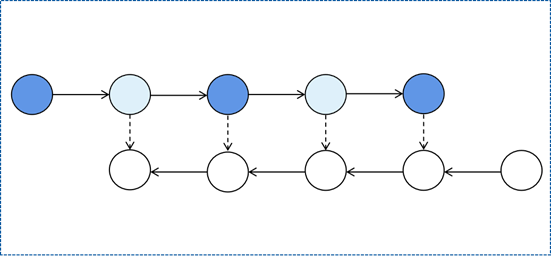
\includegraphics[width=0.8\textwidth]{figure/grad_checkpointing.png}
  \caption{梯度检查点重计算示意图}
  \label{fig:grad-checkpointing}
\end{figure}

如图\ref{fig:grad-checkpointing}所示，
深色计算图结点表示保存相应激活值供反向传播使用，
浅色结点表示激活值在反向传播时重计算。
该技术使模型激活值占用显存
从的空间复杂度从与网络深度成线性正比的 $O(L)$ 
降低到与网络深度平方根成正比的 $O(\sqrt{L})$，
缓解了存储压力。

Flash-attention\upcite{dao2022flashattention} 算子也使用了重计算，
其利用分块方式避免在 HBM 中存储和读取巨大的注意力分数矩阵。
在前向计算时，仅保存必要的统计量用于反向传播，
而将中间生成的注意力矩阵 P 直接释放，
不再回写至 HBM。
在反向传播时，利用前向阶段保存的统计量
以及输入的 QKV 矩阵，重新计算该块内的注意力矩阵 P，
并在 SRAM 中完成梯度的计算与累加，
降低了 HBM 占用并提升了计算效率。

重计算技术与本系统的主要内容是正交的，本系统
的默认实现中也采用全量重计算。
在资源受限程度严重的条件下，
HBM 等存储介质无法容纳模型参数本身、
优化器状态以及必要的梯度缓冲区，
仅依靠重计算技术无法解决存储空间不足的问题。
此时，则需要进一步引入其他显存优化策略，
即针对模型状态进行卸载的技术。


\subsection{异构存储与卸载技术}
大规模模型训练系统建立在由通用处理器、专用加速器与多级存储介质构成的异构体系结构之上。
其中，不同层级存储介质在容量、带宽与访问延迟方面呈现出显著差异，
并共同决定了训练过程中的数据供给能力与系统吞吐上界。

在设备侧，当前主流 AI 加速器普遍集成高带宽存储器(HBM)。
HBM 通过三维堆叠与宽总线设计显著提升数据访问带宽，
其带宽通常达到 TB/s 量级，能够满足大规模张量计算对高吞吐数据访问的需求。
然而，HBM 受限于封装工艺与功耗约束，
其容量通常仅为数十 GB 至百 GB 级别，
难以容纳当前大规模模型训练所需的全部参数、梯度及优化器状态。

在主机侧，动态随机存取存储器 DRAM 构成了第二级存储层。
与 HBM 相比，DRAM 在容量上具有数量级优势，可扩展至 TB 级别，
但其带宽通常低于 HBM 一个数量级，
且需通过 PCIe 等互连总线与加速器通信，
从而引入额外的访问延迟与带宽瓶颈。
因此，DRAM 在训练系统中通常作为容量扩展层，
用于缓解设备侧显存不足的问题。

进一步地，非易失性存储设备 NVMe SSD 提供了更高容量与更低成本的存储资源。
NVMe SSD 的容量可扩展至数十 TB 甚至更高，
但其带宽通常仅为数 GB/s 至数十 GB/s，
且访问延迟显著高于 DRAM。
此外，其访问依赖操作系统 I/O 栈，涉及内核态与用户态切换，
进一步增加了访问开销。
因此，该层通常作为最底层的容量支撑，
用于存放冷数据或进行深度卸载。

基于上述分层存储结构，研究者向大规模模型训练系统集成了多级卸载机制，
以突破单一设备显存容量的限制。
该技术将模型训练过程中不同生命周期的数据对象
包括模型参数、梯度与优化器状态按需迁移至低层级存储介质，
并通过调度策略尽可能掩盖数据传输开销。

（TODO 详细的相关工作介绍，图片展示卸载技术）

针对 HBM 容量不足的问题，
ZeRO-Offload 将部分模型状态从 HBM 卸载到 DRAM。
其放置策略是将模型状态中的优化器状态和梯度卸载到主机 DRAM 内，
并将优化器计算迁移至 CPU 侧执行，而参数和激活值等部分则常驻在
HBM 中。AI 加速器仍承担前向传播和反向传播计算，
在反向传播阶段，梯度一经产生即通过 PCIe 异步传输至主机侧。
为了扩展到多卡场景，ZeRO-Offload 
结合了 ZeRO-2 分片策略，支持用 ZeRO 并行方式进行扩展。
此设计相未卸载情形，显著降低了 HBM 的占用，
CPU 优化器的设计能有效利用 CPU 侧算力，
防止优化器状态反复迁移导致性能下降，同时避免
复杂度与数据大小成正比的前向传播、反向传播计算迁移到 CPU，
保证了微调效率。

% 然而，单纯依赖 DRAM 进行卸载仍难以支撑超大规模模型训练，
% 其瓶颈主要来源于 PCIe 带宽限制及数据传输与计算之间的同步开销。
% 针对这一问题，近期研究工作开始关注计算与数据传输的细粒度重叠。
% 例如，DeepSpeed 后续优化工作通过多流并发与异步拷贝机制，
% 将参数传输、梯度回传与计算过程解耦，
% 并结合基于执行图的预取调度策略，
% 在一定程度上缓解由数据迁移引入的计算停顿问题。

然而，当模型规模进一步扩大时，仅依赖 DRAM 仍无法满足容量需求，
因而需要引入 NVMe SSD 作为更深层的卸载目标。
ZeRO-Infinity 提出构建覆盖 HBM、DRAM 与 NVMe 的多级存储体系，
允许包括参数、梯度、优化器状态在内的张量迁移到 DRAM 和 NVMe SSD。
HBM 仅保存当前算子将要参与计算的活跃张量，以及所需要的参数分片，
其余的参数、梯度和优化器状态则按照用户的不同配置常驻 DRAM 或 NVMe 中。
为了使张量迁移稳定且高效，缓解低带宽的存储设备对性能的影响，
ZeRO-Infinity 使用卸载引擎统一管理不同存储介质之间的数据迁移，
在 NVMe 配置下，其以 DRAM 作为缓冲层，
使张量在 NVMe 与设备之间进行转移，
在 DRAM 中基于锁页内存创建缓冲，缓冲可以进行复用，
CPU 和 GPU 之间、NVMe SSD 和 DRAM 之间的读写可以采用异步 I/O 的形式，
硬盘访问无需同步阻塞。
在某层计算尚未结束时，引擎会为后续层发起预取，
距离较远的数据从 NVMe 读入 DRAM，距离较近的层
从 DRAM 拷贝到 HBM。
在多卡扩展上，其基于 ZeRO-3 将模型状态分片。
当某层需要被预取时候，每张 GPU 只需要保存一部分状态分片，
再通过 All-Gather 通信拼接得到完整参数，该设计既能够
聚合不同 HBM 与主机 DRAM 间的 PICe 带宽。
该工作
将 NVMe SSD 引入模型训练流程，扩展了模型容量边界。
然而这一设计也带来了新的约束，
如果大量张量迁移到 NVMe 中，
模型微调的性能会受 NVMe 带宽的限制，
即使采用流水线限制，其 I/O 开销由于过大，仍无法被隐藏。
因此在微调场景下，选择哪些状态驻留主机 DRAM，哪些状态
进入 NVMe，仍是待解决的问题。

在此基础上，LoHan 指出 ZeRO-infinity 在反向传播重计算存在 
PCIe 空闲、优化器阶段存在 GPU 空闲，卸载流水线仍存在不足。
其在模型状态的基础上进一步卸载激活值，同时对计算-数据迁移流水线进行优化。
LoHan 提出对梯度进行主机卸载，
在主机侧接收到梯度后立即触发 CPU 优化器更新，
从而与设备侧反向传播过程形成重叠。
在激活管理方面，LoHan 观察到 PCIe 资源存在空闲时间，
因此可以进行部分重计算，层内的部分激活进行卸载。
为了确认激活保留量，LoHan 基于模型结构分析，
将迭代时间建模为激活交换量的函数，
并通过搜索确定最优交换策略，
在 HBM 约束与计算开销之间取得平衡。
进行调度流水线优化后 LoHan 相比 ZERO-Infinity
提升了微调性能。
然而 LoHan 系统在多卡扩展上
仅支持简单数据并行，因此不能通过增加加速卡数量提高
可微调模型上限。

（TODO superoffload 要再讲，然后好像有的要配配图）
SuperOffload 系统基于 GH200 硬件，利用 CPU 和 GPU
之间的高速互联，打破了 PCIe 带宽是数据迁移瓶颈的假设。
由于有高速互联的存在，其更积极地使用 CPU 内存和 CPU 计算，
用更细粒度的同划分和参数、梯度、优化器重叠，提高了卸载的效率。
其达到了很高的效率，但是依赖于 NVIDIA GH200/NVLink-C2C 硬件
和 CUDA 生态，也启发我们系统设计需要面向硬件特性。

% 重复了

% 模型卸载技术是解决本研究面对的资源受限场景的大模型微调问题的良好技术路线，
% 但现有的技术存在两大问题。其一是扩展性问题，
% 这些卸载技术多基于 Deepspeed 等框架进行开发，其对张量并行乃至流水并行等
% 并行方式支持不足，进一步扩展的方式受限。
% 其二是生态受限问题，一些卸载技术如由研究者自行实现，
% 它们是基于 CUDA 生态的原型系统，在国产环境中均难以直接使用。
% 因此，本工作拟基于国产设备特性独立设计与实现存算调度机制。

\chapter{系统设计}



\section{存算调度系统的设计分析}

本文面向规模和性能在华为昇腾平台上
设计存算调度机制实现资源受限场景的大
模型微调。设计的目标为单节点上能启动千亿参数量的微调，
支持张量并行和流水并行等方式进行多卡扩展
同时保证性能下降在可接受范围内，
微调可收敛。为了满足这些目标，
系统选择基于 Megatron-MindSpeed 框架设计存算调度方案，使用主机内存
和固态存储作为 HBM 的扩展，在微调过程中对各类张量进行卸载和加载。

\subsection{容量约束与卸载对象分析}

本节分析系统面向规模所需的设计。

百 B 级模型微调中的参数和梯度无法被 HBM 容纳。
设模型参数量为 $\Phi$。
仅 BF16 参数就需要 $2\Phi$ 字节，
反向传播产生的 BF16 梯度也需要 $2\Phi$ 字节。
因此，参数和梯度两项合计为：
\[
M_{\mathrm{param+grad}} = 4\Phi .
\]
对于 130B 参数模型，
该项约为 $520$ GB。
该规模已超过单节点 HBM 总容量，
更不可能全部常驻单卡 HBM。
因此，为了达到大规模的微调，
参数和梯度必须在计算过程中从 HBM 卸载到主机侧。

激活值同样不能全部保留在 HBM 中。
在全重计算的配置下，激活值仅保存
Transformer 层间的激活。
设模型层数为 $L$，序列长度为 $S$，
微批次大小为 $b$，隐藏维度为 $H$。
若每层保存输入和输出两个 BF16 隐藏状态，
则层间激活占用为：
\[
M_{\mathrm{act}} \approx 2LSbH .
\]
以 GLM-130B 为例，
其层数 $L=70$，隐藏维度 $H=12288$。
当序列长度 $S=4096$、微批次 $b=13$ 时，
仅层间激活就需要约 $91.6$ GB。
该数值已经超过单卡 $64$ GB HBM 容量。
因此，激活值也需要从 HBM 卸载到主机侧。

在全量微调场景，BF16 混合精度和 AdamW 优化器配置下，
每个参数除 BF16 计算参数外，还需要保存 BF16 梯度、FP32 主梯度、
FP32 主参数、一阶动量和二阶动量。
如第二章所述，仅模型状态的静态存储需求就约为 $20\Phi$ 字节。
对于 100B 以上参数量的模型，该部分理论占用已经超过 2\,TB。
本文实验平台单节点主机 DRAM 容量为 2\,TB，
实际可用空间还需扣除操作系统、训练框架运行时、张量元数据、
地址对齐和碎片化等开销。
因此，仅使用 HBM 和主机 DRAM
仍无法容纳千亿级模型全量微调所需的全部训练状态。

上述容量约束表明，本文系统不能只采用 HBM-DRAM 两级存储结构，
需要引入 NVMe SSD 作为更深层的容量扩展。
在全部模型状态中，优化器状态占用最大，
包括 FP32 主参数、一阶动量和二阶动量，
合计约为 $12\Phi$ 字节。
因此，从可微调规模角度看，
系统必须将部分训练状态进一步下沉到 NVMe SSD。
基于这一判断，本文采用 HBM-DRAM-NVMe SSD 三级存储结构，
以突破单节点 DRAM 容量对可微调模型规模的限制。

\subsection{计算与通信重叠条件分析}

本节分析系统面向性能所需的设计。

为了使得总体性能下降在可接受范围，
不是所有模型状态都适合卸载到 NVMe。
在微调计算的前向传播、反向传播、参数更新三个阶段中，
前向和反向传播按层访问并产生梯度，其数据迁移效率
影响到 AI 加速器是否能持续进行计算，
而参数更新阶段发生在前向和反向传播结束以后，可以通过梯度
累加降低时间占比。
因此，本节分析前后向阶段数据传播时间被计算时间掩盖的条件，
从而说明参数和梯度等状态适合仅卸载到主机 DRAM。

通过在 Ascend 910B 上对矩阵乘和FlashAttention
算子进行性能测试，可以估计微调过程中单层的计算时间\upcite{dao2022flashattention}。
再结合 PCIe 带宽和 NVMe IO 带宽，可对计算时间
和数据传输时间的时长进行对比分析，从而得到
传输被计算掩盖的条件。

以前向传播为例子。
假设单层模型参数量为 $N$，参数总数据量为：
\[
D = 2N
\]
另假设 HBM 和 CPU 主机内存之间 PCIe 单向带宽为 $B_p$，NVMe IO 单向带宽为 $B_n$，单层平均计算速度为 $P$。则单层 PCIe 传输时间为：
\[
T_{\mathrm{pcie}} = \frac{D}{B_p} = \frac{2N}{B_p}
\]
单层 NVMe 传输时间为：
\[
T_{\mathrm{nvme}} = \frac{D}{B_n} = \frac{2N}{B_n}
\]
对于稠密模型，矩阵乘法和注意力两个模块占据单层前向计算量的绝大部分，因此
用可用矩阵乘法和 FlashAttention 算子的计算量估计单层总计算量：
\[
F_{\mathrm{layer}}(S,b) \approx 24bSH^2 + 4bS^2H
\]
本文使用与目标模型同规模的矩阵乘和 FlashAttention kernel 进行测试，
并只记录这两类主要算子的实测执行时间。
设矩阵乘部分的计算量为 $F_{\mathrm{matmul}}$，
FlashAttention 部分的计算量为 $F_{\mathrm{fa}}$，
两类 kernel 的实测运行时间分别为
$T_{\mathrm{matmul}}$ 和 $T_{\mathrm{fa}}$。
则单层前向平均计算速度估计为：
\[
P =
\frac{F_{\mathrm{matmul}} + F_{\mathrm{fa}}}
{T_{\mathrm{matmul}} + T_{\mathrm{fa}}}
\approx
\frac{24bSH^2 + 4bS^2H}
{T_{\mathrm{matmul}} + T_{\mathrm{fa}}}
\]
其中 $S$ 为序列长度，$b$ 为微批大小，$H$ 为隐藏维度。则单层前向计算时间为：
\[
T_{\mathrm{comp}}(S,b) = \frac{F_{\mathrm{layer}}(S,b)}{P}
\]
若要求计算能够掩盖 PCIe 传输，则需要满足：
\[
T_{\mathrm{comp}}(S,b) \ge T_{\mathrm{pcie}}
\]
代入上式可得：
\[
\frac{24bSH^2 + 4bS^2H}{P} \ge \frac{2N}{B_p}
\]
整理后得到前向计算下满足掩盖条件的微批次 $b$ 的条件：
\[
b \ge \frac{2NP}{B_p(24SH^2 + 4S^2H)}
\]
同理，若要求计算能够掩盖 NVMe I/O，则需要满足：
\[
T_{\mathrm{comp}}(S,b) \ge T_{\mathrm{nvme}}
\]
代入后可得：
\[
b \ge \frac{2NP}{B_n(24SH^2 + 4S^2H)}
\]

因此，在固定模型结构下，掩盖条件由微批次大小 $b$、
单层参数量 $N$、序列长度 $S$、平均计算速度 $P$ 和传输带宽共同决定。
如果其他条件固定，微批次大小增大时，掩盖更容易成立；
参数量增大时，单层传输数据量按 $2N$ 增长，掩盖更难成立；
而带宽增大时，传输时间减小，掩盖所需微批次大小下降。

对于本文使用的华为 Atlas 800T A2 机器，如果使用 GLM-130B 模型，
固定序列长度为 $S=4096$ ，
由上述 kernel 实测方法可得单卡计算单层 Transformer 
前向平均速度为 $197.06$ TFLOPS。
主机 DRAM 和 HBM 间 PCIe 单层有效带宽为 $32$ GB/s，
NVMe 单盘带宽为 $4$ GB/s。
将这些数据带入上述公式可得：如仅使用 DRAM 和 PCIe 间的数据传输，
微批次 $b$ 需要达到 2 以上即可实现计算和传输的掩盖；
而如果使用 NVMe 单盘，则微批次需要达到 13 以上。
图\ref{fig:time-compare}展示了模型单层估计前向计算时间和
DRAM、NVMe 两类数据传输时间的对比。

\begin{figure}[!htbp]
  \centering
  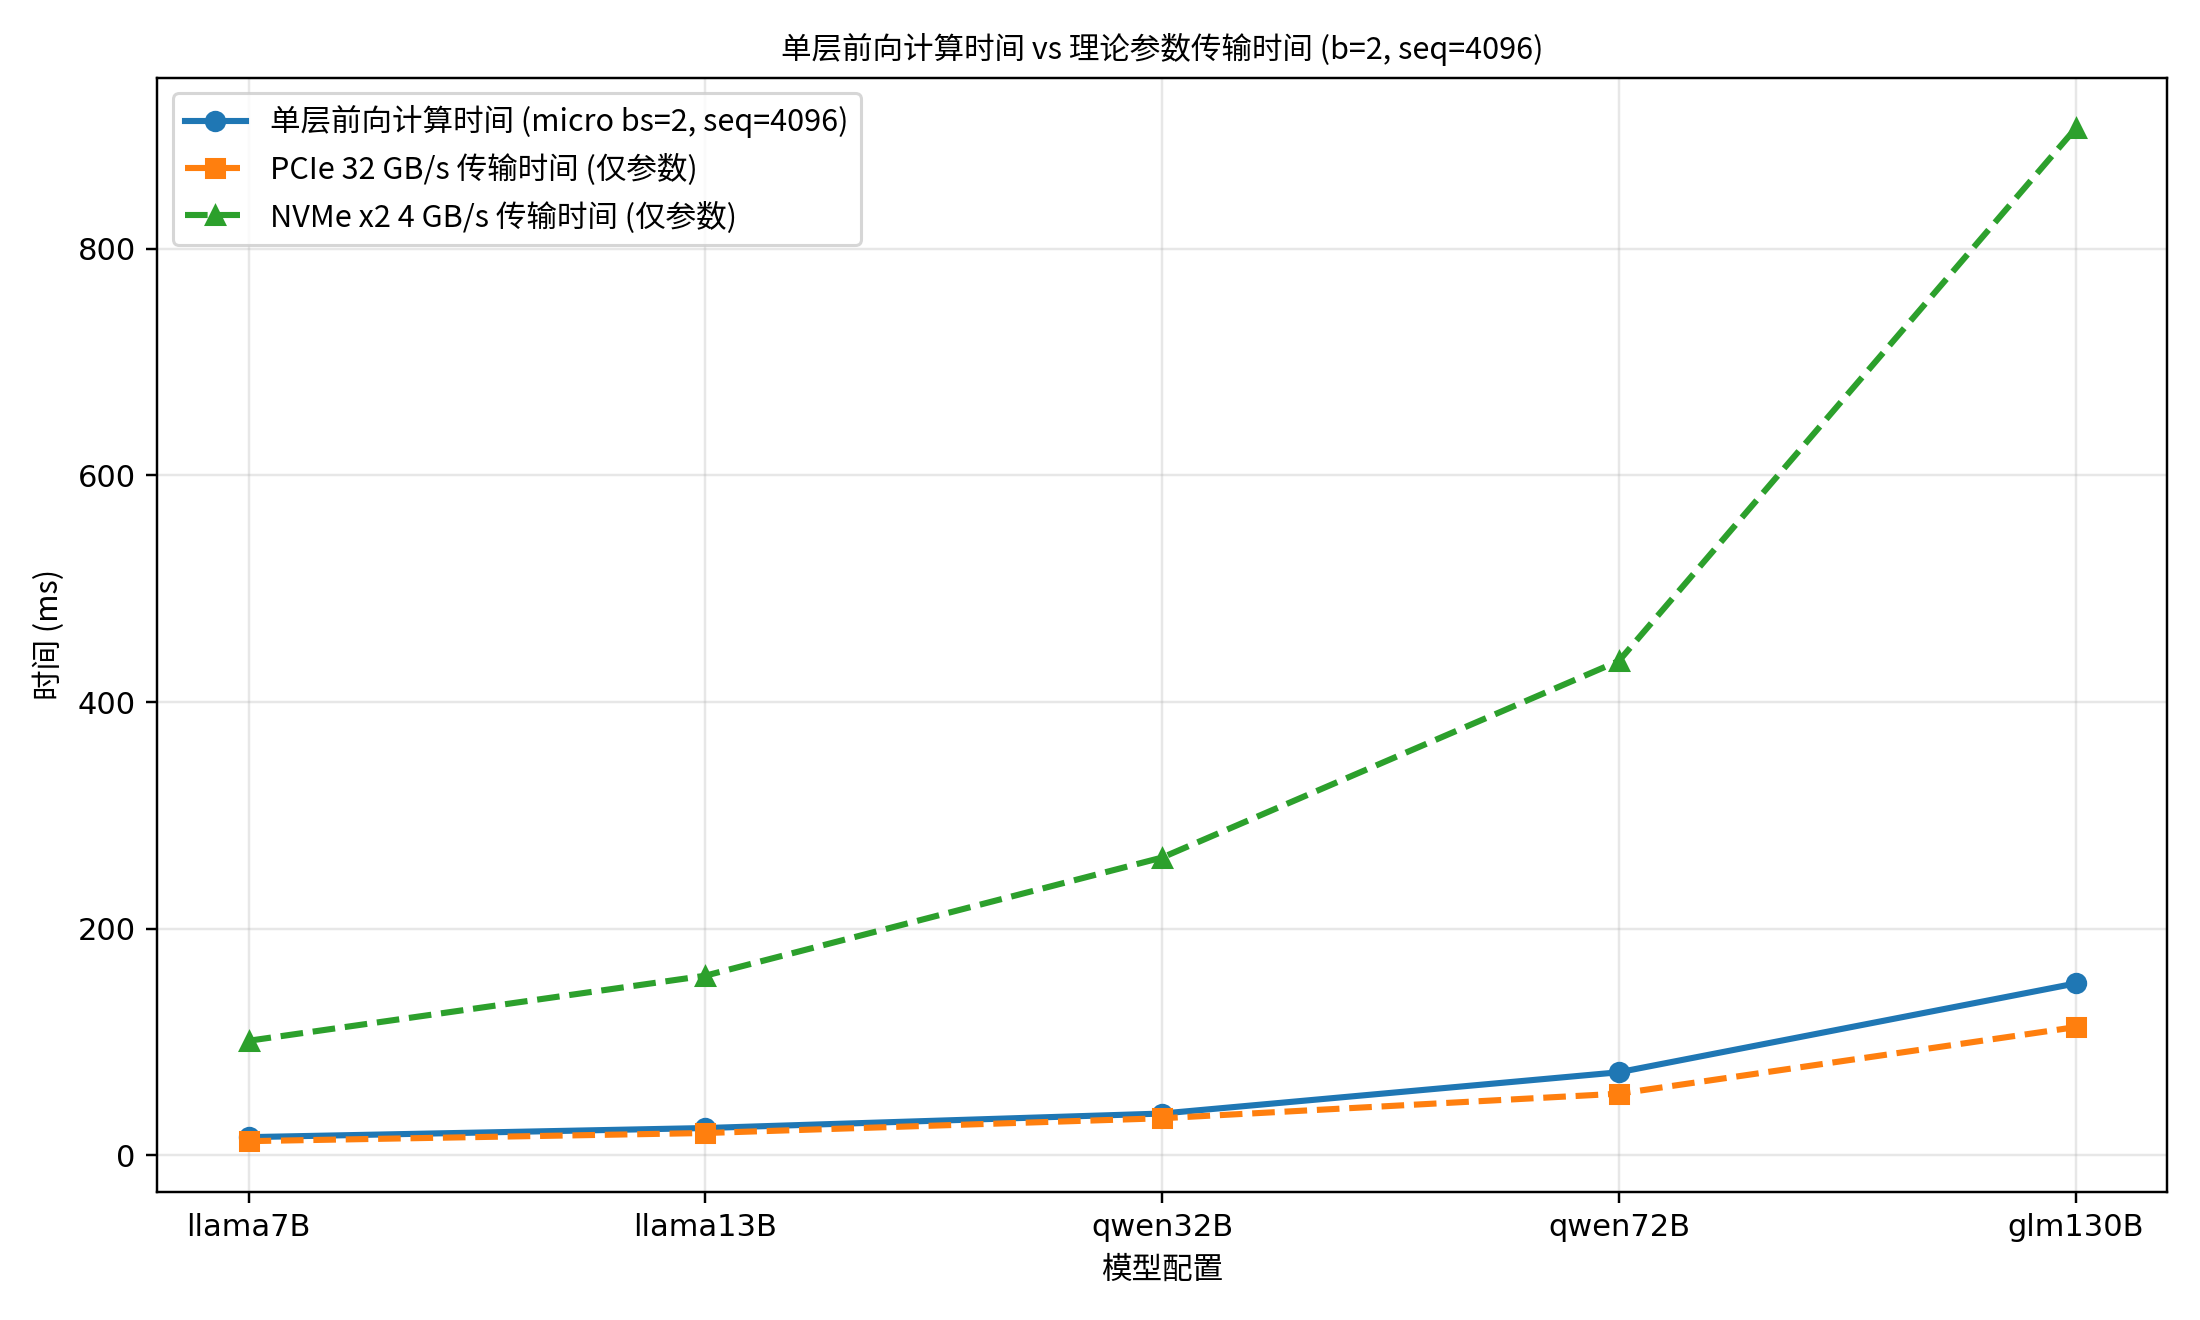
\includegraphics[width=0.8\textwidth]{figure/theoretical.png}
  \caption{估计单层前向计算时间和数据传输时间对比}
  \label{fig:time-compare}
\end{figure}

% $b=13$ 会显著提高单层计算过程中的 HBM 峰值。
% 以 GLM-130B 为例，其隐藏维度 $H=12288$，
% 前馈中间维度 $I=32768$，层数为 $L=70$。
% 首先估计单层前向过程中可能同时活跃的 BF16 激活，
% 包括输入/输出隐藏状态、QKV、注意力输出和前馈中间结果，
% 其峰值可近似表示为：
% \begin{equation}
% M_{\mathrm{act,peak}}^{(l)}
% \approx 2bS(6H+2I)
% \end{equation}
% 代入 $b=13$、$S=4096$ 后，
% 单层激活峰值约为 $14.8$ GB。
% 反向传播阶段还会产生对应的激活梯度，
% 因此单层计算过程中激活相关张量可按
% $2M_{\mathrm{act,peak}}^{(l)}$ 估计。

% 除激活外，单层执行还需要保留参数槽位和梯度缓冲。
% 设单层参数量近似为 $N_l=\Phi/L$。
% 本文的流水线调度至少需要当前计算层参数、
% 下一层预取参数和上一层待卸载参数三个 BF16 槽位，
% 其占用约为 $3\cdot 2N_l$。
% 反向传播产生的 BF16 梯度及其通信/回收缓冲
% 按两份单层参数大小估计，约为 $2\cdot 2N_l$。
% 因此，单层计算过程中的 HBM 峰值可估计为：
% \begin{equation}
% M_{\mathrm{hbm}}^{(l)}
% \approx
% 2M_{\mathrm{act,peak}}^{(l)}
% + 5\cdot 2N_l
% + M_{\mathrm{op}}^{(l)}
% \end{equation}
% 其中 $M_{\mathrm{op}}^{(l)}$ 表示单层算子执行过程中的工作区。
% 本文只估计有明确张量形状来源的算子工作区，
% 不计入通信缓冲和框架运行时预留空间。
% 对于 GLM-130B 的前馈网络，
% gate/up 两个升维投影可视为输出维度为 $2I$ 的矩阵乘。
% 若按 BF16 矩阵乘的 FP32 累加工作区估计，
% 其占用为 $4bS\cdot 2I$。
% SwiGLU 非线性计算还需要一个 $bS\times I$ 的中间工作区，
% 占用为 $2bSI$。
% 因此：
% \begin{equation}
% M_{\mathrm{op}}^{(l)}
% \approx 4bS\cdot 2I + 2bSI
% \end{equation}
% 代入 $b=13$、$S=4096$、$I=32768$，
% 可得 $M_{\mathrm{op}}^{(l)}\approx 17.4$ GB。
% 对于 GLM-130B，$N_l\approx 130\mathrm{B}/70$，
% 则参数槽位和梯度缓冲合计约为 $18.6$ GB。
% 再加上激活及激活梯度约 $29.6$ GB，
% 以及算子工作区约 $17.4$ GB，
% 则单层计算峰值约为 $65.6$ GB，

对于反向传播阶段，单层数据迁移包括参数加载和梯度卸载。
若二者均采用 BF16 表示，
则迁移量约为 $2N+2N=4N$，
是前向参数加载量的两倍。
反向传播需要同时计算输入梯度和参数梯度，
其计算时间通常可近似为前向传播的两倍。
启用重计算后，反向阶段还会重新执行部分前向算子，
可将额外开销近似看作一次前向计算。
因此，反向阶段可用于重叠的计算窗口约为
\[
T_{\mathrm{bwd+recomp}}
\approx 2T_{\mathrm{fwd}} + T_{\mathrm{fwd}}
= 3T_{\mathrm{fwd}} .
\]
即反向阶段传输量约为前向的两倍，
而计算窗口约为前向的三倍。
因此，在 DRAM 路径下，
当前向参数加载能够被计算掩盖时，
反向阶段的参数加载和梯度卸载也通常能够被掩盖。

上述结果说明，若卸载目标为主机 DRAM，
参数预取具有较好的重叠空间。
当微批次达到较小取值时，
单层计算时间即可覆盖 HBM 与主机 DRAM 之间的参数传输。
而 NVMe 路径需要显著更大的微批次才能满足同一条件，
不适合作为前后向逐层高频访问张量的直接来源。

综上，本系统在前后向计算期间避免参数和梯度访问 NVMe SSD，
而将其迁移限制在 HBM 与主机内存之间。
由于单节点主机内存为2T，
能够容纳本文目标规模下的 BF16 参数和 FP32 梯度，
因此这一放置方式同时满足容量和性能需求。

\subsection{张量生命周期与调度分析}

基于上述容量约束与传输重叠条件，
本节根据不同张量在训练迭代中的生命周期设置张量迁移时机。
在微调过程中，参数、梯度、激活和优化器状态的
产生位置、访问阶段和失效时机各不相同，
需要按照各类张量的生命周期设置不同的调度触发点。

参数的生命周期与模块计算边界直接相关。
在前向传播和反向传播中，
每个 Transformer 模块开始计算前都需要读取对应的 BF16 参数。
因此，参数迁移的触发点位于模块计算之前，
系统需要在当前模块执行期间提前为后续模块预取参数。
当某一模块的参数在后续执行顺序中不再被访问时，
其设备侧副本即可释放或被其他模块参数覆盖。

梯度的生命周期始于反向传播阶段。
某层梯度产生后，其在设备侧的主要用途已经结束，
后续主要参与主机侧梯度累加和参数更新。
因此，梯度不需要在 HBM 中长期驻留，
其调度触发点位于模块反向计算完成之后。
系统可以在梯度产生后立即将其卸载到主机侧，
从而减少反向传播过程中设备侧梯度缓冲的峰值占用。

激活的生命周期跨越前向传播和反向传播两个阶段。
层间激活在前向传播中产生，
但要到对应反向传播或重计算阶段才会再次被使用。
其调度过程需要划分为三个阶段：
前向计算完成后写出到主机侧，
反向计算或重计算开始前恢复到设备侧，
使用完成后释放对应缓存。

优化器状态的生命周期与前后向传播相分离。
FP32 主参数、一阶动量和二阶动量
不参与逐层前向传播和反向传播，
只在梯度累加完成后的参数更新阶段被访问。
因此，优化器状态的调度触发点不在模块计算边界，
而在优化器更新阶段。
系统可以在更新阶段按块读入所需状态，
完成 CPU 侧参数更新后再将其写回低层存储，
从而避免优化器状态在前后向阶段占用高层存储空间。


\section{多级存储架构总体设计}
根据前述容量约束、计算传输重叠和张量生命周期分析，
本系统构建了涵盖 HBM、本地内存与 NVMe SSD 的三级存储调度架构。
其中，
HBM 仅保存当前计算阶段参与执行算子的活跃张量，
包括当前模块参数、预取模块参数、反向阶段产生的临时梯度、
重计算所需激活以及算子临时张量；
主机 DRAM 缓存 BF16 参数、FP32 主梯度以及层间激活，
并提供 BF16 临时梯度缓冲和优化器状态工作区；
NVMe SSD 则保存容量较大的优化器状态，包括 FP32 类型的主参数、动量和方差。
该设计既能够保证 HBM 和主机 DRAM 容纳的数据总量可控，
又可以使前向和反向传播中不依赖低带宽 NVMe SSD。
三级存储层次与状态分布关系如图\ref{fig:sys-overall-design}所示。

\begin{figure}[!htbp]
  \centering
  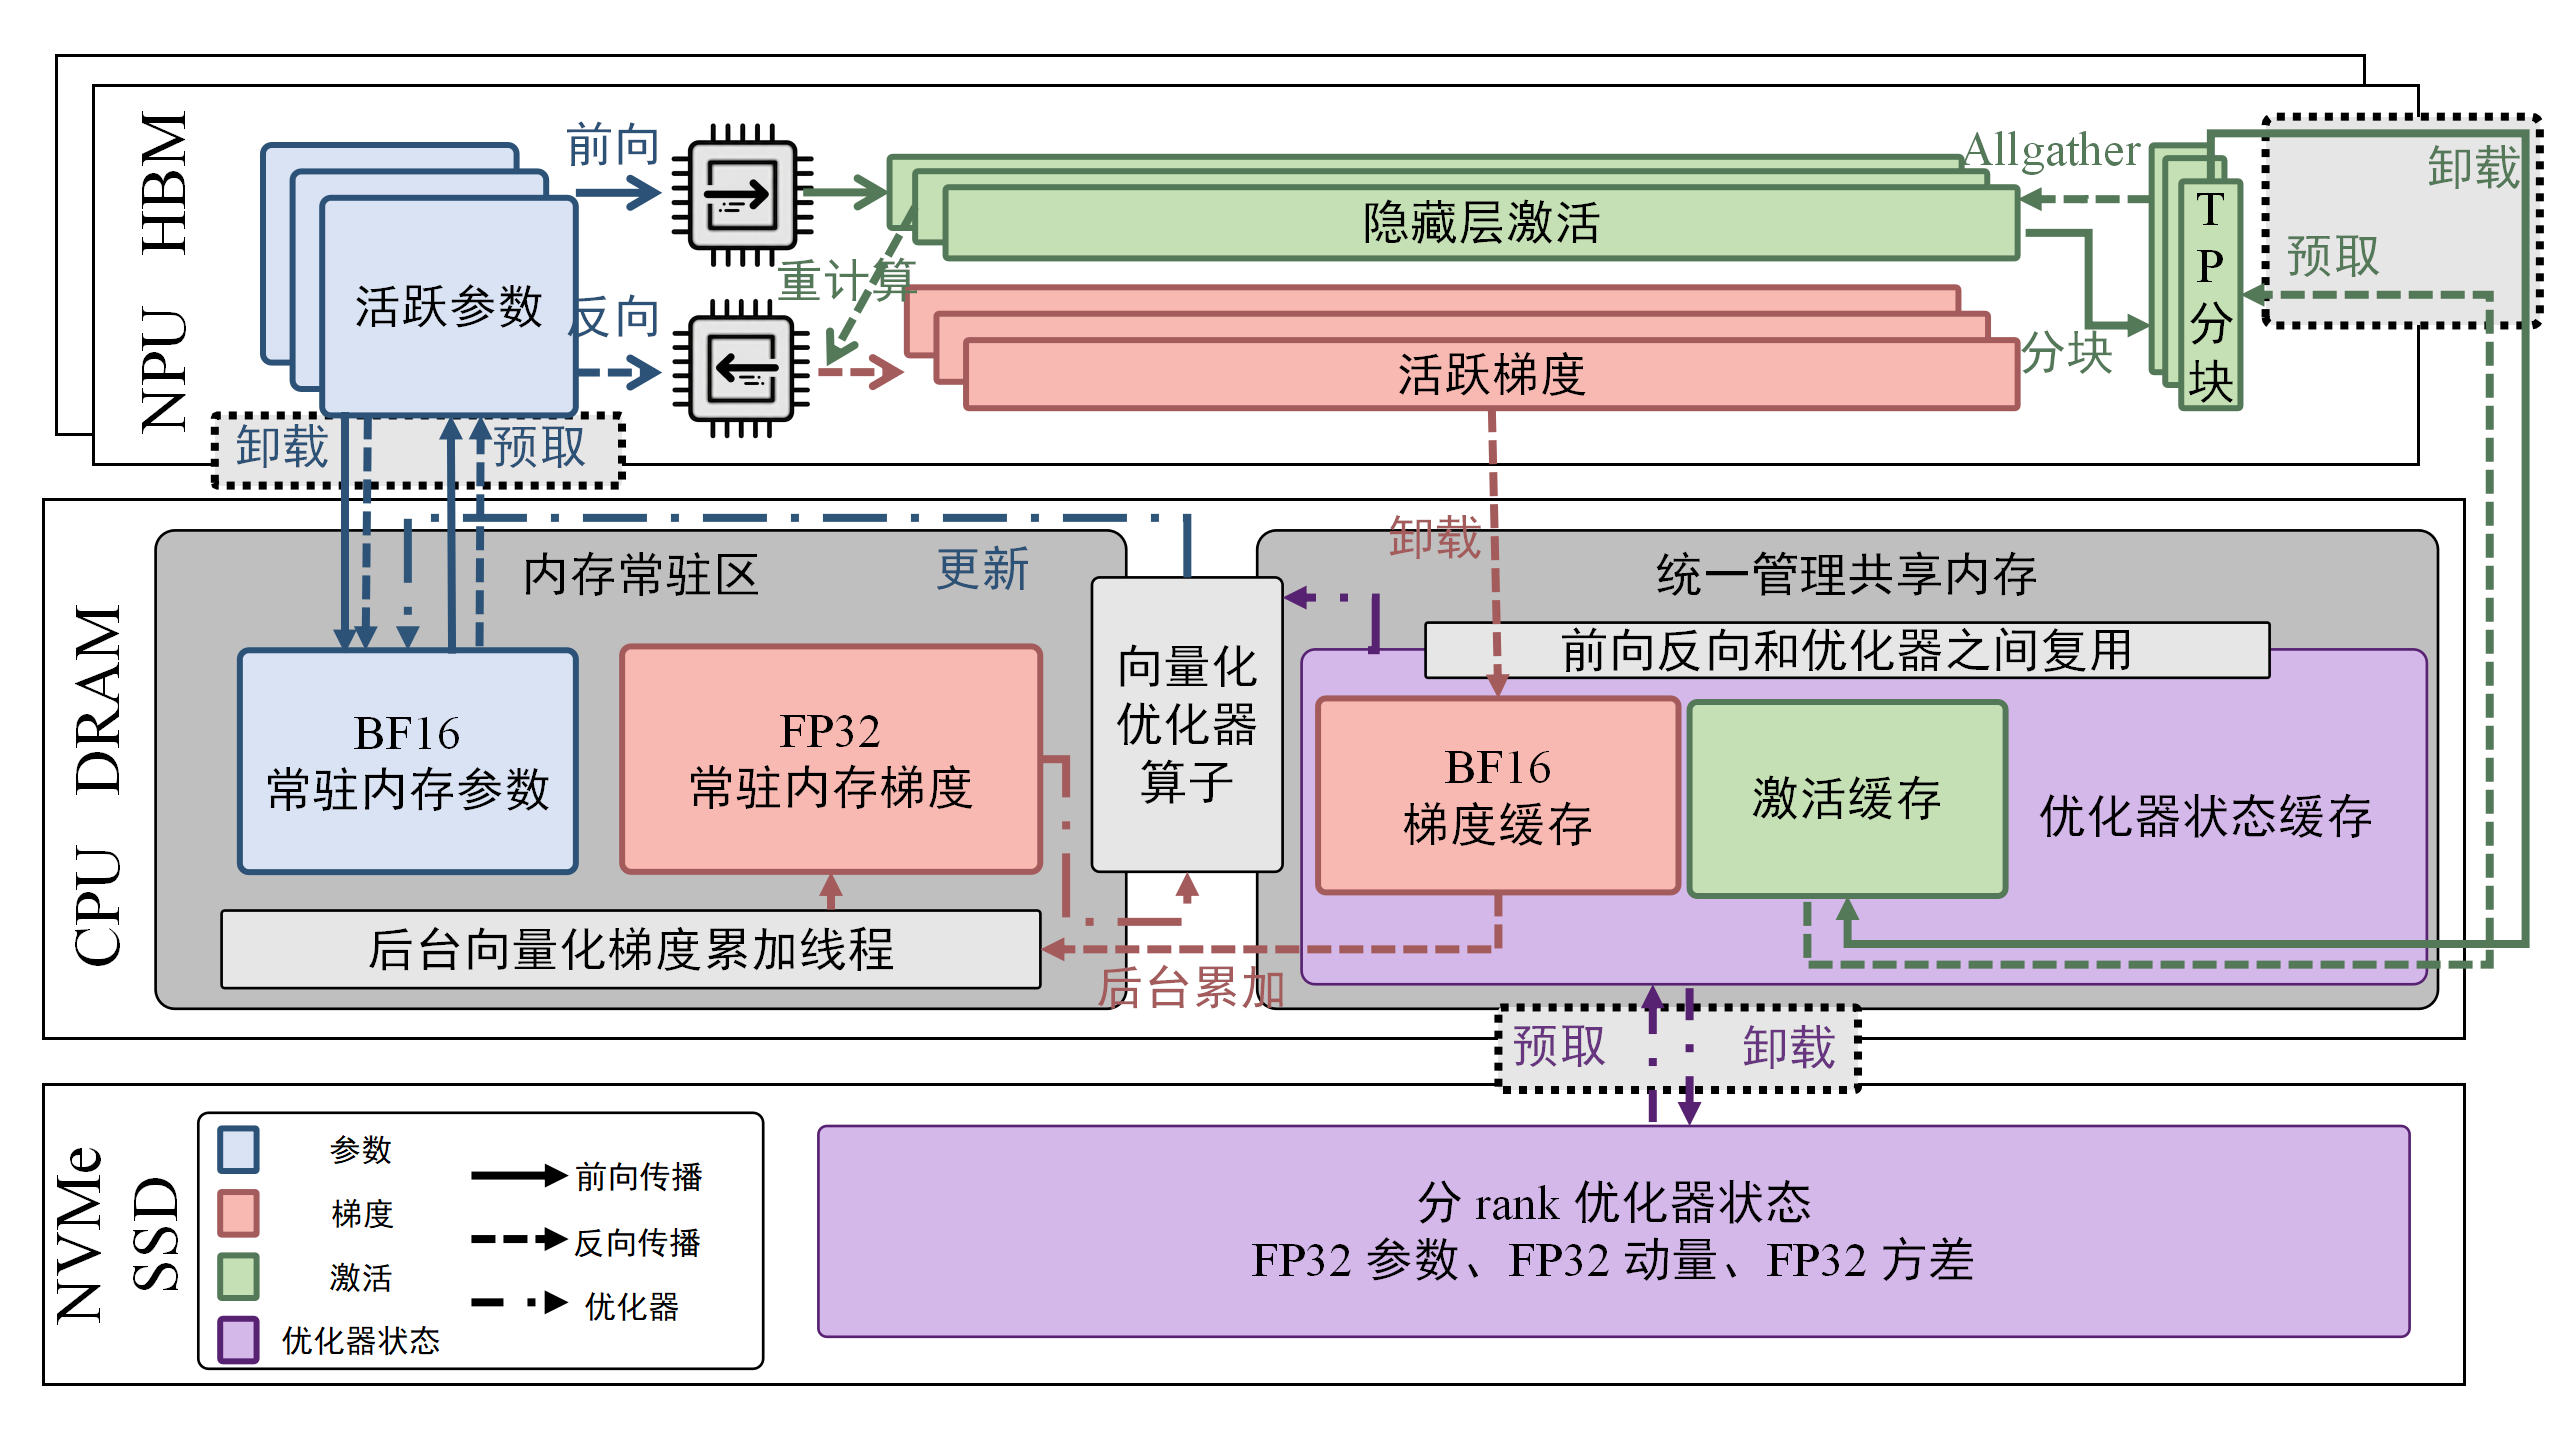
\includegraphics[width=1\textwidth]{figure/design.png}
  \caption{系统整体设计}
  \label{fig:sys-overall-design}
\end{figure}

对于模型参数，在混合精度训练场景下，
系统需要管理 BF16 和 FP32 两份参数，
其中 BF16 用于 NPU 前向和反向计算，
属于 NPU 需要频繁访问的张量。
系统在主机 DRAM 保存完整的 BF16 参数，
在 HBM 中仅保存活跃模块的参数副本。
而 FP32 参数不参与前后向传播，
作为优化器状态的一部分常驻于 NVMe SSD，
只在参数更新过程中被加载到 DRAM 工作区
完成更新，更新完成以后的 FP32 主参数再转换并
同步到 BF16 参数，从而保证前后向阶段使用的
BF16 参数和 FP32 主参数保持一致。

对于梯度，在梯度累加配置下，系统
维护 BF16 临时梯度和 FP32 主梯度。
其中 BF16 梯度是反向传播计算出来的临时结果，
FP32 主梯度用于跨批次累加。
考虑到梯度累加位于反向传播阶段，
需要避免 NVMe SSD 访问，因此 FP32 主梯度常驻在主机 DRAM 中。
反向传播计算得到的 BF16 梯度仅在 HBM 中临时存在，
随后被卸载到主机 DRAM 的 BF16 临时梯度缓冲中。
系统利用 CPU 侧的异构算力，
由 CPU 后台线程进行 BF16 到 FP32 的梯度累加，
累加完成后，CPU 侧的 BF16 临时梯度缓冲就可以复用。


对于激活值，系统开启全量重计算，
只保留 Transformer 层间的隐藏层，
这部分激活值还需卸载到主机 DRAM 中。
在某一层的反向阶段之前，
系统从主机 DRAM 恢复对应切片作为重计算输入，
其作用等价于前向阶段持续保留该层间隐藏状态。
在张量并行场景下，每个 rank 都持有一份完整的隐藏层，
为防止重复存储多份隐藏层导致内存占用过大，系统采用了分片缓存的方式，
每个张量并行 rank 都只持有隐藏层的一份切片。

对于优化器状态，其访问集中在参数更新阶段，
且总规模大于参与前后向计算的 BF16 参数。
系统将 FP32 主参数、一阶动量和二阶动量
切分为固定大小的数据块，并保存到 NVMe SSD 文件中。
主机 DRAM 仅提供当前状态块的工作区。
参数更新时，系统读入对应状态块，
结合 FP32 主梯度完成 AdamW 更新，
再将更新后的状态块写回 NVMe SSD。
这种分块组织在逻辑上等价于完整优化器状态常驻内存，
但物理上只要求少量块进入 DRAM。

\section{计算与 I/O 流水线设计}
根据前述张量生命周期和存储放置关系，
系统设计预取卸载流水线，使数据搬运尽可能与计算过程重叠。
本系统围绕训练过程中的张量迁移建立两条预取-
卸载流水线。第一条流水线为前向传播和反向传播时的计算-数据传输流水线，
连接 NPU 与 CPU，用于前向传播和反向传播阶段的参数、
激活与梯度迁移。第二条流水线为优化器计算时的优化器计算-数据 I/O 流水线，
连接 CPU 与 SSD，用于优化器状态管理。两条流水线共享主机侧缓冲层，
但面向不同类型的训练状态和不同的时间窗口，故
两条流水线可以按执行阶段独立组织。

前后向阶段的流水线以模块为基本调度粒度。
除了 embedding 层和输出层等少数边界模块外，
模型主体由多个同构的 Transformer 模块顺序堆叠而成，
同类 Transformer 模块具有相同的参数规模、张量形状和执行边界。
因此，不同模块可以共享同一套缓冲组织，
并在运行时执行序列中的相同相对位置触发数据迁移。
本系统前向和反向传播阶段的计算与数据传输流水线如图\ref{fig:npu-cpu-pipeline}所示。

该流水线只依赖运行时前后继关系，而不要求静态层号连续。
下文以 $m_k$ 表示运行时执行序列中的第 $k$ 个模块，
其编号只表示执行先后关系，可能与模型结构中的静态层号不同。
在普通前向传播中，执行序列通常与层号一致；
在反向传播中，执行序列与层号方向相反；
而在流水线并行或虚拟流水线并行中，
相邻执行模块还可能来自不同微批次或不同模型分块。

\begin{figure}[!htbp]
  \centering
  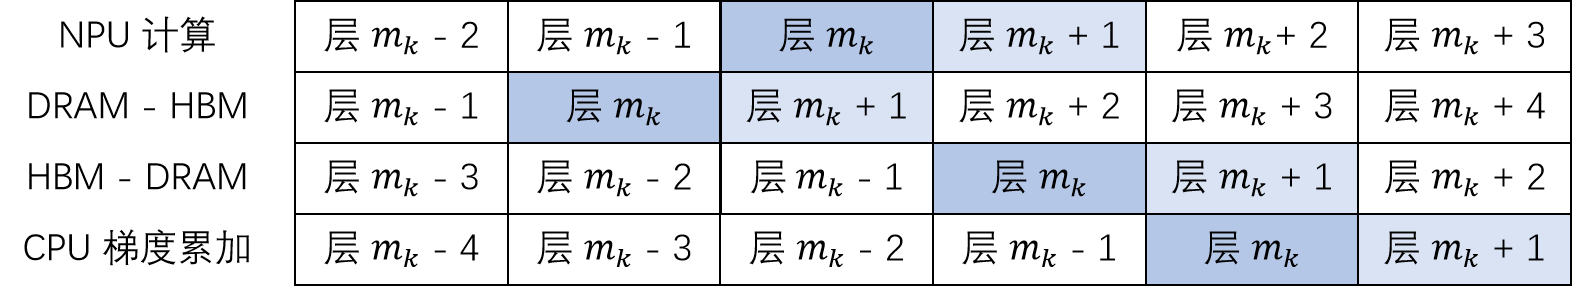
\includegraphics[width=1\textwidth]{figure/NPU_pipeline.png}
  \caption{前向反向传播计算-数据传输流水线}
  \label{fig:npu-cpu-pipeline}
\end{figure}

以当前计算模块为 $m_k$ 为例，
当 NPU 正在执行 $m_k$ 的前向或反向计算时，
主机到设备方向可以提前准备后继执行模块 $m_{k+1}$ 进入计算所需的设备侧张量；
设备到主机方向可以回收前驱执行模块 $m_{k-1}$ 已完成设备侧使用的张量；
在反向传播阶段，CPU 后台线程则处理更早完成卸载的 $m_{k-2}$ 的梯度累加。
由此，NPU 计算、主机到设备预取、设备到主机卸载和 CPU 梯度累加
在不同模块窗口上错位推进。

在该流水线中，数据通路与张量类型并非一一对应。
同一传输方向在不同训练阶段承担不同张量的迁移任务。
主机到设备方向主要承担后继模块参数预取，
以及反向重计算前的层间激活恢复；
设备到主机方向承担前向阶段的层间激活写出，
以及反向阶段 BF16 临时梯度的卸载；
CPU 梯度累加位于梯度卸载之后，
负责将主机侧 BF16 临时梯度转换并累加到 FP32 主梯度。


\begin{figure}[!htbp]
  \centering
  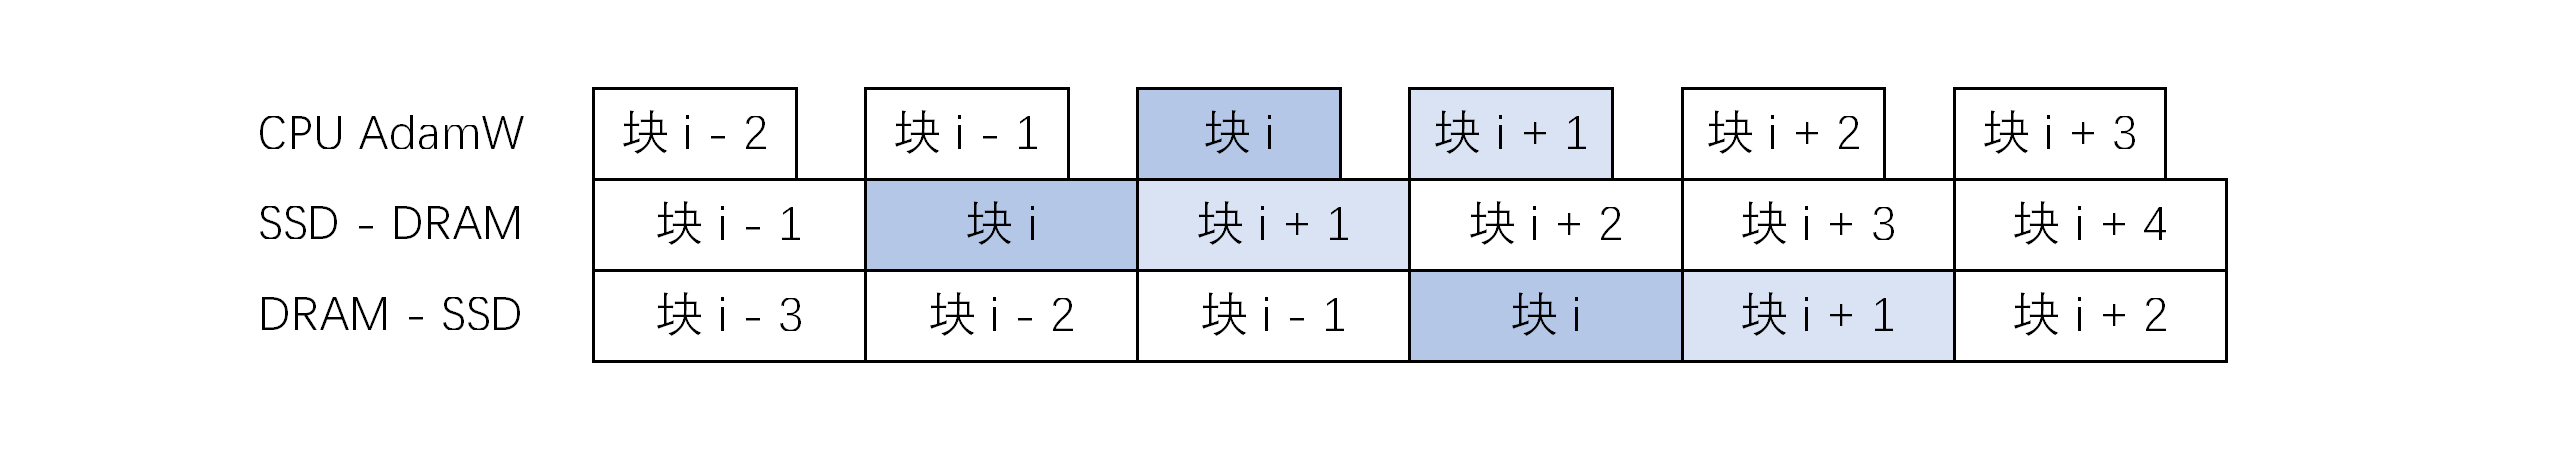
\includegraphics[width=1\textwidth]{figure/optim_pipeline.png}
  \caption{优化器阶段计算IO流水线}
  \label{fig:optimizer-io-pipeline}
\end{figure}

CPU 与 SSD 之间的流水线主要对应优化器更新阶段，管理优化器状态。
系统将主参数、一阶动量和二阶动量按照数据块组织，
并存放在 SSD 中。每次进入参数更新阶段时，
系统先将当前数据块对应的状态从 SSD 读入 CPU 侧缓冲区，
随后结合当前块对应的梯度数据在 CPU 上执行更新，
再将更新后的状态写回 SSD。优化器状态无需全部驻留在主机内存，
只需要以数据块为单位滚动进入工作区。

该分块流水线的可行性来源于优化器更新的逐元素特征。
以 AdamW 为例，主参数、梯度、一阶动量和二阶动量
在相同位置上的元素共同决定该位置的更新结果，
不同位置之间不存在数据依赖。
因此，在学习率、权重衰减等优化策略相同的参数组内部，
更新计算不依赖张量原本所属的网络层或参数对象边界。
系统可以将同一参数组内连续范围的状态合并为数据块，
交由同一个 CPU 算子完成更新。
这种组织方式既保持了优化器语义，
又使 SSD 读写和 CPU 更新能够以连续数据块为单位推进。
优化器阶段的计算与 I/O 流水线如图\ref{fig:optimizer-io-pipeline}所示。


% 流水线需要记录完成条件，进行同步控制。对于设备与主机之间的路径，
% 参数未完成准备时不得进入对应模块计算，参数、
% 激活未完成恢复时不得进入重计算阶段，
% 同时激活或者梯度未卸载完成时原有的缓冲区不得被新的数据覆盖。
% 对于主机与 SSD 之间的路径，状态未完成读取时不得进入更新，
% 更新结果未完成写回时工作槽不得复用。
% 本系统在 NPU-CPU 侧主要通过 Torch Event 进行同步控
% 制，
% 在 CPU-SSD 侧通过异步 IO 系统调用结果进行控制。

\section{NPU HBM 管理与缓冲调度}
为了实现上述 NPU 模块粒度的参数驻留控制和预取卸载流水线，
系统在 NPU 侧对 HBM 进行管理，通过设置缓冲槽保证数据正确性。
系统按模块类型组织缓冲槽。
其中主体 Transformer 模块数量多、结构一致，
是槽位复用的主要对象；
embedding 层和输出层等边界模块则作为独立类型处理。
每类模块在初始化时在 NPU 上申请固定数量的缓冲槽，
作为运行时活跃参数及相关临时张量的设备侧物理位置。
在运行时，模块参数随着执行过程动态加载到所属类型对应的 NPU 槽位中；
当模块离开活跃窗口后，其占用的槽位即可释放或复用。

NPU 侧槽位管理与复用过程如图\ref{fig:npu-slot-mgmt}所示。

\begin{figure}[!htbp]
  \centering
  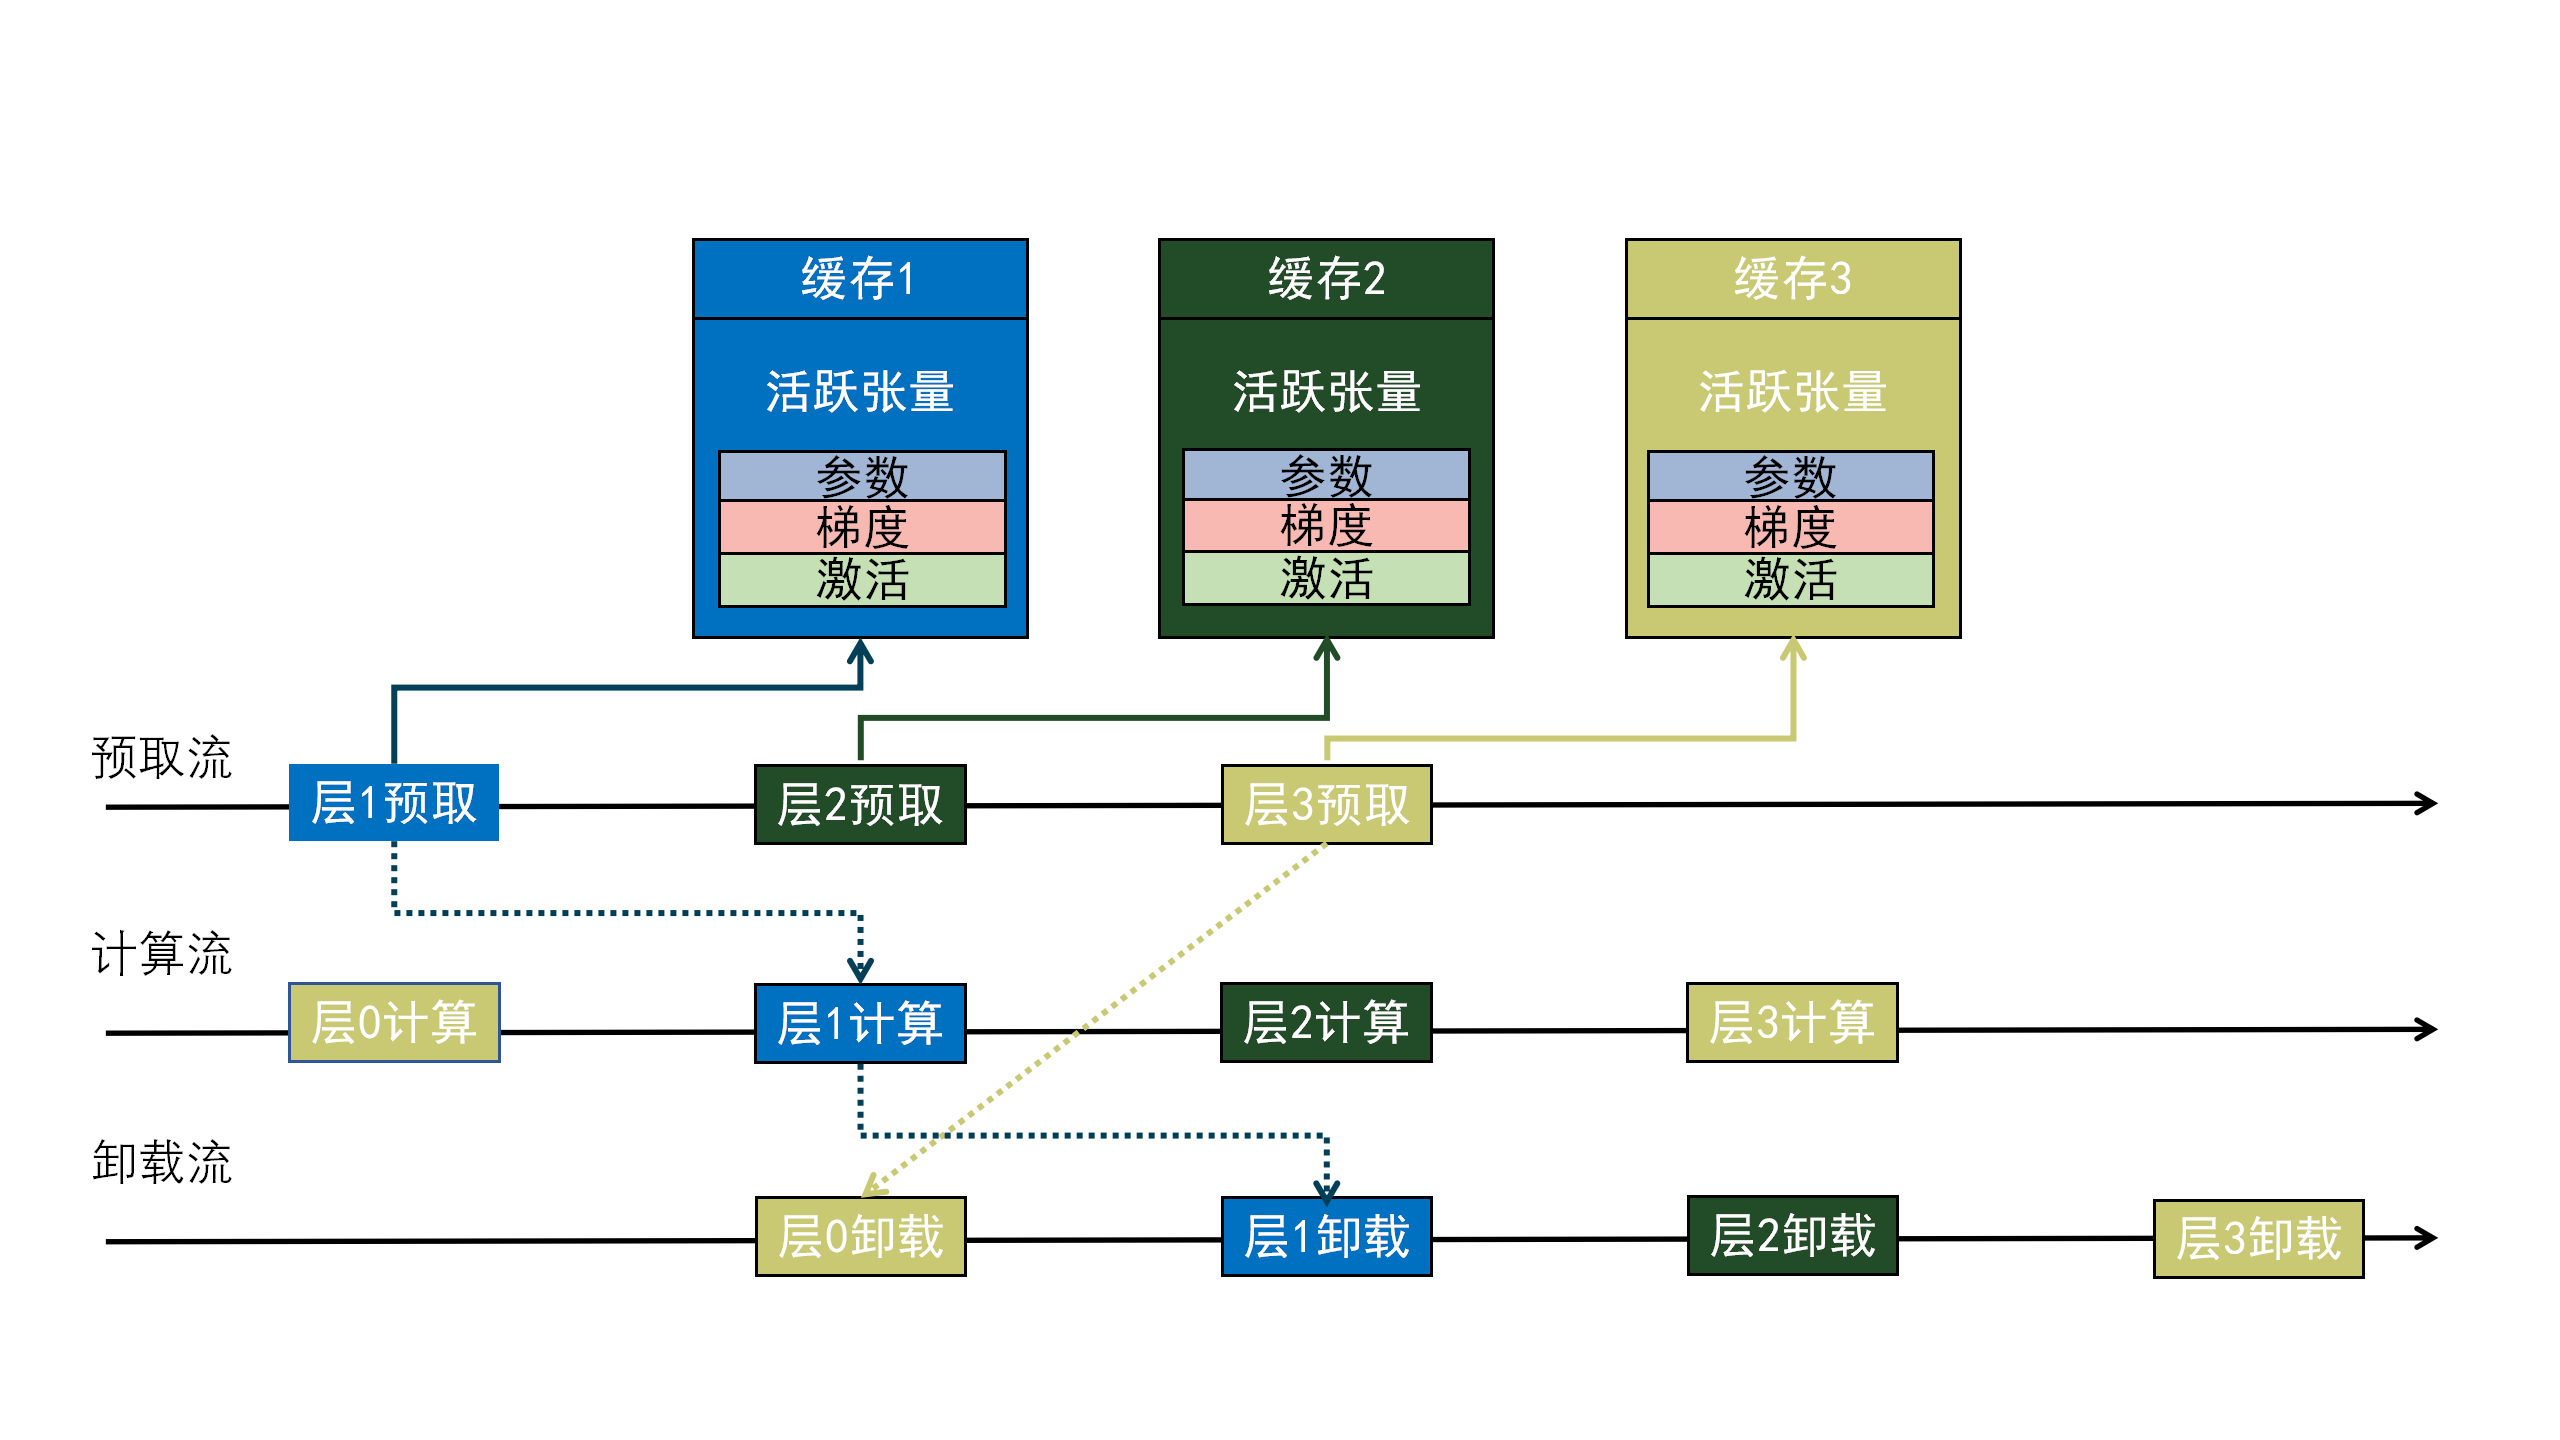
\includegraphics[width=1\textwidth]{figure/NPU_slot.png}
  \caption{NPU HBM 管理示意图}
  \label{fig:npu-slot-mgmt}
\end{figure}

缓冲槽数量决定了 HBM 占用和流水线重叠能力。
前后向阶段的设备侧流水线主要由预取、计算和卸载三个阶段组成，
槽位数量只需要覆盖这些同时活跃的阶段。
如果继续增加槽位，
虽然可以保留更多模块的设备侧副本，
但不会引入新的计算或传输阶段，
因此也难以进一步提高计算与传输的重叠程度。
同时更多槽位还增加了 HBM 常驻占用。
如果槽位数量过少，
预取、计算和卸载三个阶段
无法同时执行，会导致数据传输不充分掩盖。
因此，系统采用三个可复用槽位，
同步支撑预取、计算和卸载阶段的执行。

为了正确索引模块对应的参数在主机内存和 NPU 槽位上的位置，
系统在初始化时注册模块在本 rank 中的全局编号，
通过模块管理器索引模块在主机内存上的位置，
并在运行时动态维护模块编号和 NPU 槽位的映射关系。

在运行时，引擎需要保证 NPU 槽位的持续复用，
为此需要正确追踪模块的生命周期，并在合适的时机进行预取和卸载。
系统采取了多流和事件等待的方式进行控制。NPU 分为预取流、
计算流和卸载流，分别负责模块状态的 DRAM 到 HBM 异步复制、
模块计算和 HBM 到 DRAM 异步复制。例如，当模块 $m_k$ 开始计算前，
系统可以提前准备后继模块 $m_{k+1}$ 的预取；
在执行预取前，需要确认目标槽位上的旧模块已经完成计算和必要卸载，
防止新数据覆盖仍在使用的数据；
$m_{k+1}$ 开始计算前，
则需要等待其参数完成设备侧准备。

（TODO-AI：
从状态上看，每个槽位是模块活跃窗口内设备侧张量的临时物理位置，
在空闲、预取中、可计算、计算中、卸载中和可复用等状态之间转换。
预取流只能写入空闲或可复用槽位，
计算流只能读取已经完成预取的槽位，
卸载流只能处理计算完成且后续不再使用的槽位。
这些状态约束保证同一槽位不会被多个阶段同时写入或读写冲突。）

缓冲调度采用 LRU 机制记录最早调入且已满足复用条件的 NPU 槽位。
每当预取模块被调入某一槽位时，
调度器更新该槽位的最近使用状态。
后续需要选择预取目标时，
调度器优先选择最早调入且已满足复用条件的槽位。
在复用前，系统等待该槽位对应模块的计算和卸载完成，
再执行主机内存到 HBM 的预取。
该机制保证了执行流水线中逐个模块都能尽快执行预取和计算。

（TODO-AI：
该策略适用于 Transformer 模块的顺序访问特征。
在局部执行序列中，较早调入的模块通常也较早失去继续驻留价值。
因此，选择最早调入的可复用槽位，
可以用较低的状态维护开销近似获得顺序执行下的复用效果。）



\section{主机共享内存管理}
系统在主机侧采用共享锁页内存管理所有缓存，包括BF16参数缓存、
FP32主梯度缓存、激活缓存、BF16临时梯度缓存以及优化器状态临时缓冲
区。
该内存区域为连续底层存储，在其上根据不同用途构造多个张量视图，
并为不同缓冲区设置独立布局。该设计下多类张量共用同一块主机内存资源，
同时减少了运行过程中的重复分配与回收，降低了微调过程中内存碎片化的风险。

该共享内存区域分为独占区和共享区域两部分，
独占区要求在微调全过程不能被其他部分复写，需要保证数据完整性，
主要管理 BF16参数和FP32主梯度；
共享区则用于临时缓冲，这部分张量只在一段运行时生命周期内有效，
生命周期前保证先写入，不会读取脏数据，生命周期结束后即可被其余缓存覆盖，
且不同张量可以分为生命周期互不交叉的组，主要管理激活缓存、
BF16 临时梯度缓存和优化器状态临时缓冲区。
该设计主要目的在于压缩临时缓冲区的大小，
节省主机内存的占用以提升可微调规模。

在临时缓冲中，本系统将张量分成前后向传播和优化器两部分生命周期不交叉的组
。BF16临时梯度和激活值归属前后向传播组，
因为它们只活跃于前后向传播流程。BF16临时梯度在某模块反向传播结束时产
生，并由 CPU 算子累加到 FP32 主梯度区域，随即生命周期结束；
而激活值在前向传播时产生，反向传播时消费，随即生命周期结束。
而优化器状态在优化器执行时被临时
调入到 CPU 内存中，
参数更新后即持久化到 SSD 中，并同步到 BF16 参数，
故只活跃于优化器计算阶段。
这两个时间阶段互不交叉，两者共用同一片内存区域。
主机侧共享内存分区与生命周期管理如图\ref{fig:cpu-shared-mem}所示。

\begin{figure}[!htbp]
  \centering
  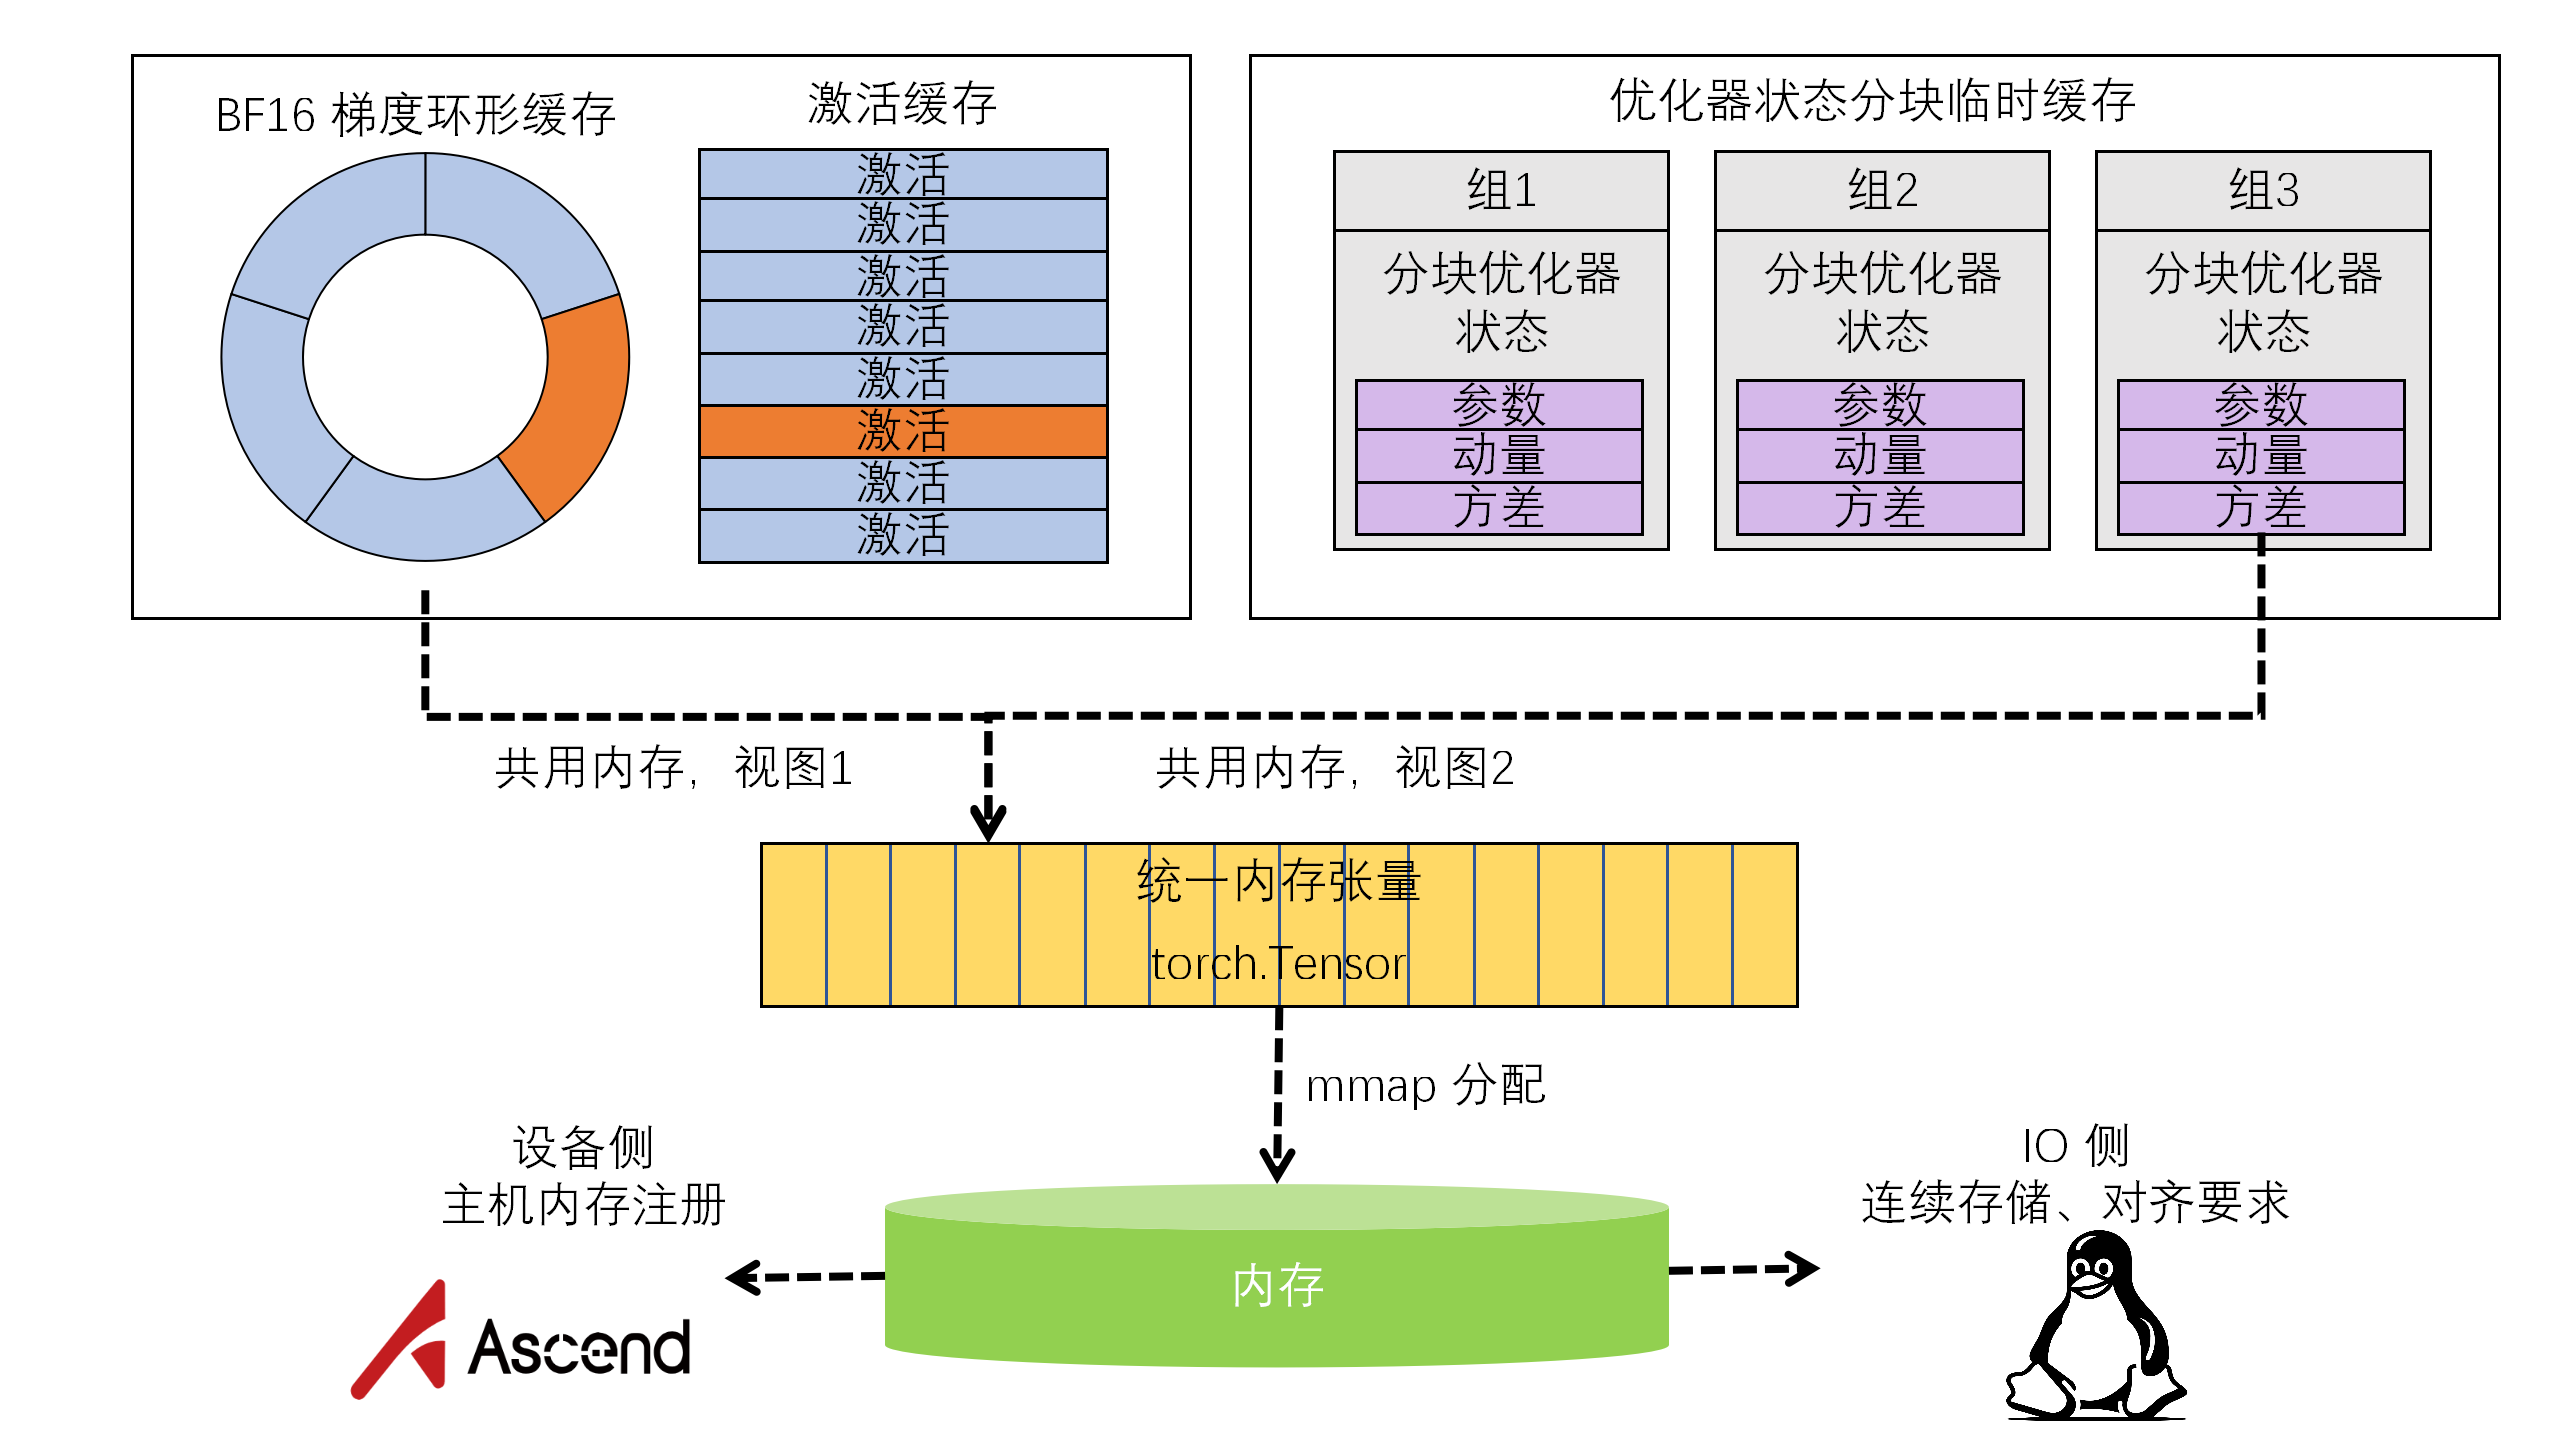
\includegraphics[width=1\textwidth]{figure/share_mem_manager.png}
  \caption{CPU 共享内存管理}
  \label{fig:cpu-shared-mem}
\end{figure}

共享内存以 torch tensor 为界，分为物理层和逻辑层两层。
在物理层，张量需要同时满足对齐管理和锁页功能。
这是由于主机侧缓冲区既服务于设备与主机之间的张量搬运，
也服务于主机与 SSD 之间的直接 I/O。
因此在昇腾 NPU 侧需要保证其为锁页内存，
通过 aclrtHostRegister 将其注册为锁定页，
该操作保证其不会被操作系统换页，从而能够执行非阻塞的
异步拷贝，
保证前后向过程中可以进行异步的预取和卸载。在文件系统IO侧，
为了高效IO和减少页缓存对内存的占用，
系统采用 \texttt{O\_DIRECT} 模式读写文件，
这要求优化器状态缓冲张量的地址基址和块大小满足对齐条件。
系统在分配阶段对缓冲区大小、
起始偏移和地址边界施加约束，使张量能够满足直接 I/O 的访问要求。

在逻辑层，激活值、梯度临时缓冲和优化器状态缓冲都
以 torch 张量形式进行组织。
其中系统用（模型分块编号、块内编号、微批次数）三元组索引激活值在主机内存中的位置，
在前向时动态申请激活缓冲块，在反向使用完成后即释放；
用环形缓冲区进行管理 BF16 梯度，当NPU反向计算完成时
申请梯度临时缓存，
并由 CPU 累加算子累加到主梯度，累加完成即可释放。
而优化器缓冲结合优化器的线性读写以及逐元素计算的特点，
用固定大小分块的管理方式，
每个块包括主参数、动量和方差，在运行时从 SSD 载入、计算并写回。

\chapter{系统实现}

\section{系统架构}
本系统基于 Megatron-MindSpeed 训练框架实现，
所用的版本为 \texttt{Megatron-core 0.12.1} 和 \texttt{Mindspeed core\_r0.12.0}。
系统实现了多级存储管理逻辑，
将运行时引擎插入框架原有的分布式训练主流程。
整个系统架构可分为四个层次。第一层为训练框架层，
负责模型前向传播、反向传播执行过程以及 TP、DP、PP、
VPP 等分布式并行策略。其中 DP 能力由原 Megatron-MindSpeed 框架保留，
本文调度设计主要面向 TP、PP 和 VPP 下的执行序列。
上述框架层由 Megatron-MindSpeed 框架开源代码
实现。第二层为运行时引擎层，
通过对框架少许修改和自定义模块的引入，实现参数、激活、
梯度和优化器状态的生命周期管理和迁移时机控制。第三层为存储管理层，
实现各类缓存的布局与索引管理，包括共享锁页内存管理以及与昇腾运行时和操作系统的桥接，
同时包含一些附属计算组件，如重新实现的算子。
第四层则为硬件，包含昇腾 NPU 910B，鲲鹏 CPU，NVMe SSD
以及 PCIe HCCL 等通信组件。

如图\ref{fig:impl-arch}所示，
训练框架层和异构硬件层由既有框架与硬件平台提供，
本工作实现其中的运行时引擎层和存储管理层。
\begin{figure}[!htbp]
  \centering
  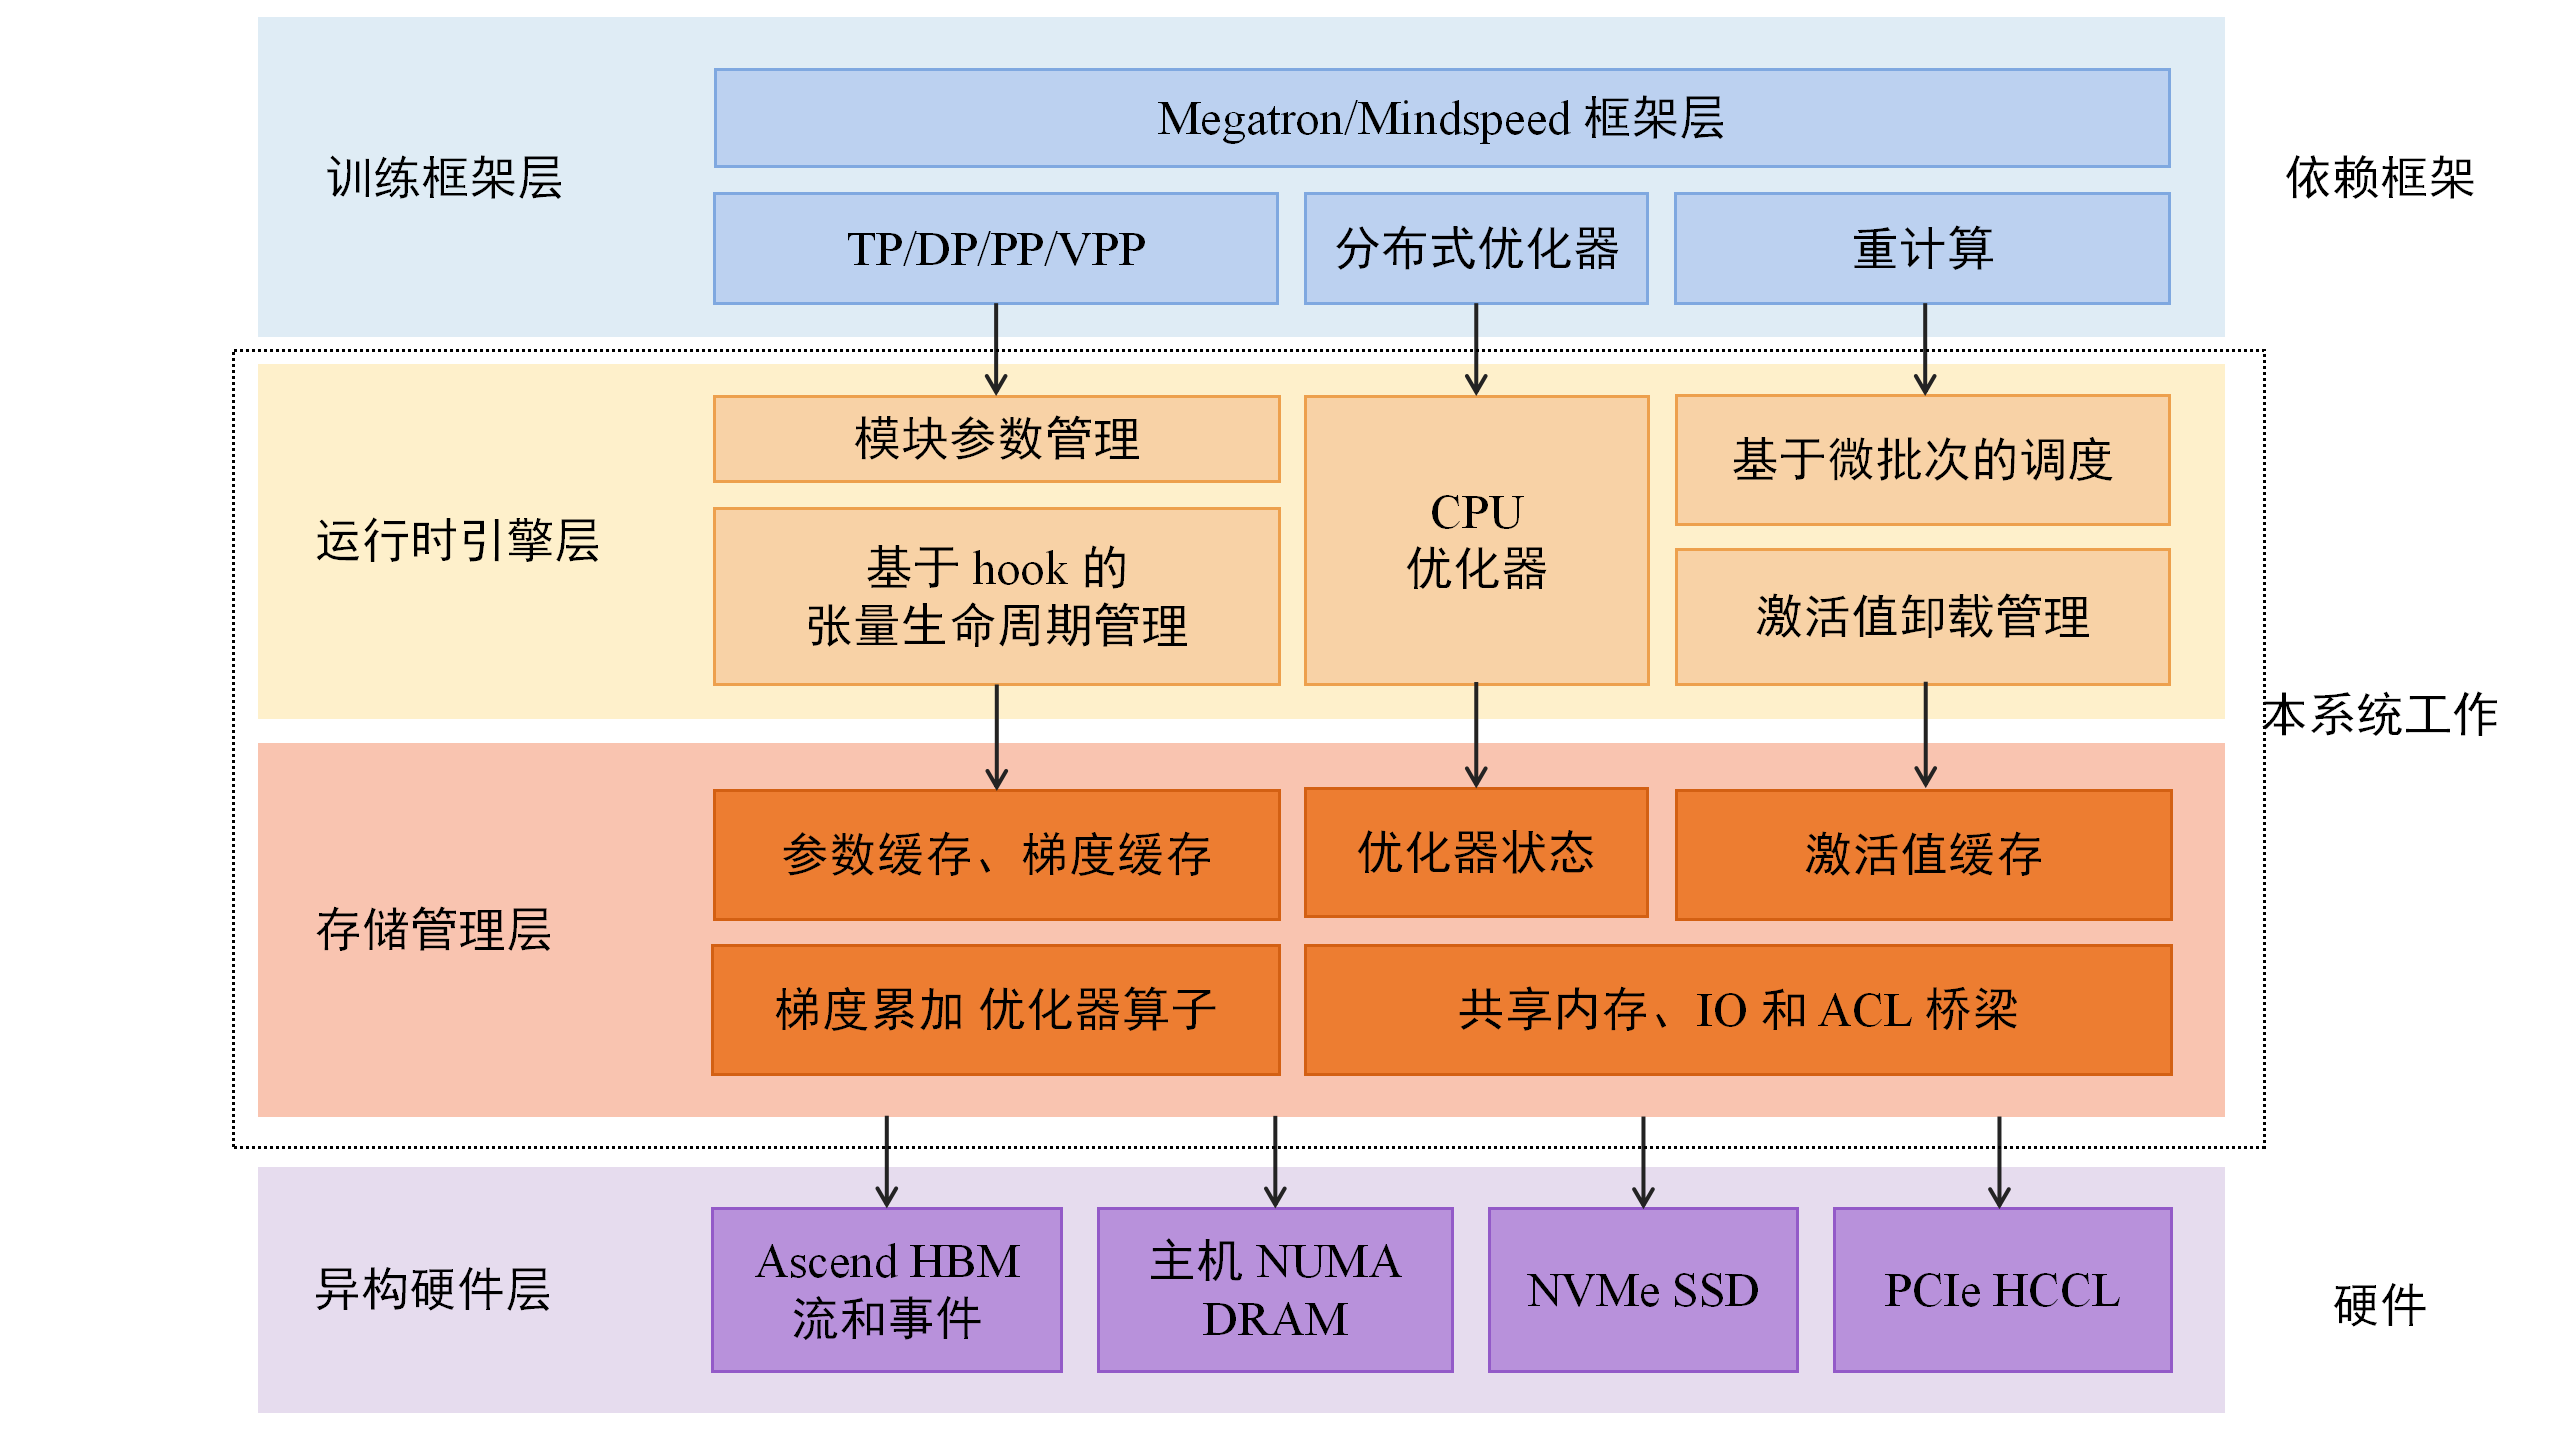
\includegraphics[width=1\textwidth]{figure/soft_design.png}
  \caption{系统实现架构图}
  \label{fig:impl-arch}
\end{figure}

存储管理层管理了常驻的参数缓存、梯度缓存、激活值缓存
和优化器状态。
其中参数缓存和梯度缓存常驻于主机 DRAM，
为运行时引擎提供可按模块和参数访问的主机侧张量视图。
两类缓存通过模块编号和参数段位置被运行时调度模块索引。
激活值缓存活跃于前向传播到重计算阶段之间，
以模型分块、局部层位置和微批次标识索引，
在多个微批次交错执行时能定位正确的 Transformer 层间隐藏状态。
优化器状态常驻于 NVMe SSD。
其为主参数、动量和方差组成的可顺序处理的数据块。
参数更新时，运行时引擎可以按块取得对应状态和梯度。

共享内存、I/O 和 ACL 桥梁是存储管理层的底层接口。
它向上提供统一的主机缓冲分配和张量视图，
向下连接昇腾运行时与文件 I/O，
使主机侧的参数、梯度、激活和优化器工作区共用同一套
注册内存分配与异步 I/O 机制。
梯度累加和优化器算子属于存储管理层中的计算组件，
用于对连续缓冲执行主机侧数值计算。

运行时引擎层包括模块参数管理、基于钩子的张量生命周期管理、
基于微批次的调度、激活值卸载管理和 CPU 优化器等子模块。
模块参数管理模块在初始化阶段扫描并登记被管理模块，
建立模块、参数缓存和 NPU 槽位之间的运行时关系。
微调过程中，该模块根据执行序列选择需要加载或回收的模块参数，
并更新模块在设备侧的驻留状态。
基于钩子的张量生命周期管理在框架模块边界触发这些操作，
使张量预取、卸载和等待随前向或反向执行过程自动触发。
基于微批次的调度处理流水线并行和虚拟流水线并行下
执行序列与静态层号不一致的问题。
其根据流水并行顺序，
以微批次、模型分块和局部层位置三元组标记运行时执行顺序。
激活值卸载管理与重计算流程配合，
负责层间激活在前后向之间的保存与恢复，
不改变框架重计算本身的语义。
CPU 优化器在参数更新阶段接管主机侧优化器计算，
并调用存储管理层提供的优化器状态块和算子接口完成更新。

\section{基于 pytorch hook 机制的运行时引擎}
PyTorch 为 nn.Module 提供了模块级的回调接口，分别叫做
\texttt{forward/backward\_prehook/hook}，下面统称为钩子。
钩子可以注册在 \texttt{nn.Module} 对象上，
在该模块执行到相应阶段时钩子定义的操作由 Pytorch 触发。
本文使用 PyTorch 提供的以上钩子接口，
将运行时引擎嵌入原始框架的微调流程中，
在不改写层内模块的前提下，
把参数的预取和释放、梯度的卸载等张量管理逻辑插入了模块执行边界。

四类钩子的触发位置、回调签名和系统操作如表\ref{tab:pytorch-hook-api} \upcite{pytorch_module_hooks}所示。

\begin{table}[!htbp]
\centering
\caption{本文使用的 PyTorch 模块钩子接口}
\label{tab:pytorch-hook-api}
\begin{tabular}{p{0.32\textwidth}p{0.25\textwidth}p{0.33\textwidth}}
\toprule
接口 & 回调签名 & 系统操作 \\
\midrule
\texttt{register\_forward\_pre\_hook}
& \texttt{hook(module, args)}
& 执行前序反向传播卸载，预取后继模块参数、梯度并等待当前参数准备完成 \\
\texttt{register\_forward\_hook}
& \texttt{hook(module, args, output)}
& 执行卸载并更新当前模块参数驻留状态 \\
\texttt{register\_full\_backward\_pre\_hook}
& \texttt{hook(module, grad\_output)}
& 执行前序反向传播卸载，预取后继模块参数、激活并等待当前参数与梯度临时区域准备完成 \\
\texttt{register\_full\_backward\_hook}
& \texttt{hook(module, grad\_input, grad\_output)}
& 记录后续需要执行的卸载操作 \\
\bottomrule
\end{tabular}
\end{table}

系统在初始化过程中会首先遍历每个模型块中的嵌入层、各解码层、
最终归一化层和输出层，将这些模块登记到统一的参数管理器，
再在这些目标模块上注册四类回调。在记录模块的同时登记每个模块的全局索引和
分块局部索引，分别用于后续参数和激活值在任一回调中直接定位
张量在内存中的位置。

前向或反向的入口钩子执行和预取卸载工作，并完成进入模块计算前的参数准备。
当前模块开始计算前，系统根据当前模块、
传播方向和微批次确定本次执行在运行时序列中的位置，
并进一步得到前一个执行目标和下一个执行目标；
随后卸载前一个执行目标的参数和梯度，
并对下一个执行目标启动参数预取；
最后等待当前模块自身的参数加载完成。

运行时序列由训练框架层并行配置确定。
当流水线并行度为一时，
本 rank 只包含一个模型块，
序列由同一微批次上的前向阶段和反向阶段顺序排列而成。
当启用流水线并行或虚拟流水线并行时，
同一 rank 会交错执行不同模型块和不同微批次，
因此序列项由阶段、模型块编号和微批次编号共同表示。
系统在初始化阶段可以构建出执行序列，
并维护一个指向当前序列项的游标。
钩子触发时，
模块参数管理单元根据初始化列表取得当前模块对应的模型块编号和块内局部位置；
若后继目标仍在同一模型块内，
则由块内局部位置确定相邻模块；
若当前模块已经位于模型块首尾，
则由下一序列项确定后继模型块、微批次以及该阶段对应的起始模块或末尾模块。
即前向顺序执行、反向逆序执行以及 PP/VPP 下的交错执行
可以统一表示为运行时序列上的相邻目标查询。

前向出口钩子更改当前模块前向结束后的参数驻留状态。
系统在该位置再次查询后继目标。
只要后一个执行任务不使用当前模块参数，
则启动当前模块参数卸载。
反向出口钩子处理反向阶段后的卸载记录。
由于反向阶段可能包含重计算过程，
系统不在反向出口位置直接进行卸载，
而是记录待卸载模块，
在后续入口钩子或训练步末尾执行实际卸载。
由于反向出口钩子不实际执行卸载，系统还需在训练步末尾设置统一卸载，
完成最后一轮参数卸载和梯度卸载，并等待后台梯度累加任务结束。

上述参数和梯度迁移都可以由模块级钩子覆盖，
而层间激活的保存和恢复发生在重计算检查点函数中，
在训练框架层的原始实现中使用了 \texttt{save\_for\_backward} API 将激活保存在 HBM 中，
而本系统的设计中，其需要卸载到主机 DRAM 中，
因此本系统需要对框架实现进行修改，
对检查点函数进行重新封装。
在进入检查点函数时记录当前模型块、
局部层位置和微批次编号，以便上述钩子函数进行主机内存的缓存定位。

前向阶段，系统在检查点路径保存 Transformer 层间的激活，
并将其写入主机侧缓存。缓存完成后，设备侧不再通过
\texttt{save\_for\_backward} 保留这一部分隐藏层激活值。

反向阶段，系统在进入对应检查点段的重计算前，先确认激活已经由
预取模块拷贝到设备侧，等待该拷贝完成。
随后进入重计算路径，重新执行该段前向，再继续完成梯度传播。
激活缓存使用后立即释放。系统在对应重计算和梯度传播结束后，
将该缓存块归还到主机侧缓冲池，用于后续微批次或其他模型块复用。

以上所有 NPU 和主机侧的数据拷贝都使用 torch 张量的 \texttt{copy\_} API，
同时开启非阻塞选项，保证拷贝过程不阻塞调度进程的执行，从而实现
数据传输和计算的重叠。


\section{基于事件的流同步}

本系统将参数预取、梯度卸载、激活迁移和梯度累加放在不同流乃至
不同设备中并发执行。
这意味着不同操作的实际执行顺序可能不同于发射顺序，
操作所依赖的前序任务不一定在自身启动前完成。
因此，系统需要在张量被读取、覆盖或复用之前建立完成条件，
并进行流和线程之间的同步。

本设计中的同步实现分为两类。
一类用于 NPU 参数槽位和激活缓冲的流间同步，
另一类用于 CPU 后台线程与主线程之间的跨线程同步。
前一类由常规流事件完成，
用于描述加载流、卸载流和计算流之间的先后关系；
后一类由主机侧任务完成句柄表示，
用于描述主机后台线程任务是否已经结束。
系统利用这些完成条件，
保证各种张量在被读取或复用前已经完成上一阶段操作。

系统围绕张量状态和缓冲复用关系维护若干事件组。

参数加载事件组描述主机参数到设备参数槽位的完成状态。
参数预取在加载流中执行。
每次预取完成后，
系统以模块、传播阶段和微批次为键，
记录对应的加载完成事件。
前向入口和反向入口在计算流上等待该事件，
随后才允许当前模块读取对应参数。
该同步事件组保证计算开始前所有参数已经准备就绪。

槽位复用事件组描述 HBM 参数槽位何时可以被后续模块覆盖。
系统为每个参数槽位维护计算完成事件和梯度相关完成事件，
分别记录计算流结束和梯度卸载结束。
当某一模块离开设备侧驻留状态时，
系统把当前计算流上的完成事件和卸载流上的完成事件记录到槽位元数据中。
后续预取流如果使用同一槽位，
需要在异步拷贝执行前等待这两个事件。
该同步事件组保证新模块参数不会覆盖仍被计算流读取的旧参数，
也不会覆盖仍在卸载流读取的梯度或参数数据。

梯度拷贝事件组描述设备侧临时梯度写入主机缓冲的完成状态。
反向卸载时，
系统先在卸载流中把 BF16 梯度写入主机临时缓冲，
并记录梯度拷贝完成事件。
CPU 后台线程在启动累加前等待该事件，
从而保证读取到的临时梯度已经完整写入主机内存。

任务完成句柄约束主机侧 BF16 临时梯度缓冲在累加之后的复用。
梯度拷贝完成后，
CPU 后台线程执行 BF16 到 FP32 主梯度的累加。
每个临时梯度缓冲同时保存一个任务完成句柄。
当后续梯度再次申请到同一缓冲时，
运行时引擎层用于发射设备侧算子的主线程
先阻塞等待上一轮后台累加完成，
再发射新的 BF16 梯度从设备到主机的异步拷贝任务。
训练步末尾主线程统一等待全部后台累加任务对应的完成句柄，
保证本轮反向传播产生的梯度已经合并到主梯度中。

优化器 I/O 完成句柄描述 SSD 状态块与主机工作区之间的依赖。
优化器状态以块为单位在 SSD 和 DRAM 工作区之间迁移。
每个优化器工作槽维护 I/O 完成句柄列表，
用于保存优化器状态读请求和状态写回请求的完成句柄。
在工作槽被再次使用前，
系统统一等待并清空该列表。
该事件组确保 CPU 优化器算子只会访问已经完成读取的状态块，
新的状态块也不会覆盖尚未写回 SSD 的更新结果。

在资源受限训练场景中，
每一层和每个微批次都会产生拷贝完成事件或后台任务完成标记。
如果每次迁移都重新创建事件对象，
会增加运行时开销并扩大事件资源占用，
在模型规模和微调轮次极大时会出现事件资源耗尽的错误，
导致微调不能够稳定完成。
因此，系统对事件采用池化管理。
梯度拷贝完成事件由拷贝事件池管理，
系统按照尾指针顺序取用已有事件，
池中不足时才创建新事件。
在一个微调轮次结束时，
系统会清空参数加载事件、
激活预取记录和槽位中的完成事件，
并重置事件池尾指针。
这一机制使事件对象数量随单步最大并发需求增长，
而不会随着训练迭代次数持续增加。

\section{面向异步拷贝与直接 I/O 的注册主机内存实现}
第三章已经从设计层给出了主机共享内存的分区方式和生命周期复用策略。
本节进一步说明该内存区域在系统实现中的访问入口：
同一块主机内存既要作为 torch 张量参与 NPU 与主机之间的异步拷贝，
又要作为直接 I/O 缓冲区参与主机与 NVMe SSD 之间的数据交换。
普通 PyTorch \texttt{pin\_memory} 张量主要面向设备拷贝，
不能同时保证直接 I/O 的页对齐、连续大块切分和跨线程复用管理；
在直接作为 SSD 读写缓冲时，
会因地址或长度不满足对齐要求而触发 EFAULT 错误。

为此，系统在 C++ 扩展中实现注册主机内存入口。
初始化时，系统首先通过 \texttt{mmap} 申请一段连续主机虚拟内存，
再按照直接 I/O 的最大对齐约束调整可用区域的起始地址和长度。
完成对齐后，
系统调用 \texttt{aclrtHostRegister} 将该区域注册为 NPU 设备侧可访问内存，
使其能够作为非阻塞设备拷贝的源地址或目的地址。
在这块底层区域之上，
内存管理单元根据参数缓存、主梯度缓存、激活缓存、
临时梯度缓存和优化器工作区的偏移构造张量视图。
这些视图可以直接传入 NPU 拷贝接口和 CPU 算子，
用于参数预取、梯度卸载、激活迁移和主机侧数值计算。
文件系统 I/O 模块则使用同一底层区域中的地址、长度和文件偏移，
向 NVMe SSD 提交读写请求。
由于张量视图和 I/O 缓冲来自同一段注册内存，
系统不需要为设备拷贝和文件读写分别申请主机缓冲。
当激活缓存、临时梯度缓存或优化器工作区被复用时，
内存管理单元只更新对应缓冲区的偏移和占用状态，
底层注册内存保持不变。

系统基于 Linux 的 \texttt{io\_uring} 机制实现 NVMe SSD 的异步访问。
\texttt{io\_uring} 通过提交队列和完成队列减少用户态与内核态之间的交互开销。
系统在初始化阶段创建环形队列并注册文件描述符；
在执行读写操作时，
I/O 模块根据优化器状态块编号计算 SSD 文件偏移，
并将注册主机内存中的工作区地址与该偏移绑定。
读请求提交后，
训练线程不直接等待磁盘返回，
而是记录请求标识、目标工作区和状态块元数据。
完成队列返回对应事件后，
该状态块才被标记为可计算，
随后交给 CPU AdamW 算子读取主参数、动量和方差并完成更新。
更新结束后，
系统对同一工作区提交写回请求，
在写回完成之前禁止该工作区被下一状态块复用。

\texttt{io\_uring} 并不提高 NVMe SSD 的物理带宽上限，
其作用是降低请求提交和完成通知的开销，
并使状态读取、CPU 更新和状态写回能够形成流水。
注册主机内存则提供了这条流水线中的公共缓冲入口：
它同时满足 NPU 异步拷贝、CPU 连续数组计算和 SSD 直接 I/O 的访问要求，
从而把前后向传播中的张量迁移和优化器阶段的状态迁移连接到同一套主机内存实现中。

\section{面向鲲鹏平台的 CPU 算子实现}
本设计中加入的 CPU 算子主要承担两项工作，
包括主梯度累加和块级优化器更新。
主梯度累加处理 BF16 临时梯度缓冲区到 FP32 主梯度区域的加法过程，
块级优化器更新处理主参数、一阶动量和二阶动量的同步更新。
二者都以连续数组为输入，
从而把框架层分散的参数对象更新转化为主机侧连续内存上的批量计算。

主梯度累加算子是后台累加线程的后端实现。反向传播结束后，
梯度首先进入主机侧梯度环形缓冲区，随后交由后台线程执行累加。
累加的输入是连续 BF16 缓冲区，输出是参数对应的主梯度区域。
设主梯度数组为 $G$，卸载到主机的 BF16 临时梯度为 $g^{BF16}$，
当前参数在主梯度数组中的起始偏移为 $o$，元素个数为 $n$，
则后台线程执行的更新为
\[
G_{o+i} \leftarrow G_{o+i} + \mathrm{cast}_{FP32}(g^{BF16}_i),
\quad 0 \le i < n .
\]
主线程只负责记录拷贝完成事件、提交累加任务并在训练步末尾收束任务完成句柄。
真正的数值计算在 C++ 扩展中完成。

主梯度累加算子由系统手写实现。
首先把 BF16 元素按 16 位整数读取，
通过左移 16 位还原为 FP32 位模式，
再与 FP32 主梯度执行原地加法。
在 Kunpeng aarch64 平台上，
实现使用 NEON/ASIMD 指令一次处理 8 个 BF16 元素：
先加载一组 16 位 BF16 数据，
拆分为两个 4 元素向量并扩展为 FP32 位模式，
随后加载对应的 FP32 主梯度、执行向量加法并写回。
对不足一个向量宽度的尾部元素，
算子使用单独的尾部加载和写回逻辑保证结果完整。
外层使用 ATen 的并行循环按连续区间切分元素范围。

块级优化器更新路径采用相同的连续输入组织方式。
优化器状态进入工作槽后，主参数、
一阶动量和二阶动量已经位于同一连续缓冲区中，
系统直接切分出三个连续视图，
并将当前块梯度作为输入交给 CPU AdamW 算子执行。
设状态块内第 $i$ 个元素的主参数为 $\theta_i$，
主梯度为 $g_i$，
一阶动量为 $m_i$，
二阶动量为 $v_i$。
本文使用解耦权重衰减形式的 AdamW，
其更新过程为
\[
\theta_i \leftarrow \theta_i(1-\eta\lambda),
\]
\[
m_i \leftarrow \beta_1 m_i + (1-\beta_1)g_i,
\]
\[
v_i \leftarrow \beta_2 v_i + (1-\beta_2)g_i^2,
\]
\[
\hat{m}_i = \frac{m_i}{1-\beta_1^t}, \quad
\hat{v}_i = \frac{v_i}{1-\beta_2^t},
\]
\[
\theta_i \leftarrow \theta_i -
\eta \frac{\hat{m}_i}{\sqrt{\hat{v}_i}+\epsilon}.
\]
其中 $\eta$ 为学习率，$\lambda$ 为权重衰减系数，
$t$ 为当前优化器步数。
当参数组不使用权重衰减时，
对应实现令权重衰减分支失效。
当前块处理完成后，
更新后的主参数、一阶动量和二阶动量仍留在同一工作槽中，
随后直接进入 BF16 参数回写和 SSD 状态写回过程。

AdamW 算子使用开源项目 RoundPipe 中的 C++ Adam 实现。
该实现没有手写 NEON 指令，
而是把每个状态块表示为连续 FP32 数组，
在循环中按固定步长读取梯度、主参数、一阶动量和二阶动量。
这种循环没有跨元素数据依赖，
除平方根和除法外均为逐元素算术操作，
因此具备编译器自动向量化的条件。
构建脚本为该扩展设置 \texttt{-Ofast}、\texttt{-mtune=native}
和 \texttt{-march=native}，
使编译器可以依据鲲鹏 aarch64 目标平台选择 ASIMD/NEON 指令并展开循环。
\texttt{-fopenmp} 则用于把连续数组按线程数切分为互不重叠的区间，
每个线程内部仍由编译器对顺序循环进行向量化。
因此，AdamW 路径没有在源码中显式写出向量指令，
但编译后的内层循环可以成为面向本机指令集的向量化代码。
由于 SSD 文件布局、DRAM 工作区布局和算子输入布局保持一致，
优化器状态块读入后可以直接进入该连续循环，
更新后的主参数和动量也可以直接写回原工作区。

在优化器侧，考虑到参数会分为使用 weight\_decay 和不使用
两个参数组，且两参数组的参数和梯度在主机缓冲中交错分布，因此
为了满足上述算子的连续输入处理，系统先在初始化时
扫描缓冲，忽略具体参数边界，
将同一参数段的众多参数作为同构参数块进行处理；
针对不连续的小块参数组，
则先复制到当前工作槽的连续区域，再进入统一 kernel。
主机侧 kernel 始终面对同一种输入形式，
即连续 FP32 状态块和连续梯度块。
数据整理成本被限制在进入 kernel 之前，
kernel 本身保持统一接口。工程上，
这一设计使向量化实现与块级状态组织对齐。

\chapter{实验结果与分析}
本章围绕第三章提出的状态放置策略和流水线设计进行验证。
实验首先比较不同系统可支持的最大模型规模，
验证优化器状态下沉到 NVMe 后对可微调规模的扩展作用；
其次比较端到端吞吐，
验证前后向阶段避免 NVMe 高频访问的性能收益；
最后通过优化器消融实验分析 CPU 算子和 I/O 流水线是否会成为参数更新阶段瓶颈。


\section{实验环境和软硬件配置}

实验在 Atlas 800T A2 训练服务器上进行。
单台机器配置如表~\ref{tab:hw}所示。

\begin{table}[!htbp]
  \centering
  \caption{实验硬件配置}
  \label{tab:hw}
  \begin{tabular}{ll}
    \toprule
    组件 & 配置 \\
    \midrule
    加速卡 & 8 $\times$ Ascend 910B3 NPU，单卡 HBM 64\,GB \\
    CPU    & 4 $\times$ Kunpeng 920，共 192 物理核（192逻辑核），8NUMA \\
    DRAM   & 2\,TB DDR4 \\
    存储   & 4 * 本地 NVMe SSD 3.5T \\
    卡间互联 & HCCS \\
    \bottomrule
  \end{tabular}
\end{table}

软件栈基于华为昇腾官方发布版本，具体版本见表~\ref{tab:sw}\upcite{paszke2019pytorch,shoeybi2019megatron,rasley2020deepspeed}。

\begin{table}[!htbp]
  \centering
  \caption{实验软件配置}
  \label{tab:sw}
  \begin{tabular}{ll}
    \toprule
    组件 & 版本 \\
    \midrule
    操作系统         & Ubuntu 22.04，Linux 5.15 \\
    NPU 驱动/CANN    & CANN 8.5.0 \\
    Python           & 3.10 \\
    PyTorch          & 2.7.1 \\
    torch\_npu       & 2.7.1 \\
    Megatron-LM      & core\_v0.12.1 \\
    MindSpeed        & 2.1.0\_core\_r0.12.1 \\
    DeepSpeed        & 0.15.4 \\
    \bottomrule
  \end{tabular}
\end{table}

实验选取 Qwen2.5-3B、Qwen2.5-14B、Qwen2.5-32B、Qwen2.5-72B 以及 GLM-130B 作为微调对象\upcite{qwen25techreport,zeng2022glm130b}，
覆盖从 10B 以下到 100B 级别的参数规模，具体结构见表~\ref{tab:model}。
所有模型统一采用序列长度 4096，词表大小 151936（GLM-130B 使用其原生 150528）。

\begin{table}[!htbp]
  \centering
  \caption{实验涉及模型结构配置}
  \label{tab:model}
  \setlength{\tabcolsep}{4pt}
  \begin{tabular}{lrrrrrr}
    \toprule
    模型 & 层数 & hidden & ffn & heads & kv\_heads & seq\_len \\
    \midrule
    Qwen2.5-3B   & 36 & 2048  & 11008 & 16 & 2  & 4096 \\
    Qwen2.5-14B  & 40 & 5120  & 17408 & 40 & 8  & 4096 \\
    Qwen2.5-32B  & 64 & 5120  & 27392 & 40 & 8  & 4096 \\
    Qwen2.5-72B  & 80 & 8192  & 29568 & 64 & 8  & 4096 \\
    GLM-130B   & 70 & 12288 & 32768 & 96 & 96 & 4096 \\
    \bottomrule
  \end{tabular}
\end{table}

本章将本系统（记为 Ours）与四个基线系统进行对比，涵盖无卸载、CPU 卸载、
以及 CPU+NVMe 卸载三类方案，如表~\ref{tab:baseline}所示\upcite{shoeybi2019megatron,ren2021zerooffload,rajbhandari2021zeroinfinity}。

\begin{table}[!htbp]
  \centering
  \caption{对比系统配置}
  \label{tab:baseline}
  \begin{tabular}{lll}
    \toprule
    系统 & 框架 & 卸载策略 \\
    \midrule
    Megatron-MindSpeed   & Megatron 0.12.1 + MindSpeed 2.1.0 & 优化器卸载到 CPU \\
    ZeRO-Offload         & DeepSpeed ZeRO-2 & 优化器/梯度 $\rightarrow$ CPU \\
    ZeRO-Infinity (DRAM) & DeepSpeed ZeRO-3 & 参数/优化器/梯度 $\rightarrow$ CPU \\
    ZeRO-Infinity (NVMe) & DeepSpeed ZeRO-3 & 参数/优化器/梯度 $\rightarrow$ NVMe \\
    Ours               & Megatron + 本系统 & 参数与主梯度 $\rightarrow$ CPU，优化器状态 $\rightarrow$ NVMe，激活值逐层卸载 \\
    \bottomrule
  \end{tabular}
\end{table}

除另有说明外，所有实验统一使用表~\ref{tab:exp}所列参数。

\begin{table}[!htbp]
  \centering
  \caption{实验通用配置}
  \label{tab:exp}
  \begin{tabular}{ll}
    \toprule
    参数 & 取值 \\
    \midrule
    序列长度       & 4096 \\
    全局批次       & 256 \\
    局部批次       & 取不发生 OOM 的最大值 \\
    优化器         & AdamW（BF16 计算参数，FP32 主参数/主梯度/动量） \\
    计算精度       & BF16 混合精度 \\
    重计算         & 全层重计算 \\
    \bottomrule
  \end{tabular}
\end{table}


\section{微调规模}
本系统实现存算调度机制使得可微调的模型规模，
在测试覆盖的模型范围内，
系统相对于 Megatron-Mindspeed 从 3B 提升到 130B，
与 ZeRO-Infinity-DRAM 系统比从 72B 提升到 130B，
但与 ZeRO-Infinity-NVMe 相比没有提升，
这是由于本系统综合考虑了性能因素，使用 DRAM 作为参数常驻区，
而 ZeRO-Infinity-NVMe 使用 NVMe 卸载，容量更大。

\begin{figure}[!htbp]
  \centering
  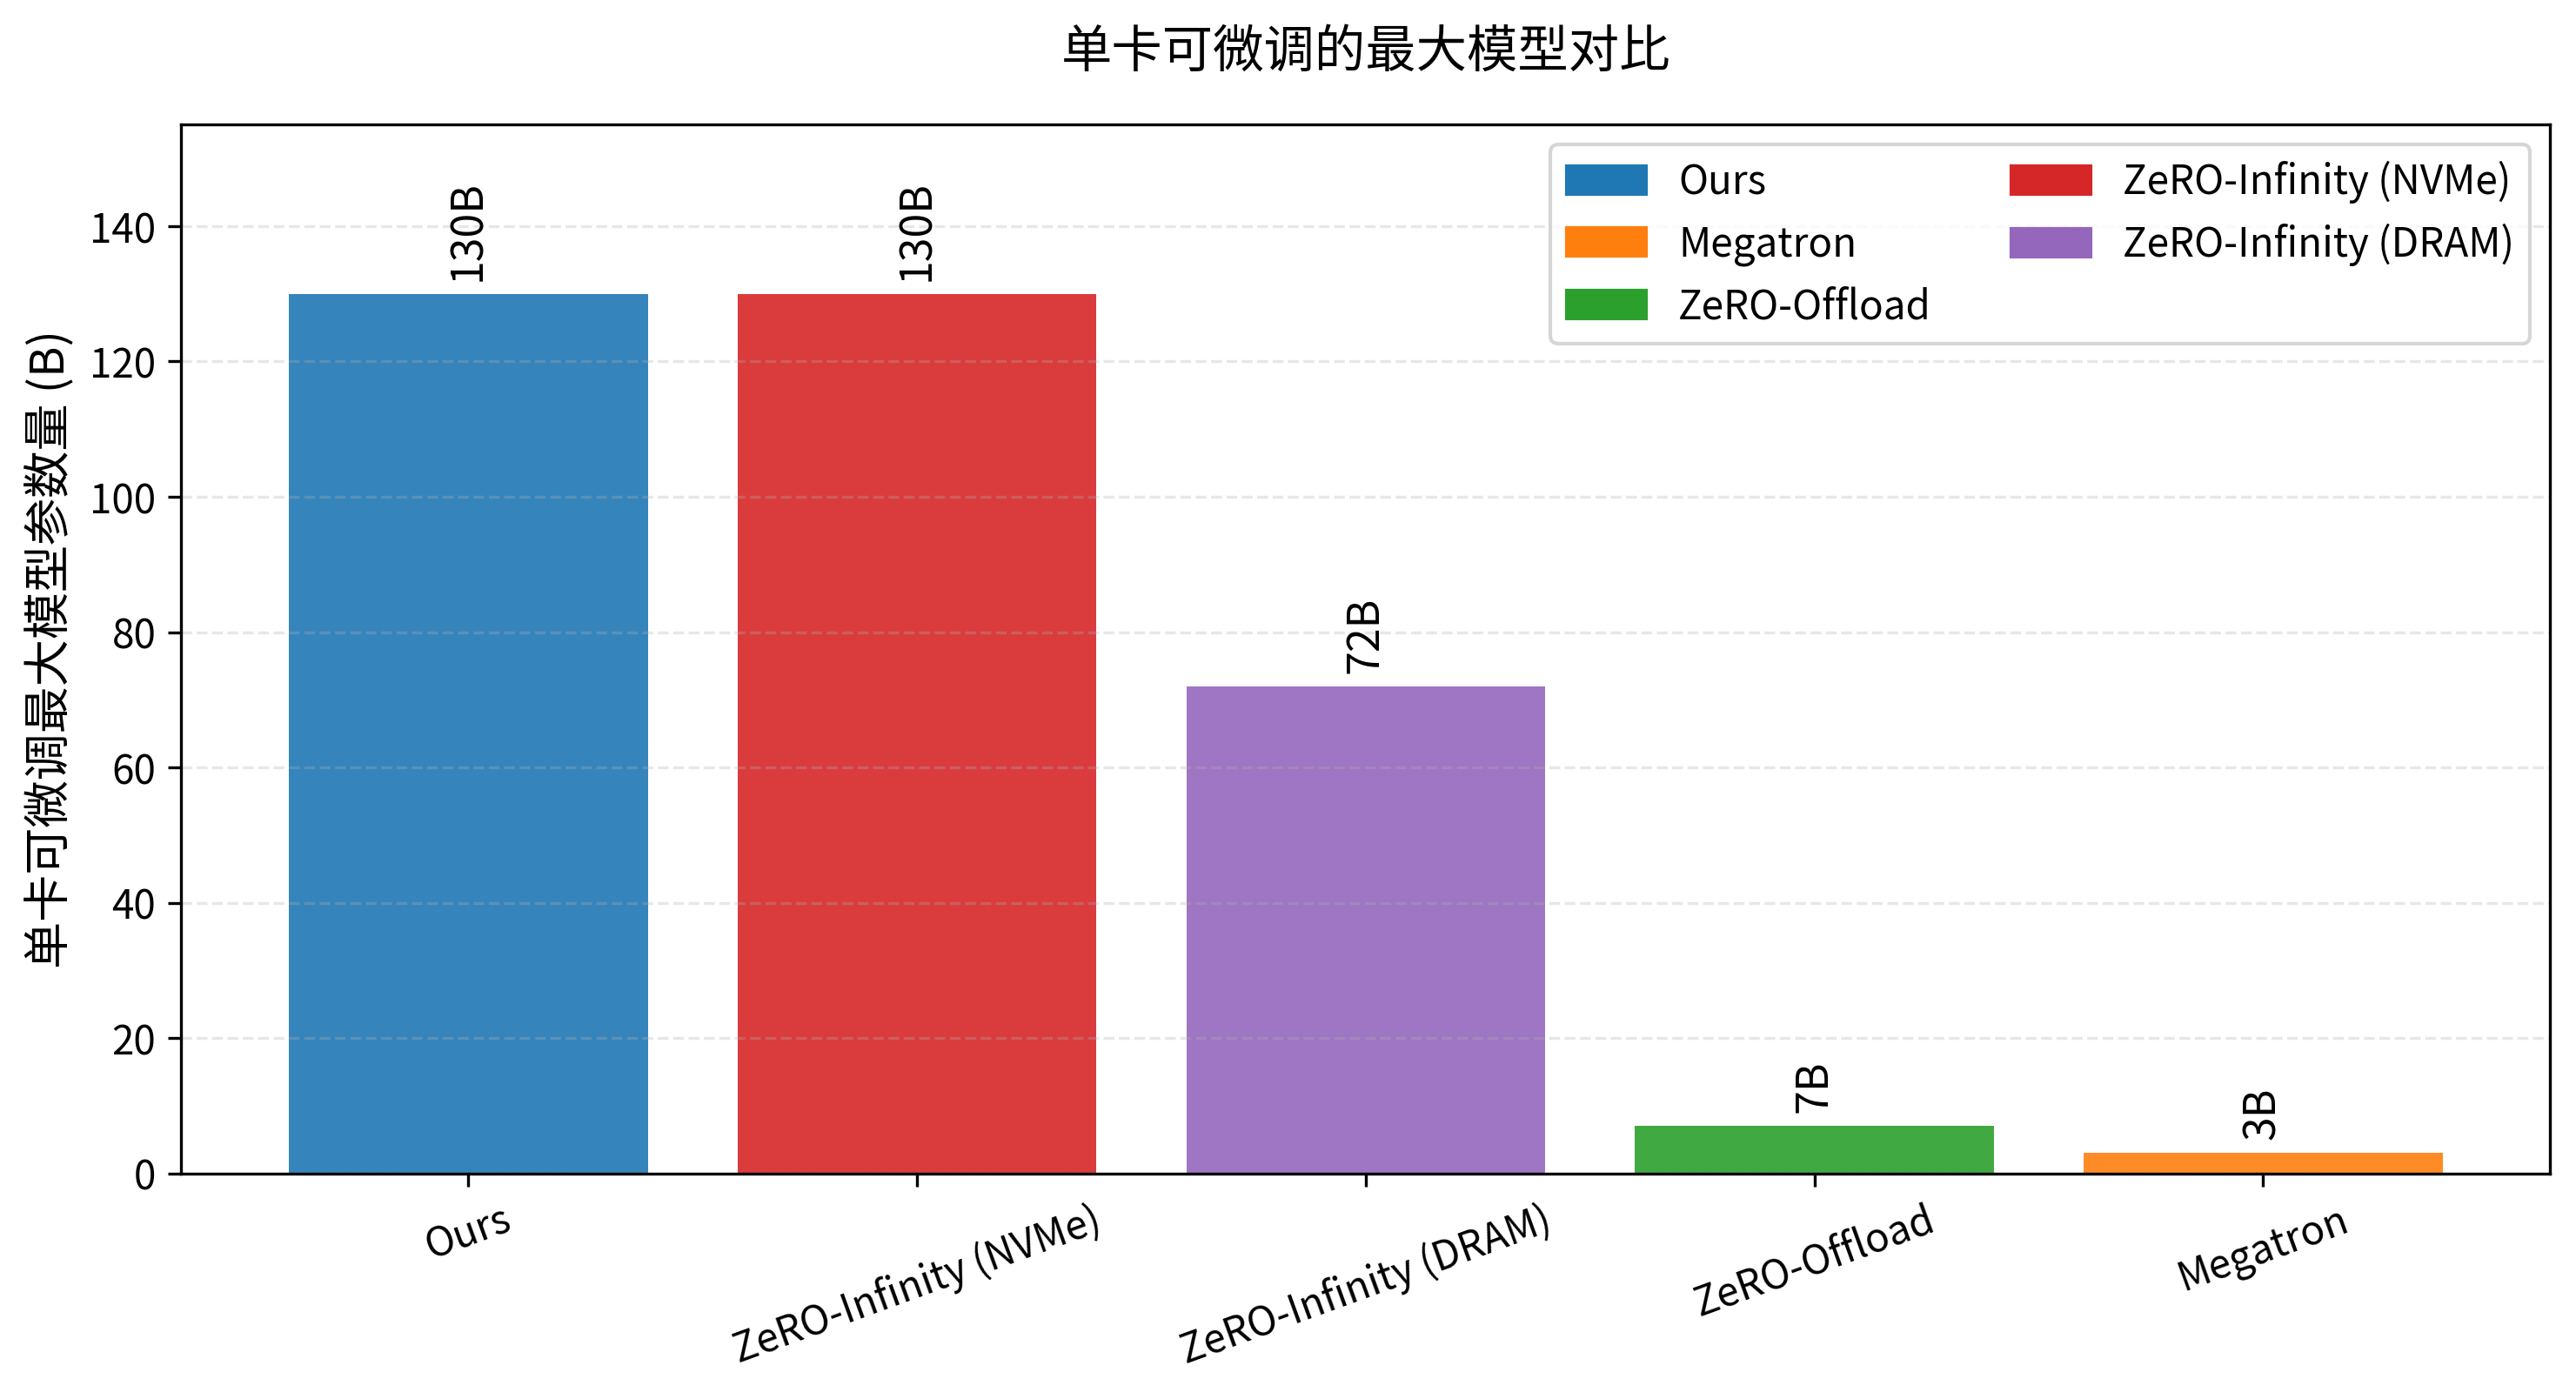
\includegraphics[width=1\textwidth]{figure/max_tranable_single.png}
  \caption{实验范围内单卡最大微调参数量对比}
  \label{fig:max-trainable-params}
\end{figure}

本系统在单机 8 卡情形下的微调规模相比 Megatron-Mindspeed 和
 ZeRO-Infinity-DRAM
亦更优。单机情形本系统可微调 250B 模型，而后者依然受限于内存大小，无法
微调 130B 及以上模型。而 ZeRO-Infinity-NVMe 在理论上通过 NVMe 扩展可支持更大规模模型参数，
但其性能受限于 NVMe 带宽，
导致参数交换开销远大于计算开销，从而难以实现有效微调。

本系统在同一参数量级下还能实现更大的微批次下的微调，
这是因为本系统实现了激活值的卸载，相比其他系统中
HBM 需要容纳所有隐藏层，本系统 HBM 只需要
容纳活跃层的 3 层激活值。
这一设计有利于通过增大微批次来提高单元计算的强度，以此提升系统吞吐。

\begin{figure}[!htbp]
  \centering
  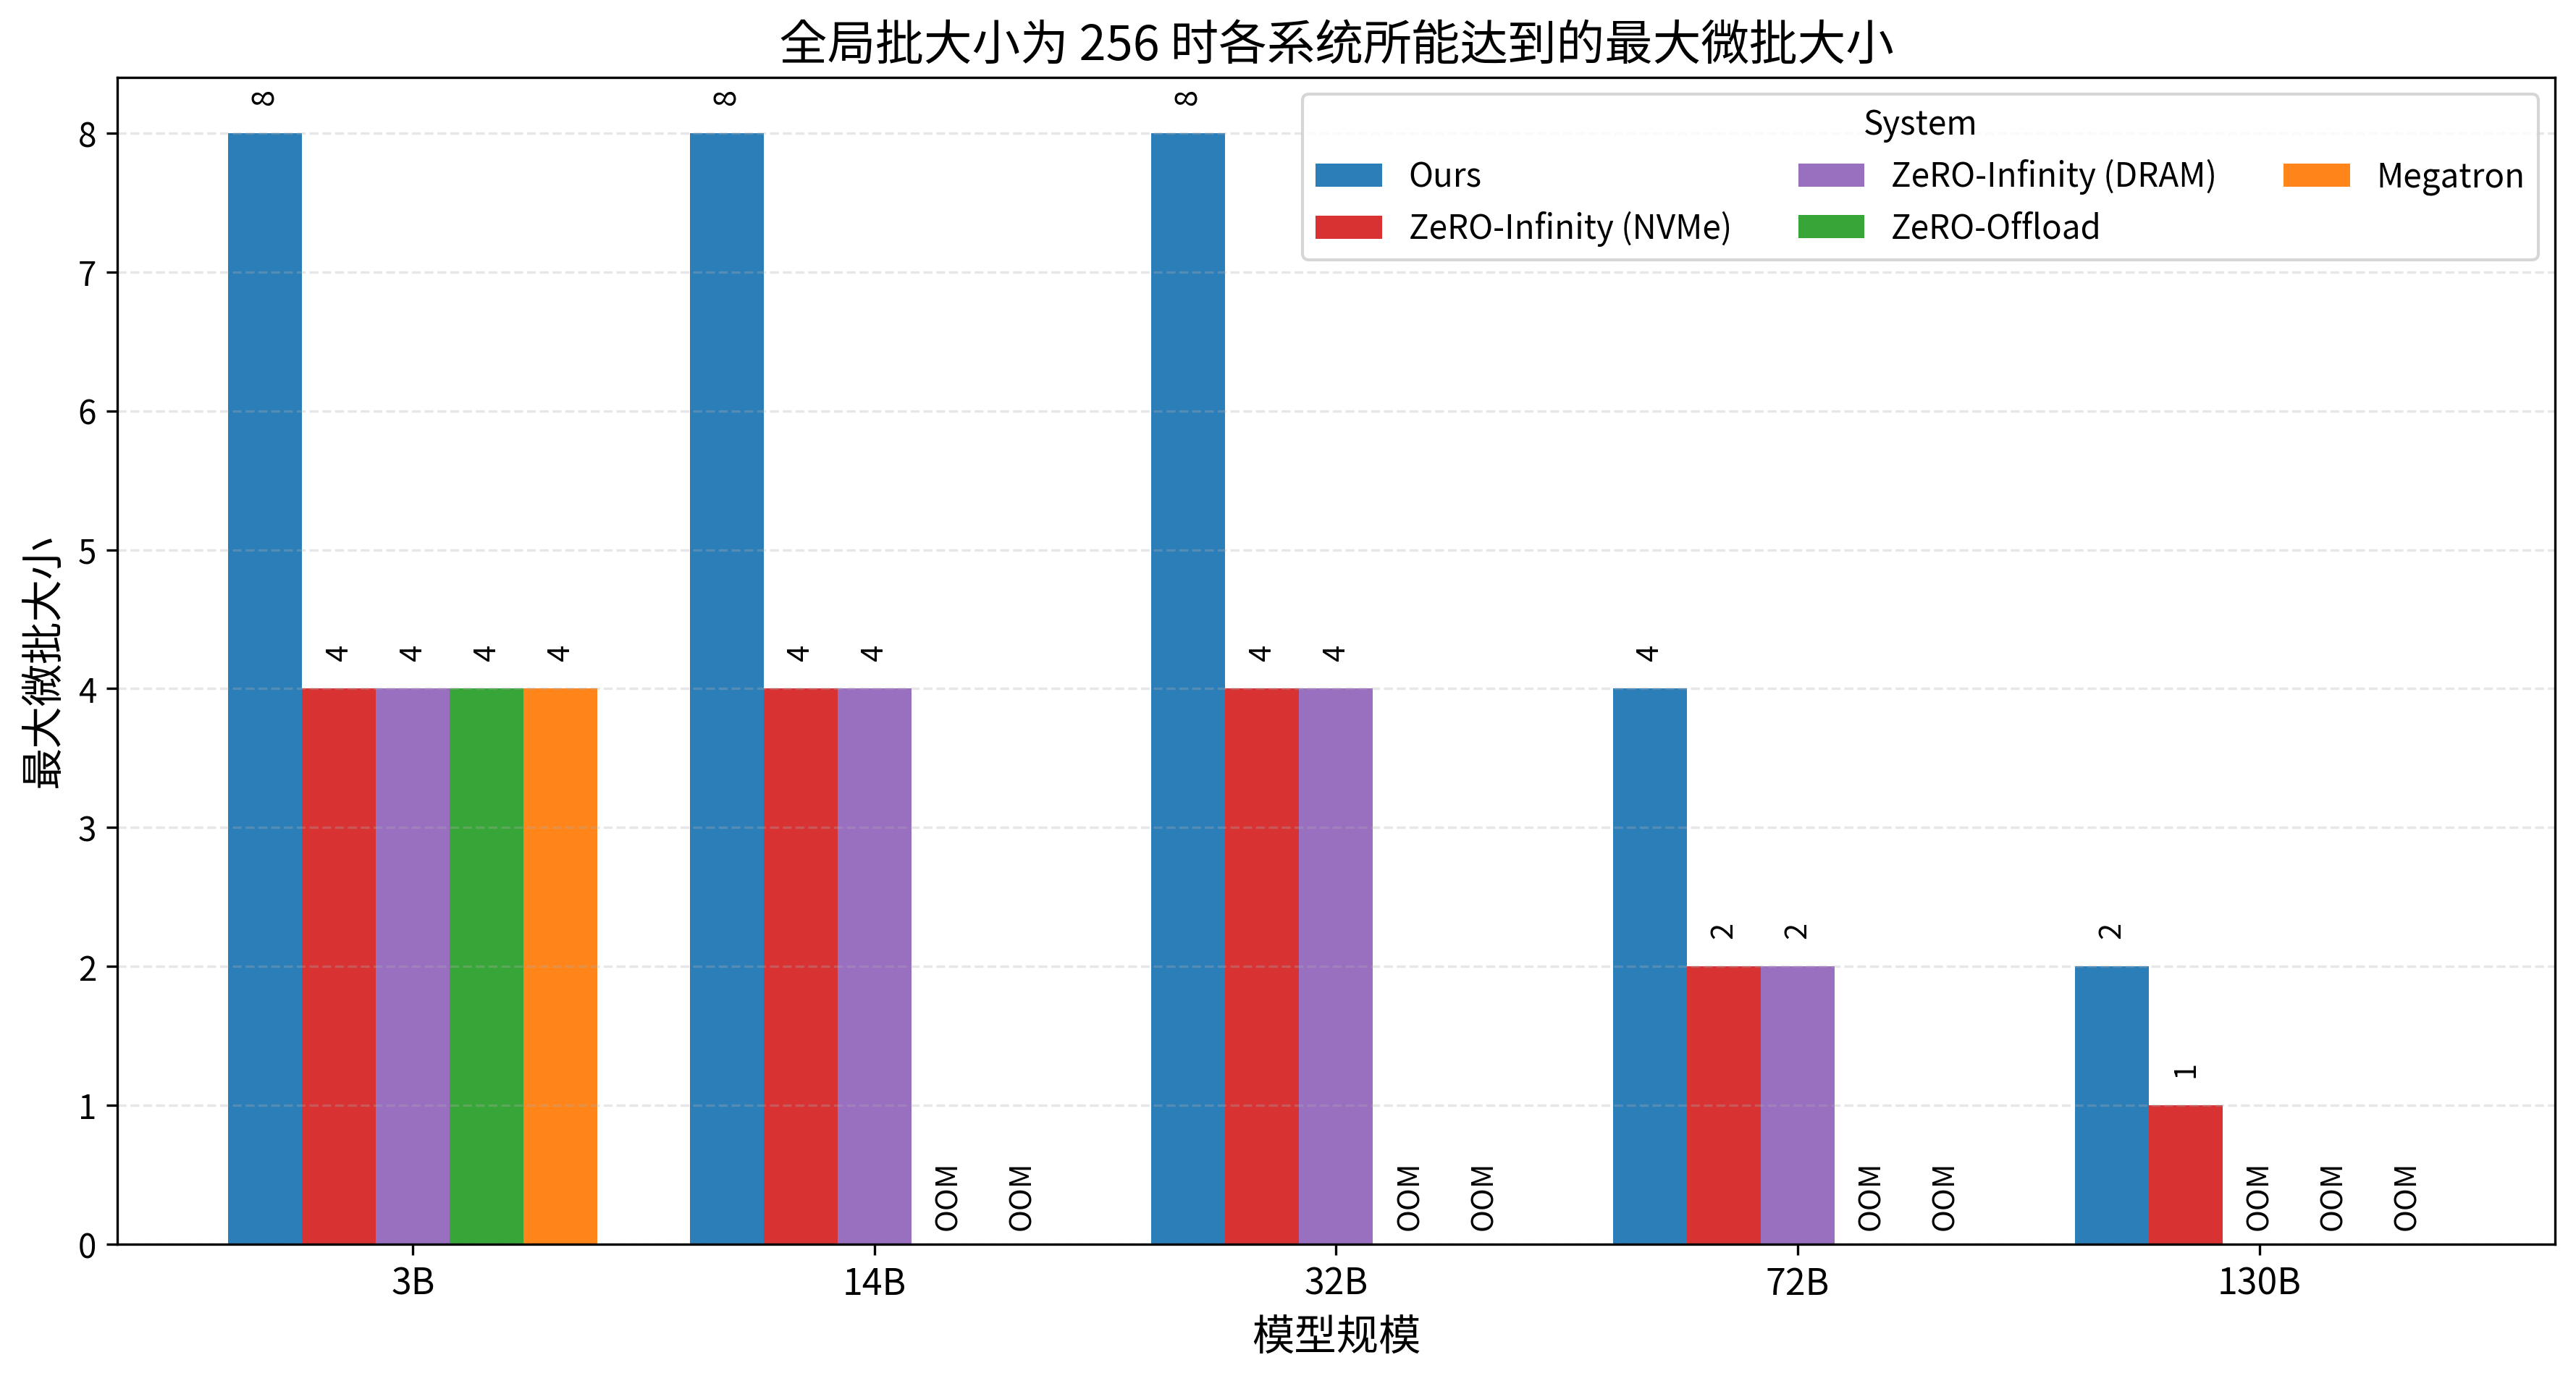
\includegraphics[width=1\textwidth]{figure/max_trainable_bs_single.png}
  \caption{实验范围内单卡最大微调微批次大小对比}
  \label{fig:max-trainable-mbs}
\end{figure}


\section{性能}
该系统在微调过程中相对于 Megatron-Mindspeed 吞吐有所下降，
而相比于 Zero 系列系统更优。
例如在单卡情形下固定序列长度为 4096，全局批次大小为 256，
局部批次分别取可以不发生 OOM 异常的最大值，如前一章所述。
在 Qwen2.5-3B 模型下微调一轮，可以发现在 3B 参数量下，本系统的吞吐低于
Megatron-Mindspeed 10\% 以内。
主要原因在于相比原生系统，虽然理论上计算可掩盖数据传输，但系统在运行时引入
了 Hook 和槽位管理的同步开销，另外一些小模块
如输出处的 Norm 模块比 Transformer 模块偏小，IO 时间不能掩盖。

在单卡情形下，14B 以上的模型在 Megatron-Mindspeed 框架下
和 ZeRO-Offload 框架下无论微批设置为多少均会发生 OOM，这是由于在 14B 以上的模型配置下，
单卡 HBM 无法容纳整个模型的参数、梯度和激活值。而 ZeRO-Infinity 框架和本框架
可以运行微调任务，本框架吞吐高于 ZeRO-Infinity，这主要源于系统设计更好
掩盖了数据传输，同时综合运用 CPU 侧算力。对于 130B 模型，ZeRO-Infinity 只
将主机 DRAM 作为卸载目标时会发生主机侧 OOM，而卸载到 NVMe 侧的 ZeRO-Infinity
框架则受限于 IO 带宽，在吞吐指标上显著小于本系统。

\begin{figure}[!htbp]
  \centering
  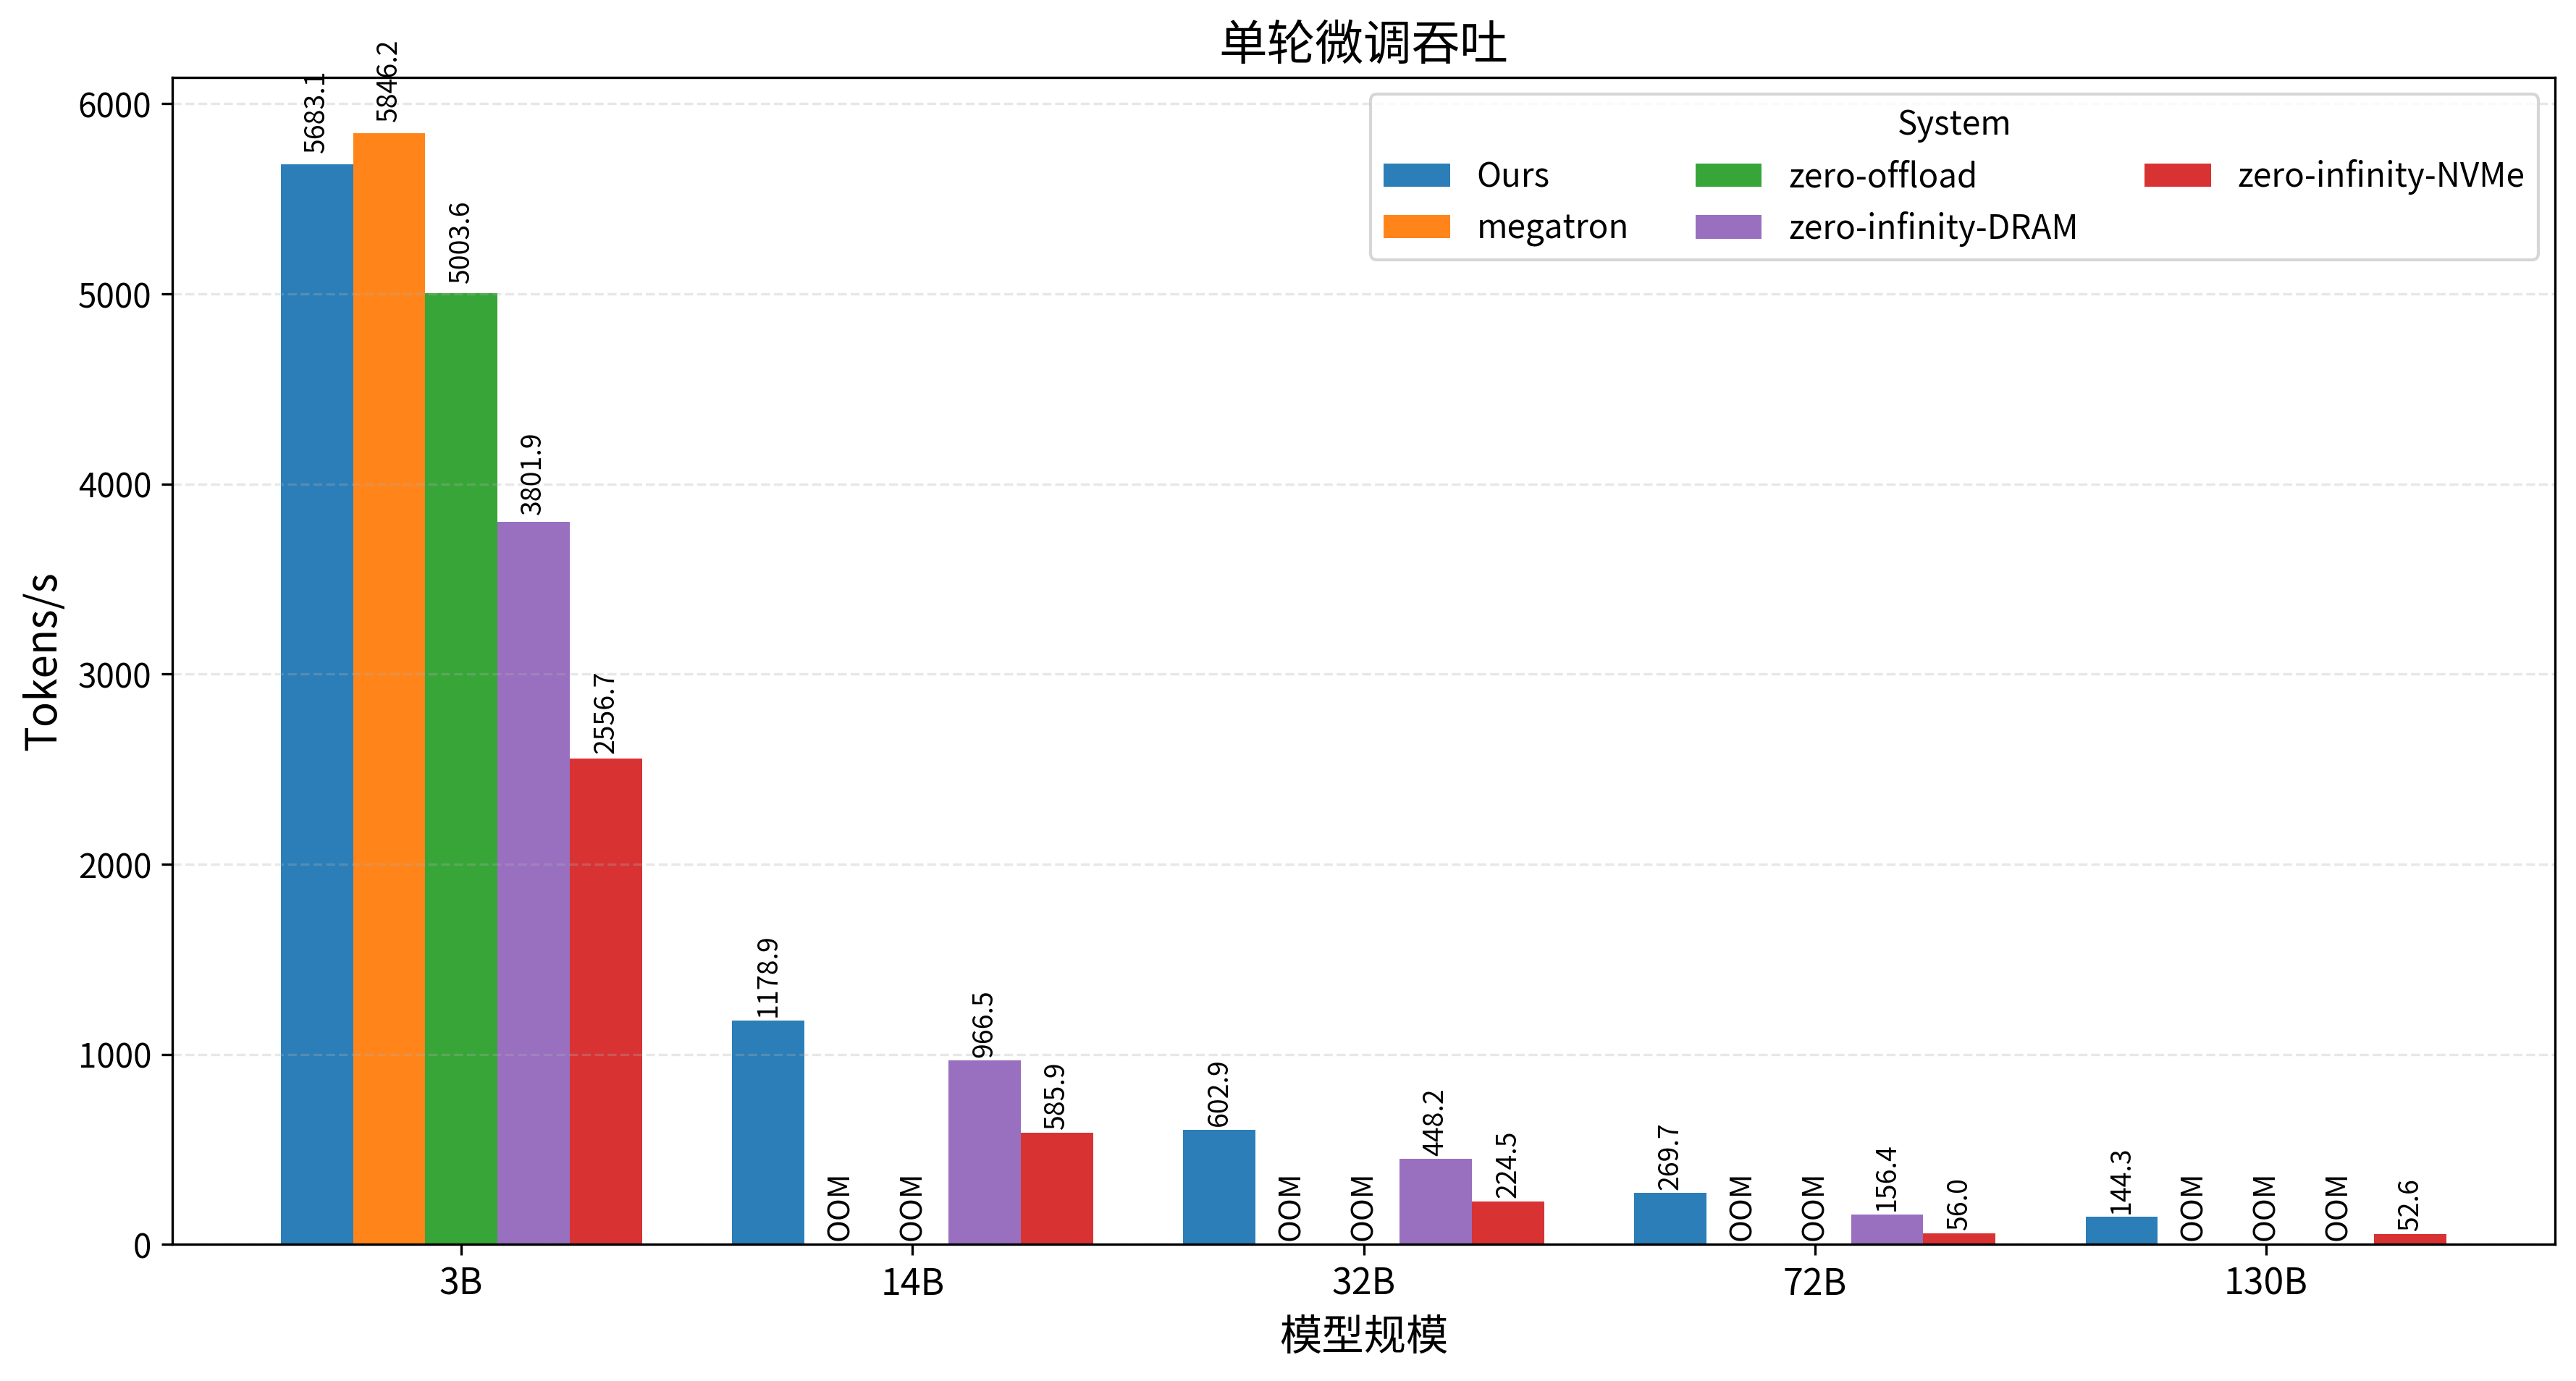
\includegraphics[width=1\textwidth]{figure/single_throughput.png}
  \caption{单卡微调不同系统和参数量吞吐量对比}
  \label{fig:single-throughput}
\end{figure}

在单节点情形下，Megatron-Mindspeed 系统依然不能
微调 72B 及更大模型，而 ZeRO 系列框架在绝大部分配置下性能
比本系统吞吐量低。
对 72B 模型，本系统单卡吞吐为 ZeRO-Infinity-NVMe 的 4.8 倍；
随卡数增加 NVMe 带宽被多卡分摊、计算侧占比下降，
8 卡时 ZeRO-Infinity-NVMe 与本系统差距缩小但仍落后本系统 17\%。
ZeRO-Infinity-DRAM 在 72B 上所有配置均可运行，8 卡时略优于本系统，
但该优势建立在其单机 DRAM 能容纳 72B 参数+优化器状态的前提下，不具备向更大模型扩展的能力。

\begin{figure}[!htbp]
  \centering
  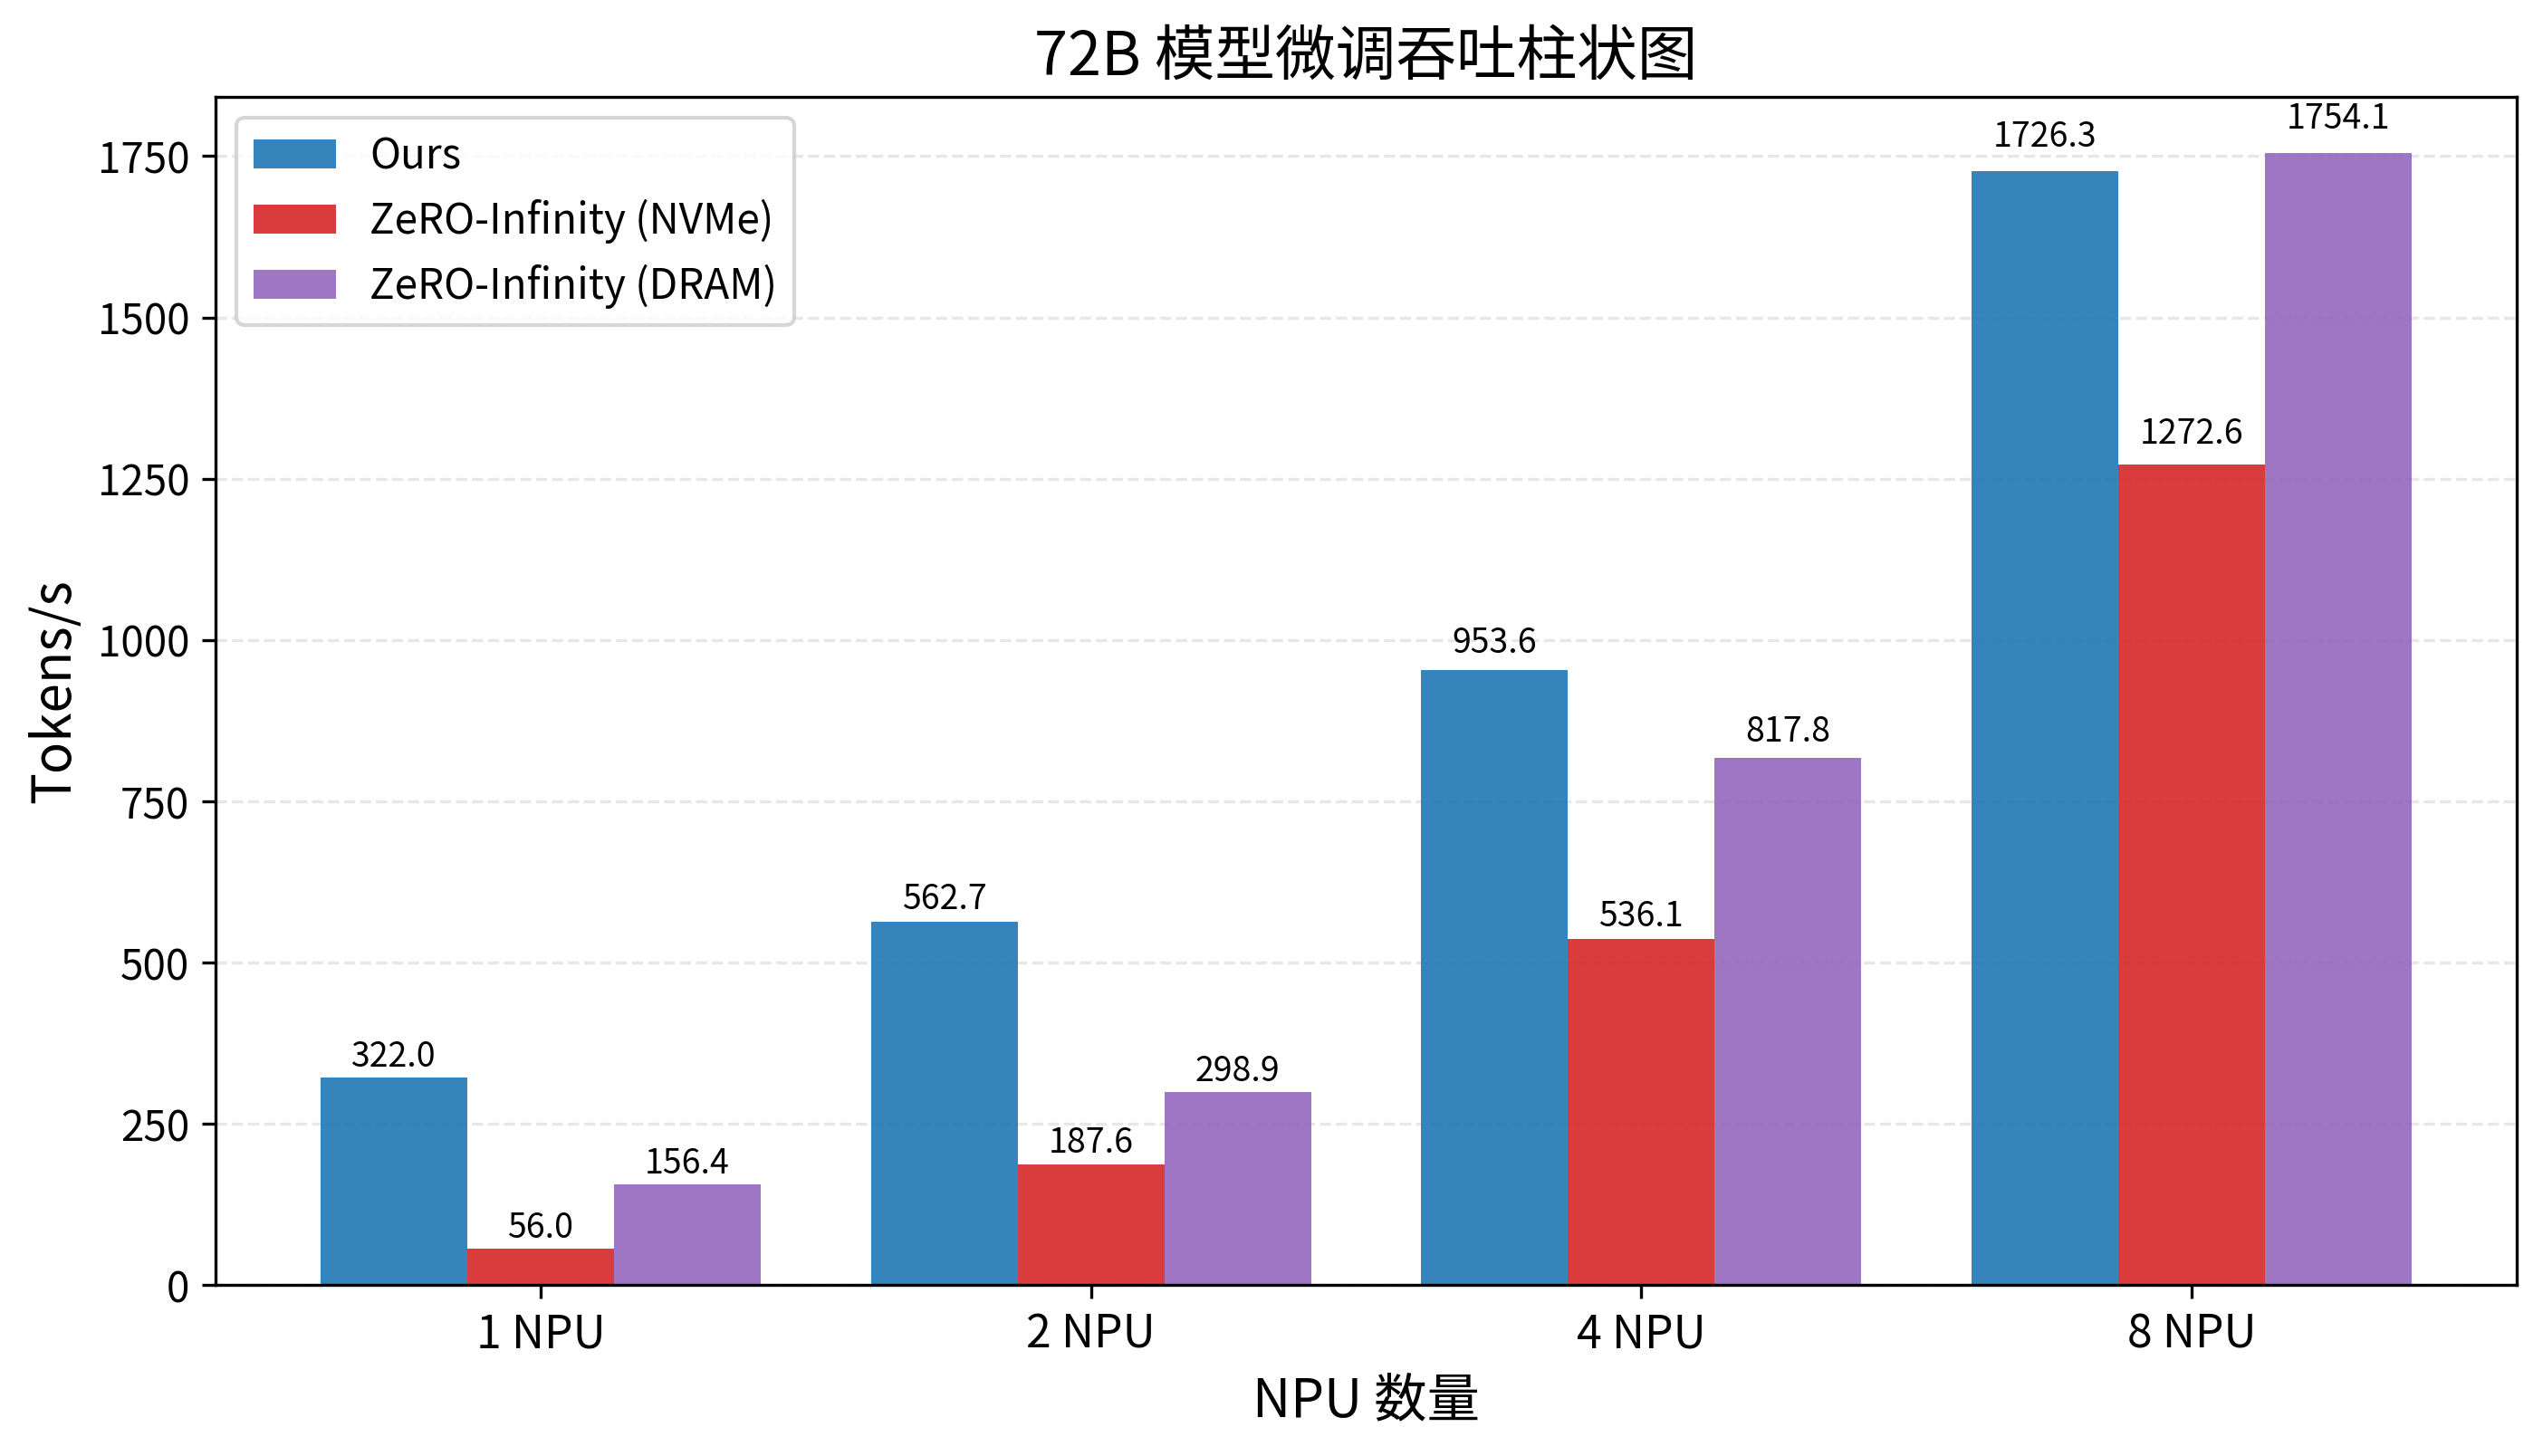
\includegraphics[width=1\textwidth]{figure/72B_node_throughput.png}
  \caption{不同系统微调单节点 72B 模型吞吐量对比}
  \label{fig:node72-throughput}
\end{figure}

对 130B 模型，ZeRO-Infinity-DRAM 在所有卡数配置下均发生主机侧 OOM，无法完成微调，
有 ZeRO-Infinity-NVMe 与本系统可比较。
本系统单卡即可完成 130B 微调，吞吐 144~tokens/s；
2/4/8 卡分别达到 262、499、825~tokens/s。
ZeRO-Infinity-NVMe 在 1/2 卡下几乎完全受 NVMe 带宽限制，
吞吐停滞在 53~tokens/s 附近，本系统相对其加速比达 2.7$\sim$4.8 倍；
4/8 卡虽因多路 NVMe 并行吞吐上升至 180、484~tokens/s，
仍显著低于本系统对应配置，差距在 1.7$\sim$2.8 倍之间。
这一结果与第三章的重叠条件分析一致：
NVMe 带宽难以支撑前后向阶段逐层高频参数访问，
而将参数和主梯度限制在 DRAM 路径、
仅将优化器状态下沉到 NVMe，
可以同时获得容量扩展和较高吞吐。

\begin{figure}[!htbp]
  \centering
  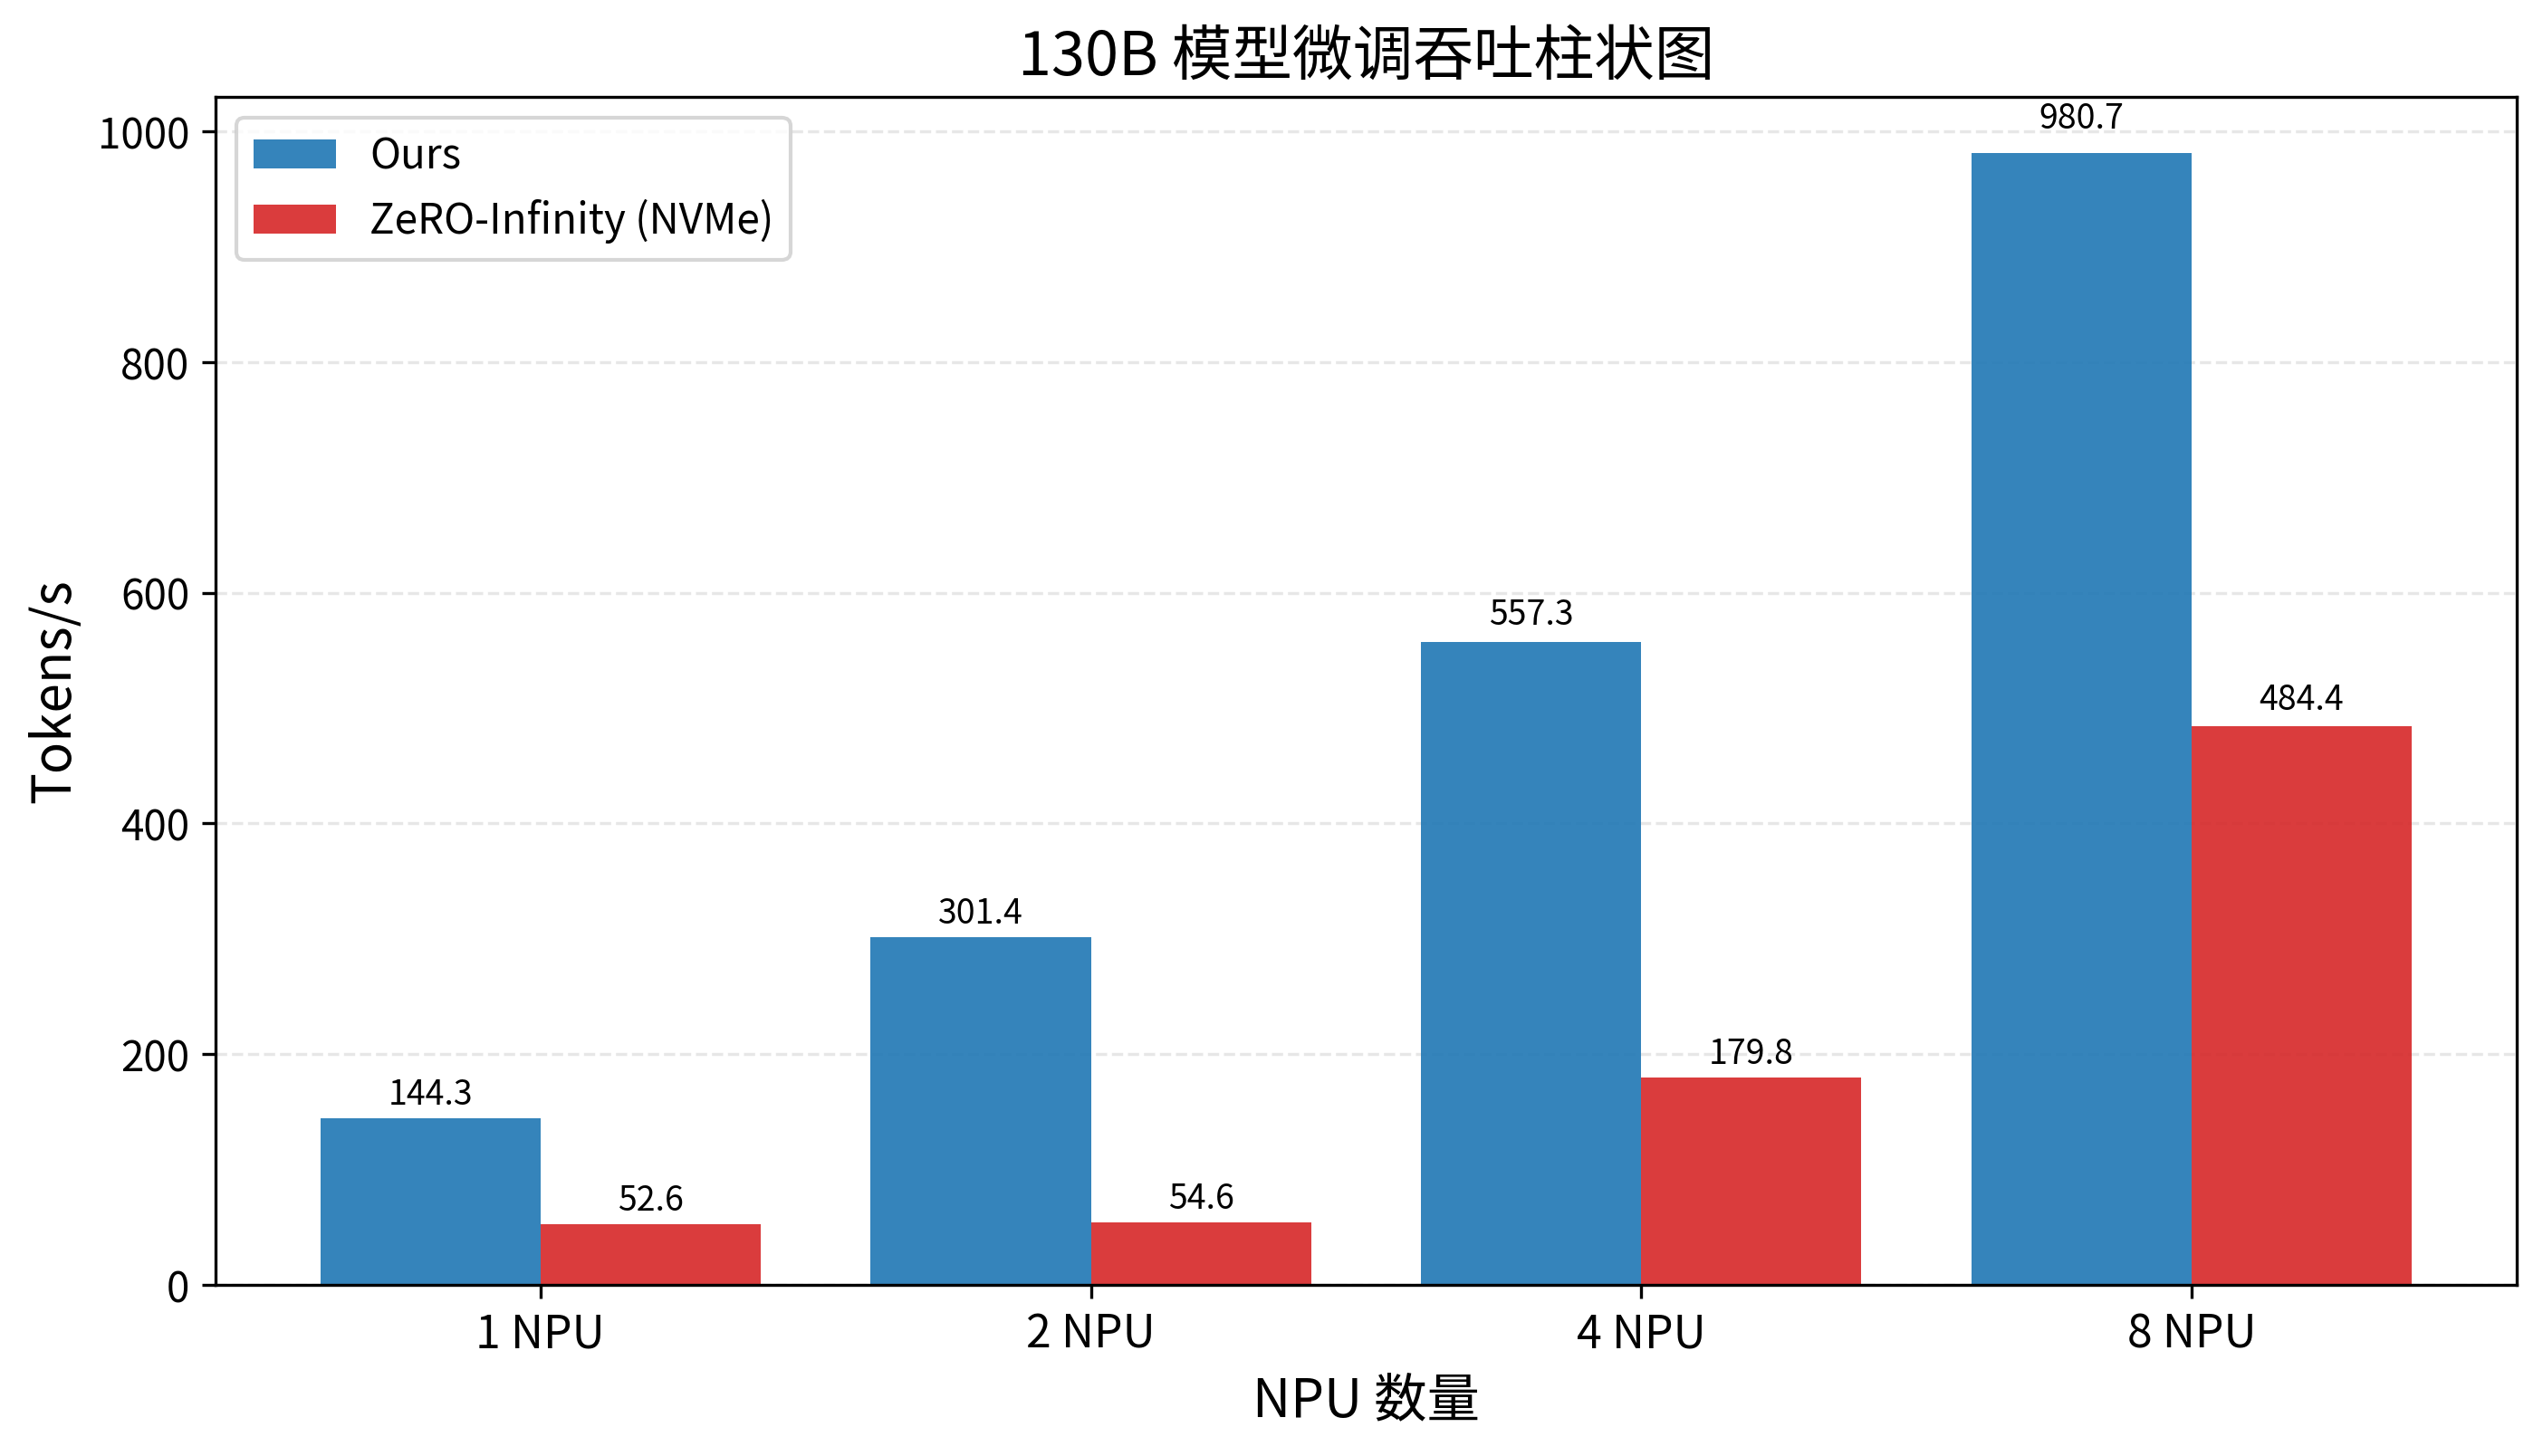
\includegraphics[width=1\textwidth]{figure/130B_node_throughput.png}
  \caption{不同系统微调单节点 130B 模型吞吐量对比}
  \label{fig:node130-throughput}
\end{figure}

\section{消融实验}
TODO 提纲挈领

\subsection{预取引擎的实验}


\subsection{优化器}
本系统的优化器子模块完全在 CPU 上执行，同时状态常驻于 NVMe SSD，
为了防止其 CPU 计算和 IO 时长成为瓶颈，系统进行了算子和 IO 计算重叠
的优化。
为验证其效果，在单卡的统一配置下，
测量不同参数量模型单轮迭代中的优化器耗时，结果如图~\ref{fig:opt-time}所示。

\begin{figure}[!htbp]
  \centering
  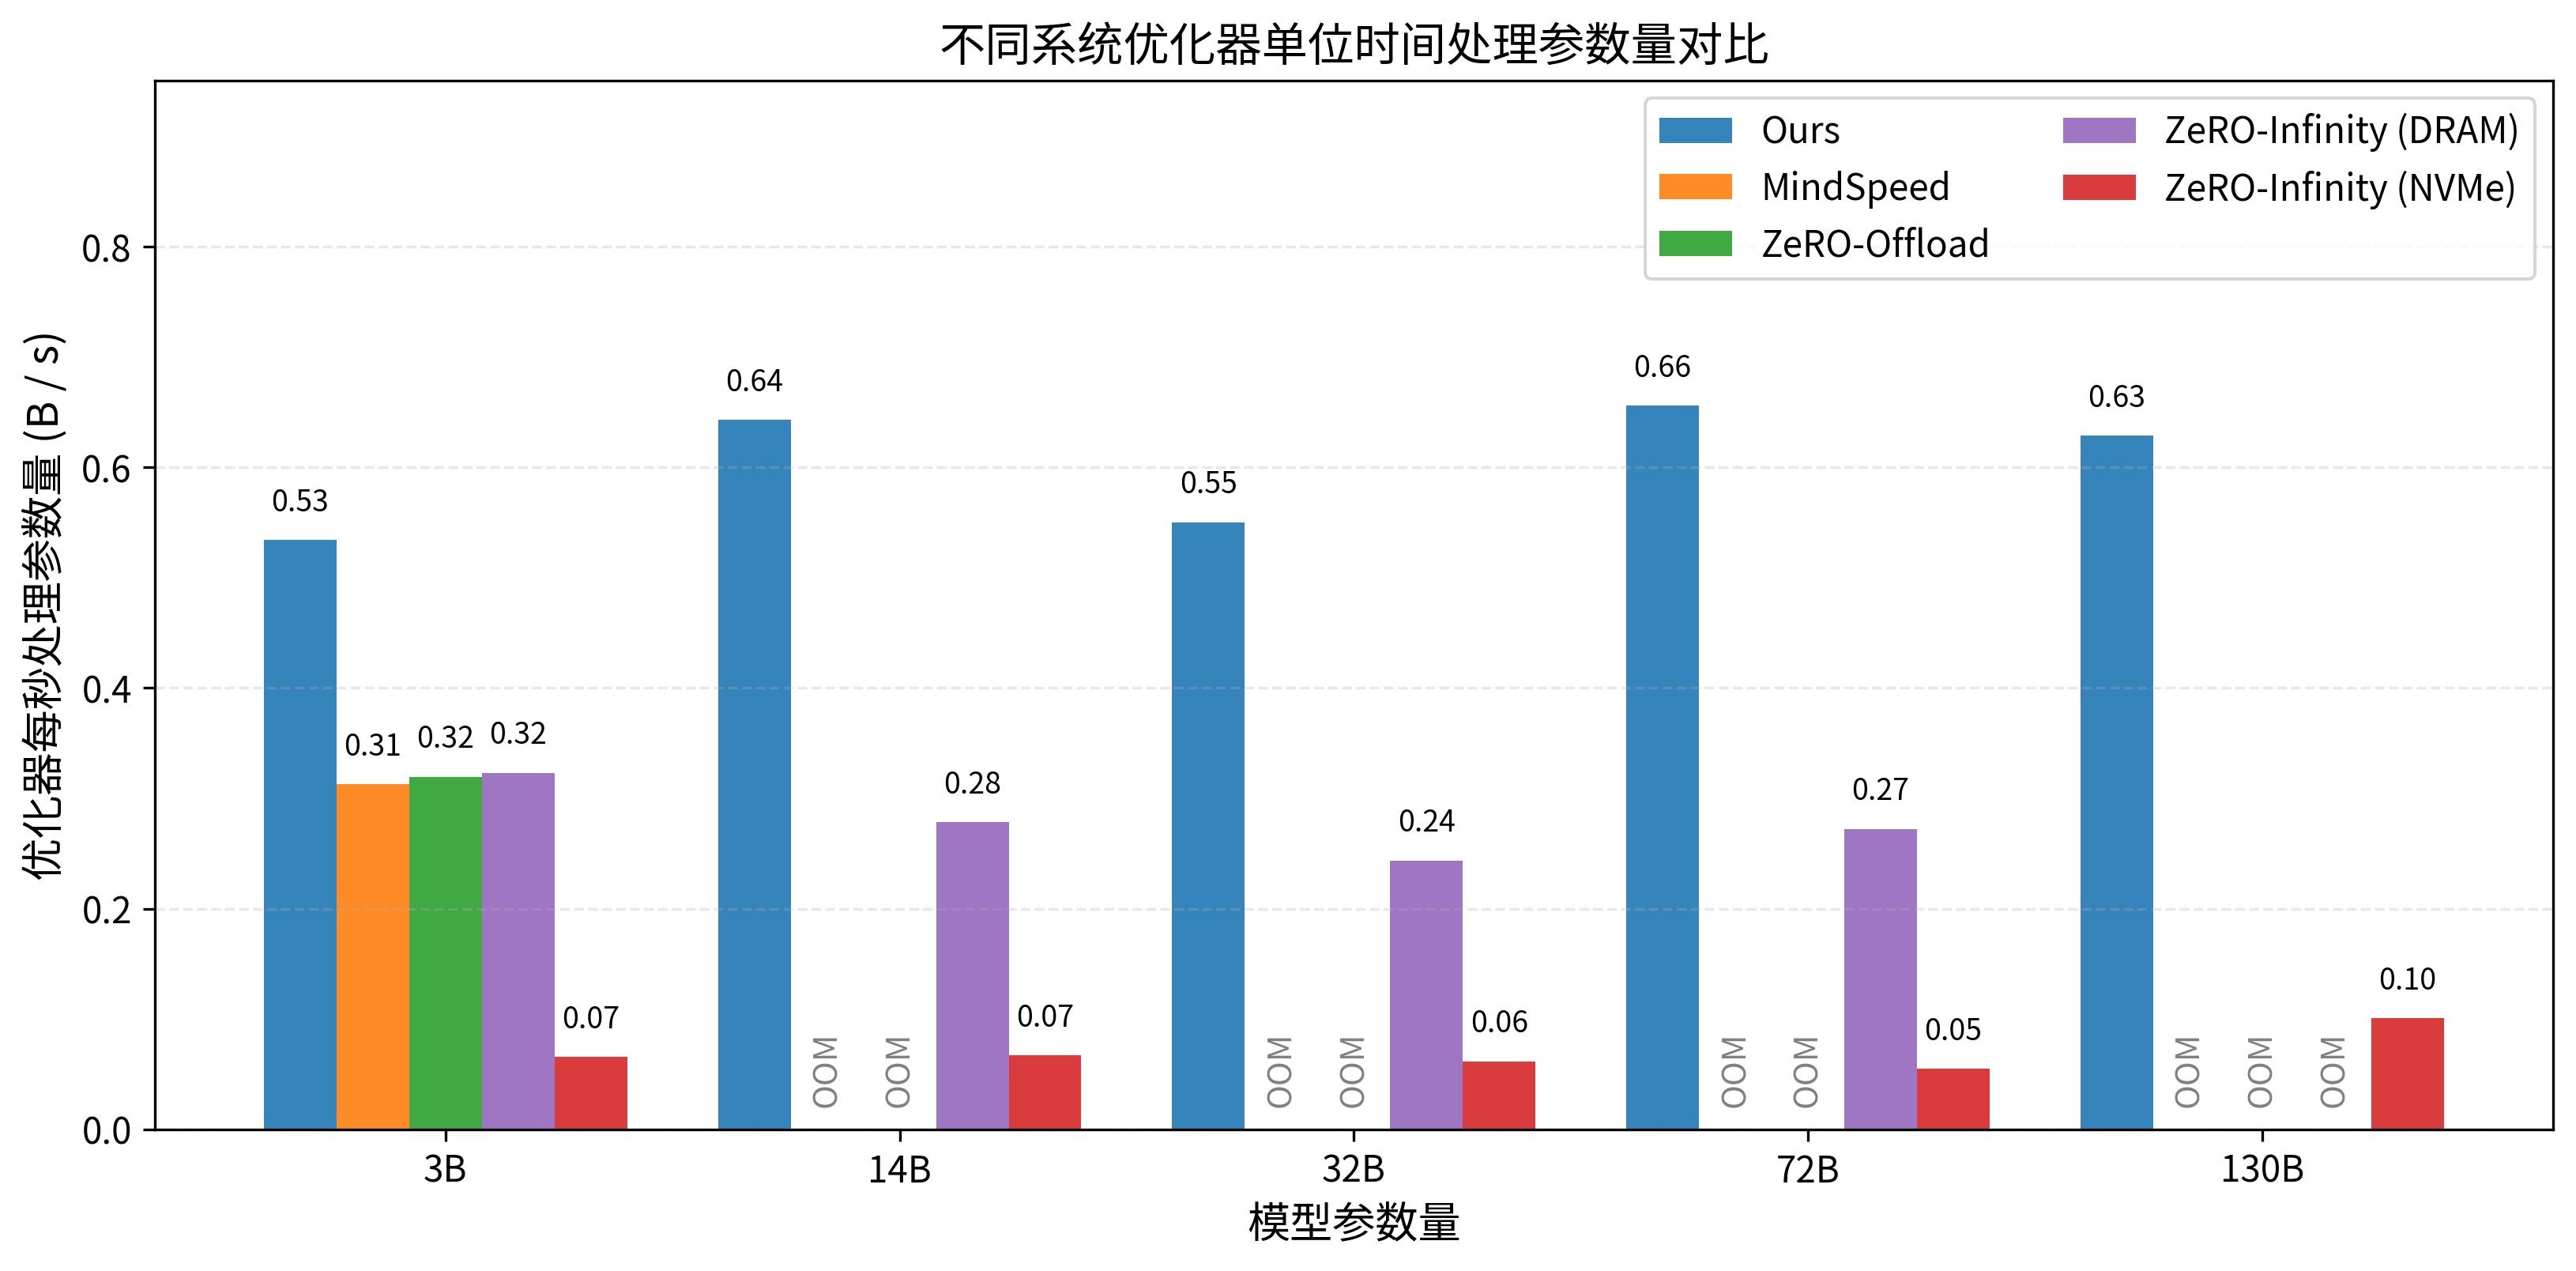
\includegraphics[width=1\textwidth]{figure/optim_throughput.png}
  \caption{不同系统单轮优化器吞吐量}
  \label{fig:opt-time}
\end{figure}

从耗时看，本系统的优化器在单卡情况下所有参数量级下均为最快。
3B 时相对 Megatron、ZeRO-Offload、ZeRO-Infinity-DRAM 领先约 40\%，
14B$\sim$72B 相对 ZeRO-Infinity-DRAM 保持 2.2$\sim$2.5$\times$ 领先，
相对 ZeRO-Infinity-NVMe 领先 8$\sim$11$\times$；
130B 下仅 ZeRO-Infinity-NVMe 可运行，本系统相对其仍领先 6.2$\times$。

在单卡，批大小为 256 时，本系统的优化器耗时占单轮迭代的比例
稳定在 2.4\%$\sim$3.2\% 区间，
卸载代价压到可忽略。

% !Mode:: "TeX:UTF-8"
\cleardoublepage
\phantomsection
\addcontentsline{toc}{chapter}{参考文献}
\bibliography{data/bibs}
\cleardoublepage

\end{document}

